\documentclass[a4paper, 11pt]{article}
\usepackage{graphicx} % Required for inserting images
\usepackage{subcaption}
% pseudocode 
\usepackage{algorithm}
\usepackage{algpseudocode}
\usepackage{underscore}

\usepackage{enumitem}

\usepackage{hyperref}

\usepackage{svg}

\usepackage{amssymb, amsfonts, amsmath, amsthm}

\usepackage[most]{tcolorbox}
\tcbuselibrary{theorems}

\usepackage{cleveref}
\makeatletter
\newcommand\xlongrightarrow[2][]{%
  \ext@arrow 9999{\longleftrightarrowfill@}{#1}{#2}}
\newcommand\longrightarrowfill@{%
  \arrowfill@\leftarrow\relbar\rightarrow}
\makeatother

\newtcbtheorem[use counter=equation]{theorem}{Theorem}%
{colback=white,colframe=black,fonttitle=\bfseries}{th}

\newtcbtheorem[use counter=equation]{corollary}{Corollary}%
{colback=white,colframe=black,fonttitle=\bfseries}{cor}

\newtcbtheorem[use counter=equation]{lemma}{Lemma}%
{colback=white,colframe=black,fonttitle=\bfseries}{lem}

\newtcbtheorem[use counter=equation]{proposition}{Proposition}%
{colback=white,colframe=black,fonttitle=\bfseries}{prop}

\newtcbtheorem[use counter=equation]{definition}{Definition}%
{colback=white,colframe=black,fonttitle=\bfseries}{def}

% \newtcbtheorem[use counter=equation]{remark}{Remark}%
% {colback=white,colframe=black,fonttitle=\bfseries}{rem}

\theoremstyle{remark} 
\newtheorem{remark}[equation]{Remark} 

\newtcbtheorem[use counter=equation]{ex}{Example}%
{colback=white,colframe=black,fonttitle=\bfseries}{ex}

\newtcbtheorem[use counter=equation]{notation}{Notation}%
{colback=white,colframe=black,fonttitle=\bfseries}{not}

\newtcbtheorem[use counter=equation]{terminology}{Terminology}%
{colback=white,colframe=black,fonttitle=\bfseries}{term}

\title{Reduced-Order Overlapping Schwarz Waveform Relaxation Method}
\author{Anar Abdullayev\\[2ex]\textit{Faculty of Mathematics and Computer Science, University of Münster}}
\date{\today}

\usepackage{geometry}
\geometry{
a4paper, 
left = 1.5cm,
right = 1.5cm,
top = 2.54cm,
bottom = 2.54cm
}

\begin{document}

\maketitle

\section{Schwarz Formulations}

\subsection{Model Problem}
We consider the following initial-boundary value problem for the heat equation
\begin{align*}
    \dfrac{\partial u}{\partial t} &= \Delta u + f(x, t), \qquad x\in \Omega, \,\,\,\,\quad 0<t<T,\\
    u(x, t) &= g(x, t), \hspace{52pt} x\in \partial\Omega, \quad 0<t<T,\\
    u(x, 0) &= u_{0}(x), \hspace{55pt} x\in \Omega,
\end{align*}
where $\Omega\subset \mathbb{R}^{d}$ is a bounded Lipschitz domain. Suitable regularity and compatibility assumptions on the data $f$, $g$, and $u_{0}$ will be specified where required.

\newpage
\subsection{Domain Decompositions}
In this subsection, we present definitions of non-overlapping and overlapping domain decompositions. For overlapping decompositions, we introduce several variants, including minimal overlapping, uniform overlapping, and nonuniform overlapping, which differ in how the subdomains extend beyond their base regions. These definitions are provided for both geometric (non-mesh-aligned) and mesh-conforming decompositions. We also highlight alternative definitions and approaches that may appear in the literature.

\subsubsection{Geometric Decomposition}

This subsection considers the geometric decomposition of a bounded domain $\Omega \subset \mathbb{R}^{d}$, where $\Omega$ is a non-empty, connected, open, and bounded subset of $\mathbb{R}^{d}$. While $\Omega$ may have a smooth or curved boundary $\partial\Omega$, we assume that $\partial\Omega$ satisfies the strong local Lipschitz condition so that standard Sobolev space and trace results remain valid (see, e.g., Adams and Fournier~\cite{AdamsFournier2003}). We first introduce a non-overlapping decomposition of such a domain and then proceed to the overlapping decomposition.

\begin{definition}{Non-overlapping Domain Decomposition}{nonoverlapdecomp}
Let $\Omega \subset \mathbb{R}^d$ be a bounded domain. A \textbf{non-overlapping decomposition} of $\Omega$ is a finite collection of subdomains $\{\Omega_{i}\}$ such that
\begin{equation*}
    \Omega_{i} \cap \Omega_{j} = \emptyset \quad\text{ for } i \neq j,
\end{equation*}
and
\begin{equation*}
    \overline{\Omega} = \bigcup\overline{\Omega}_{i}.
\end{equation*}
For each subdomain $\Omega_i$, let
\begin{equation*}
    \Gamma_{i} := \partial \Omega_i
\end{equation*}
denote its boundary. The boundary can be decomposed into two disjoint parts, 
\begin{equation*}
    \Gamma_{i} = \Gamma_{i}^{\text{ext}} \cup \Gamma_{i}^{\text{int}},
\end{equation*}
where
\begin{equation*}
    \Gamma_{i}^{\text{ext}} := \partial \Omega_i \cap \partial \Omega
\end{equation*}
is the \textbf{exterior boundary}, and
\begin{equation*}
    \Gamma_{i}^{\text{int}} := \partial \Omega_{i} \setminus \partial\Omega
\end{equation*}
is the \textbf{interface boundary}, which is shared with neighboring subdomains.
\end{definition}
\noindent After introducing a non-overlapping decomposition, it is useful to classify subdomains according to whether they touch the boundary of the global domain. This distinction is important in domain decomposition methods, as boundary subdomains are adjacent to the global boundary $\partial \Omega$, whereas interior subdomains are entirely surrounded by other subdomains. Formally, we define boundary and interior subdomains as follows.
\begin{definition}{Boundary and Interior Subdomains}{subdomain_type}
Let $\{\Omega_i\}_{i=1}^N$ be a non-overlapping decomposition of a bounded domain $\Omega \subset \mathbb{R}^d$. A subdomain $\Omega_i$ is called a \textbf{boundary subdomain} if its exterior boundary is non-empty,
\begin{equation*}
    \Gamma_i^{\text{ext}} \neq \emptyset,
\end{equation*}
and it is called an \textbf{interior subdomain} if its exterior boundary is empty,
\begin{equation*}
    \Gamma_i^{\text{ext}} = \emptyset.
\end{equation*}
\end{definition}
\noindent Each subdomain $\Omega_i$ has a boundary $\Gamma_i = \partial \Omega_i$, which can be split into the exterior boundary $\Gamma_i^{\text{ext}}$ and the interface (interior) boundary $\Gamma_i^{\text{int}}$.  
The exterior boundary indicates whether the subdomain touches the boundary of the global domain $\Omega$, while the interface boundary corresponds to the portion of $\partial \Omega_i$ shared with neighboring subdomains. The union of all interface boundaries across the decomposition forms the \textbf{interface} (or \textbf{skeleton}) of the domain decomposition (see Brenner and Scott~\cite{BrennerScott2008}). This interface is central in domain decomposition methods, as it represents the region where subdomains interact and exchange information.
\begin{definition}{Interface (Skeleton)}{interface_skeleton}
Let $\{\Omega_i\}_{i=1}^N$ be a non-overlapping decomposition of $\Omega$. The \textbf{interface} (also called the \textbf{skeleton}) of the decomposition is defined as
\begin{equation*}
    \Gamma^{\text{int}} := \bigcup\Gamma_{i}^{\text{int}}.
\end{equation*}
\end{definition}
\noindent While non-overlapping decompositions partition the domain into disjoint subdomains, it is often advantageous in numerical methods to consider subdomains that may partially overlap. Overlapping subdomains allow regions to be shared between neighboring subdomains, facilitating the transfer of information across interfaces and improving the convergence and stability of iterative algorithms. To make this concept precise, we provide the following formal definition of an overlapping decomposition.

\begin{definition}{Overlapping Domain Decomposition}{overlapping_decomposition}
Let $\Omega \subset \mathbb{R}^d$ be a bounded domain. An \textbf{overlapping decomposition} of $\Omega$ is a finite collection of subdomains $\{\Omega_{i}\}$ such that
\begin{equation*}
    \Omega = \bigcup\Omega_{i}.
\end{equation*}
For each subdomain $\Omega_i$, let
\begin{equation*}
    \Gamma_{i} := \partial \Omega_i
\end{equation*}
denote its boundary. The boundary can be decomposed into two disjoint parts, 
\begin{equation*}
    \Gamma_{i} = \Gamma_{i}^{\text{ext}} \cup \Gamma_{i}^{\text{int}},
\end{equation*}
where
\begin{equation*}
    \Gamma_{i}^{\text{ext}} := \partial \Omega_i \cap \partial \Omega
\end{equation*}
is the \textbf{exterior boundary}, and
\begin{equation*}
    \Gamma_{i}^{\text{int}} := \partial \Omega_{i} \setminus \partial\Omega
\end{equation*}
is the \textbf{interface boundary}, which is shared with neighboring subdomains.
\end{definition}
\noindent Let us now define what we mean by "neighboring subdomains" and provide an explicit definition.
\begin{definition}{Neighboring Subdomains}{neighboring_subdomains}
Let $\{\Omega_i\}_{i=1}^N$ be a decomposition of a bounded domain $\Omega \subset \mathbb{R}^d$. For $i \neq j$, define 
\begin{equation*}
    \Gamma_{ij} := \Gamma_i^{\text{int}} \cap \overline{\Omega}_j.
\end{equation*}
We say that $\Omega_i$ and $\Omega_j$ are \textbf{neighboring subdomains} if
\begin{equation*}
    \Gamma_{ij} \neq \emptyset.
\end{equation*}
We denote by $\mathcal{N}_i$ the set of indices of all subdomains neighboring $\Omega_{i}$, i.e.,
\begin{equation*}
    \mathcal{N}_i := \{ j \in \{1, \dots, N\} \setminus \{i\} : \Gamma_{ij} \neq \emptyset \}.
\end{equation*}
\end{definition}
This definition holds for both non-overlapping and overlapping decompositions, but it is more relevant in the context of overlapping decompositions, 
where subdomains can share regions. In non-overlapping decompositions, neighboring subdomains typically only touch at their boundaries, while in 
overlapping decompositions, they can have a non-empty intersection. Also, notice that the interface boundary of a subdomain can be expressed as
\begin{equation*}
    \Gamma_{i}^{\text{int}} = \bigcup_{j \in \mathcal{N}_i} \Gamma_{ij},
\end{equation*}
where the union is \textbf{not necessarily disjoint}. 

\vspace{8pt}
\noindent The standard definition of an overlapping decomposition of a domain is quite general and lacks practical clarity. We therefore adopt a definition based on non-overlapping decomposition, which is typically used in applications. In many domain decomposition methods, it is convenient to extend non-overlapping subdomains by a small amount to create overlapping subdomains.  
This extension allows neighboring subdomains to communicate information across their interfaces, which is important for the convergence of iterative methods.  
In the most general setting, the amount of extension may vary across subdomains and even depend on position within the subdomain. The following definition introduces this general case.

\begin{definition}{Overlapping Domain Decomposition}{overlapping_decomposition}
Let $\{\widetilde{\Omega}_i\}_{i=1}^N$ be a non-overlapping decomposition of a bounded domain $\Omega\subset \mathbb{R}^{d}$. An \textbf{overlapping decomposition} of $\Omega$ is a finite collection of subdomains $\{\Omega_i\}_{i=1}^N$ defined by
\begin{equation*}
    \Omega_i := \{ x \in \Omega : \operatorname{dist}(x, \widetilde{\Omega}_i) < \delta_i(x) \},
\end{equation*}
where $\delta_i: \Omega \to \mathbb{R}^{+}$ is a bounded, continuous function, called the \textit{extension function} for the $i$-th subdomain.
\end{definition}

In the definition of neighboring subdomains, we define $\Gamma_{ij}$, which is the interface boundary of a subdomain $\Omega_i$ that is shared with a neighboring 
subdomain $\Omega_j$. In the case of overlapping decomposition, $\Gamma_{ij}$ may be defined differently, as it can be seen in the literature. There are two common 
approaches to defining the interface boundary between subdomains in overlapping decompositions: Let $\{\widetilde{\Omega}_i\}_{i=1}^N$ be a non-overlapping decomposition of a bounded 
domain $\Omega \subset \mathbb{R}^d$ and $\{\Omega_i\}_{i=1}^N$ be an overlapping decomposition of $\Omega$ obtained by extending the non-overlapping subdomains 
$\widetilde{\Omega}_i$, then for $i \neq j$, the interface boundary $\Gamma_{ij}$ can be defined in two ways:
\begin{enumerate}[label=(\arabic*)]
    \item $\Gamma_{ij} := \Gamma_{i}^{\text{int}} \cap \overline{\Omega}_j$
    \item $\Gamma_{ij} := \Gamma_{i}^{\text{int}} \cap \overline{\widetilde{\Omega}}_j$
\end{enumerate}
Making note of this distinction is important, as it affects the analysis and implementation of domain decomposition methods. The first definition considers the 
interface boundary as the portion of $\Gamma_i^{\text{int}}$ that intersects with the extended subdomain $\Omega_j$, while the second definition restricts the 
interface boundary to the portion that intersects with the original non-overlapping subdomain $\widetilde{\Omega}_j$. The choice between these definitions can 
influence the properties of the interface and the communication between subdomains in iterative methods, as well as the theoretical analysis of convergence and 
stability. Let us call $\Gamma_{ij}^{(1)}$ and $\Gamma_{ij}^{(2)}$ the interface boundaries defined by the first and second approaches, respectively. The interface 
boundary $\Gamma_i^{\text{int}}$ can be expressed as the union of $\Gamma_{ij}$ over all neighboring subdomains, independent of $\Gamma_{ij}$ definition, that is,
\begin{equation*}
    \Gamma_i^{\text{int}} = \bigcup_{j \in \mathcal{N}_i} \Gamma_{ij}^{(1)} = \bigcup_{j \in \mathcal{N}_i} \Gamma_{ij}^{(2)},
\end{equation*}  
and neighboring subdomains are exactly the same under both definitions, i.e., $\mathcal{N}_i^{(1)} = \mathcal{N}_i^{(2)}$. Let us now analyze the intersection 
of interface boundaries between neighboring subdomains under both definitions. For $j \neq k$ and $j, k \in \mathcal{N}_i$, we have
\begin{enumerate}[label = (\arabic*)]
    \item If $j\in \mathcal{N}_{k}$ or $k \in \mathcal{N}_{j}$ (subdomains $\Omega_j$ and $\Omega_k$ are neighbors), then
    \begin{equation*}
        \dim\left(\Gamma_{ij}^{(1)} \cap \Gamma_{ik}^{(1)}\right) = \dim\left(\Gamma_{i}^{\text{int}} \cap \overline{\Omega}_j \cap \overline{\Omega}_k\right) = d-1.
    \end{equation*}
    Otherwise, if $j \notin \mathcal{N}_{k}$ and $k \notin \mathcal{N}_{j}$ (subdomains $\Omega_j$ and $\Omega_k$ are not neighbors), then $\Gamma_{ij}^{(1)} \cap \Gamma_{ik}^{(1)} = \emptyset$, and thus\footnote{In the topological sense, the empty set has dimension $-1$.}
    \begin{equation*}
        \dim\left(\Gamma_{ij}^{(1)} \cap \Gamma_{ik}^{(1)}\right) = -1.
    \end{equation*}
    \item If $j\in \mathcal{N}_{k}$ or $k \in \mathcal{N}_{j}$ (subdomains $\Omega_j$ and $\Omega_k$ are neighbors), then
    \begin{equation*}
        \dim\left(\Gamma_{ij}^{(2)} \cap \Gamma_{ik}^{(2)}\right) = \dim\left(\Gamma_{i}^{\text{int}} \cap \overline{\widetilde{\Omega}}_j \cap \overline{\widetilde{\Omega}}_k\right) = d-2.
    \end{equation*}
    Otherwise, if $j \notin \mathcal{N}_{k}$ and $k \notin \mathcal{N}_{j}$ (subdomains $\Omega_j$ and $\Omega_k$ are not neighbors), then $\Gamma_{ij}^{(2)} \cap \Gamma_{ik}^{(2)} = \emptyset$, and thus
    \begin{equation*}
        \dim\left(\Gamma_{ij}^{(2)} \cap \Gamma_{ik}^{(2)}\right) = -1.
    \end{equation*}
\end{enumerate}
This observation is crucial as it shows that the choice of interface boundary definition affects the geometric properties of the interfaces between subdomains. 
The first definition allows for higher-dimensional intersections between interface boundaries of neighboring subdomains, while the second definition restricts 
these intersections to lower-dimensional sets. This has implications for the analysis of domain decomposition methods, particularly in terms of convergence rates 
and stability, as well as for the implementation of communication between subdomains in parallel computing environments. In the following subsection, we will see
the importance of the choice of the interface boundary decomposition.

\noindent A natural special case of the general overlapping decomposition arises when the extension function is constant within each subdomain, 
but may still vary from one subdomain to another. In this case, each subdomain is enlarged by a fixed distance $\delta_i$, leading to what we call a \textit{nonuniform overlapping decomposition}. The following definition formalizes this setting.

\begin{definition}{Nonuniform Overlapping Domain Decomposition}{nonuniform_overlapping_decomposition}
Let $\{\widetilde{\Omega}_i\}_{i=1}^N$ be a non-overlapping decomposition of a bounded domain $\Omega \subset \mathbb{R}^d$. A \textbf{nonuniform overlapping decomposition} of $\Omega$ is a finite collection of subdomains $\{\Omega_{i}^{\delta_{i}}\}_{i=1}^N$ defined by
\begin{equation*}
    \Omega_i^{\delta_{i}} := \{ x \in \Omega : \operatorname{dist}(x, \widetilde{\Omega}_i) < \delta_i \},
\end{equation*}
where $\delta_i > 0$ is the \textit{extension distance} for the $i$-th subdomain.
\end{definition}
\noindent The distance $\operatorname{dist}(x,\widetilde{\Omega}_{i})$ is defined by
\begin{equation*}
    \operatorname{dist}(x,\widetilde{\Omega}_{i}) := \inf_{y\in\widetilde{\Omega}_{i}} \|x-y\|,
\end{equation*}
where $\|\cdot\|$ denotes a norm on $\mathbb{R}^{d}$. The choice of norm affects the geometry of the extended subdomains. For instance, using the Euclidean norm $\ell^2$ enlarges each subdomain with a ball, producing rounded overlaps, whereas using the maximum norm $\ell^\infty$ enlarges subdomains with axis-aligned boxes, resulting in box-shaped overlaps. This is illustrated in Figure~\ref{fig1}.
\begin{figure}[H]
\centering
\begin{subfigure}[b]{0.2\textwidth}
    \centering
    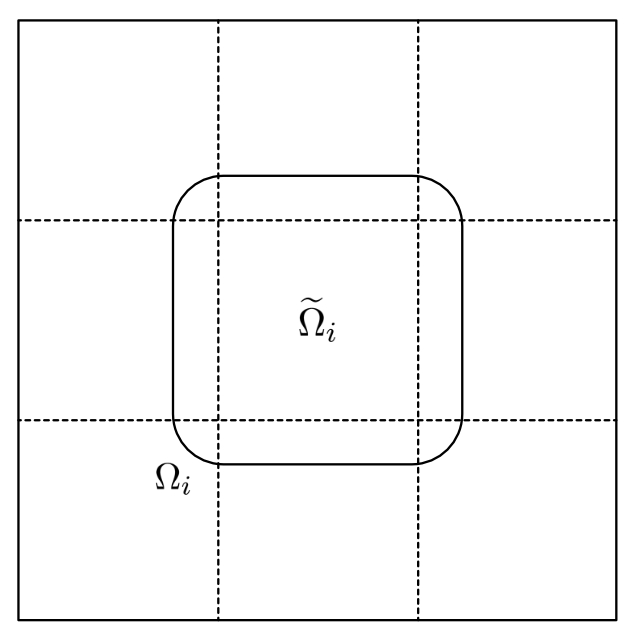
\includegraphics[width=\textwidth]{img1.jpg}
    \caption{Euclidean norm $\ell^2$}
    \label{fig11}
\end{subfigure}
\hspace{20pt}
\begin{subfigure}[b]{0.2\textwidth}
    \centering
    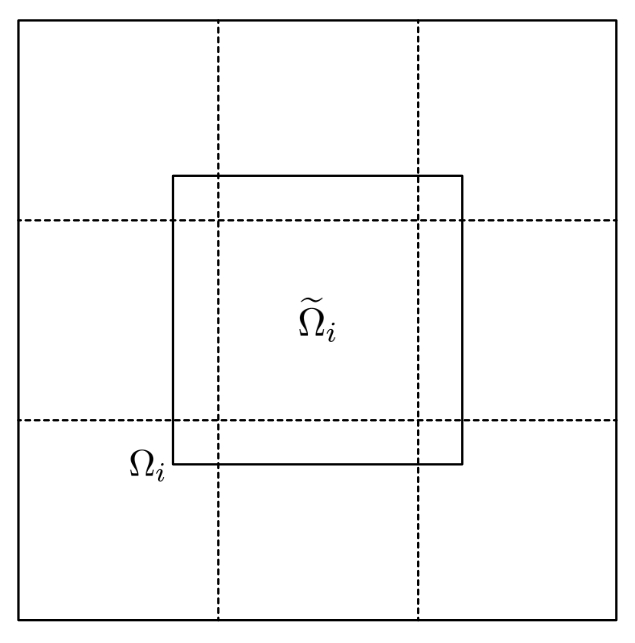
\includegraphics[width=\textwidth]{img2.jpg}
    \caption{Maximum norm $\ell^\infty$}
    \label{fig12}
\end{subfigure}
\caption{Comparison of uniform overlapping subdomains under different norms.}
\label{fig1}
\end{figure}

\noindent By definition, every point in $\Omega_i^{\delta_i}$ lies within distance $\delta_i$ of $\widetilde{\Omega}_i$, that is, 
\begin{equation*}
    \sup_{x \in \Omega_i^{\delta_{i}}} \operatorname{dist}(x, \widetilde{\Omega}_i) \leq \delta_i.
\end{equation*}
Moreover, since $\widetilde{\Omega}_i \subset \Omega_i^{\delta_{i}}$, we have 
\begin{equation*}
    \sup_{y \in \widetilde{\Omega}_i} \operatorname{dist}(y, \Omega_i^{\delta_{i}}) = 0.
\end{equation*}
It follows that the Hausdorff distance between $\Omega_i^{\delta_i}$ and $\widetilde{\Omega}_i$ satisfies
\begin{equation*}
    d_H(\Omega_i^{\delta_{i}}, \widetilde{\Omega}_i) = \max\left\{ \sup_{x \in \Omega_i^{\delta_{i}}} \operatorname{dist}(x, \widetilde{\Omega}_i), \sup_{y \in \widetilde{\Omega}_i} \operatorname{dist}(y, \Omega_i^{\delta_{i}}) \right\} \leq \delta_i,
\end{equation*}
where we consider the metric space $(M,d)$ with $M = \Omega$ and $d$ induced by the norm used in $\operatorname{dist}$. In other words, the extended subdomain $\Omega_i^{\delta_{i}}$ lies entirely within a $\delta_i$-neighborhood of $\widetilde{\Omega}_i$, while $\widetilde{\Omega}_i$ is fully contained in $\Omega_i^{\delta_{i}}$. This shows rigorously that the Hausdorff distance between the subdomain and its $\delta_i$-extension is at most $\delta_i$.

\noindent In general, the extension distance may vary across subdomains, denoted by $\delta_i$ for the $i$-th subdomain. In much of the literature, however, the extension distance is taken to be the same for all subdomains, i.e., $\delta_i = \delta$ for all $i$. The resulting decomposition is then called a \textit{uniform overlapping decomposition}. In this case, each overlapping subdomain $\Omega_i^{\delta}$ is obtained by enlarging its corresponding non-overlapping subdomain $\widetilde{\Omega}_i$ by the fixed distance $\delta$, so that
\begin{equation*}
    d_H(\widetilde{\Omega}_i, \Omega_i^{\delta}) \leq \delta.
\end{equation*}
Although $\delta$ is sometimes referred to as the \textit{overlap width}, it geometrically represents the outward extension of each subdomain. Since the overlap between neighboring subdomains results from two such extensions, $\delta$ corresponds to half of the total overlap. For this reason, we refer to $\delta$ as the \textit{uniform extension distance}.
\begin{definition}{Uniform Overlapping Domain Decomposition}{uniform_overlapping_decomposition}
Let $\{\widetilde{\Omega}_i\}_{i=1}^N$ be a non-overlapping decomposition of a bounded domain $\Omega \subset \mathbb{R}^d$. A \textbf{uniform overlapping decomposition} of $\Omega$ is a finite collection of subdomains $\{\Omega_i^{\delta}\}_{i=1}^N$ defined by
\begin{equation*}
    \Omega_i^{\delta} := \{ x \in \Omega : \operatorname{dist}(x, \widetilde{\Omega}_i) < \delta \},
\end{equation*}
where $\delta > 0$ is the \textit{uniform extension distance}.
\end{definition}
\noindent In practical applications, it is common to impose a minimal overlap between subdomains to ensure sufficient communication across interfaces. In the work of Gander and Zhao~\cite{GanderZhao2002}, the domain $\Omega$ is decomposed into $N$ nonuniform overlapping subdomains $\{\Omega_i\}_{i=1}^N$, where each subdomain is defined by
\begin{equation*}
    \Omega_i = \{ x \in \Omega : \operatorname{dist}(x, \widetilde{\Omega}_i) < \delta_i(x) \}, \qquad \delta_i(x) \geq \delta > 0, \quad x \in \Omega \setminus \widetilde{\Omega}_i,
\end{equation*}
with $\widetilde{\Gamma}_i = \partial \widetilde{\Omega}_i$ and $\Gamma_i = \partial \Omega_i$ denoting the boundaries of the non-overlapping and overlapping subdomains, respectively. They further assume that the distance between the interface boundaries satisfies
\begin{equation*}
    \operatorname{dist}(\widetilde{\Gamma}_i^{\text{int}}, \Gamma_i^{\text{int}}) \geq \delta,
\end{equation*}
so that each overlapping subdomain extends at least a distance $\delta$ beyond its corresponding non-overlapping subdomain (see Figure~\ref{fig2}). This assumption is important because, in general, a $\delta$-extension as defined above does not automatically guarantee that the Hausdorff distance between the original and extended subdomain (or their boundaries) is at least $\delta$ everywhere. Geometric constraints, such as the shape of the global domain or the arrangement of neighboring subdomains, may prevent certain regions from achieving the full extension. By explicitly assuming a minimal extension, one ensures that all subdomains overlap sufficiently, which is essential for the convergence and stability of domain decomposition methods.
\begin{figure}[H]
    \centering
    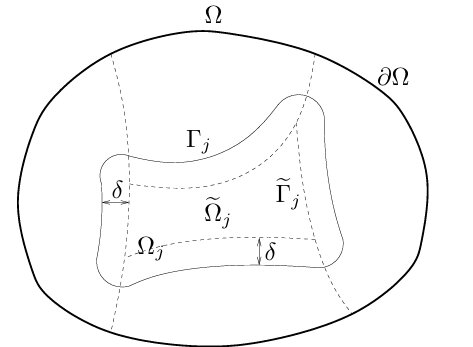
\includegraphics[width=0.3\textwidth]{delta.jpg}
    \caption{Decomposition into overlapping subdomains such that an extension of $\delta$ is guaranteed.~\cite{GanderZhao2002}}
    \label{fig2}
\end{figure}
\begin{definition}{Overlapping Domain Decomposition}{delta_overlap_decomposition}
Let $\{\widetilde{\Omega}_i\}_{i=1}^N$ be a non-overlapping decomposition of a bounded domain $\Omega \subset \mathbb{R}^d$. A collection of overlapping subdomains 
$\{\Omega_i\}_{i=1}^N$ defined by
\begin{equation*}
    \Omega_i := \{ x \in \Omega : \operatorname{dist}(x, \widetilde{\Omega}_i) < \delta_i(x) \},
\end{equation*}
where the extension function $\delta_i : \Omega \to (0,\infty)$ is a bounded, continuous function, is called a \textbf{overlapping decomposition} 
of $\Omega$ with $\delta$-extension if the \textit{minimal extension condition}
\begin{equation*}
    \operatorname{dist}(\widetilde{\Gamma}_i^{\text{int}}, \Gamma_i^{\text{int}}) \geq \delta,
\end{equation*}
is satisfied for some constant $\delta > 0$, called the \textit{minimal extension distance}.
\end{definition}
\begin{remark}
The term "minimal" does not mean that the overlap is the smallest possible. It indicates that each subdomain is extended by at least the prescribed minimal 
extension distance $\delta$ beyond its non-overlapping boundary. As a result, the minimal overlap distance, defined as the smallest overlap among all neighboring 
subdomain pairs, is at least $2\delta$. 

\vspace{6pt}
\noindent For each extended subdomain $\Omega_i$ with minimal extension distance $\delta$, the extension distances satisfy
\begin{equation*}
    \delta_i(x) \ge \operatorname{dist}(\widetilde{\Gamma}_i^{\text{int}}, \Gamma_i^{\text{int}}) \geq \delta>0, 
    \qquad 1 \leq i \leq N, \quad x \in \Omega \setminus \widetilde{\Omega}_i.
\end{equation*}
Geometrically, this means that each subdomain $\Omega_i$ contains a uniform neighborhood of width at least $\delta$ around the interior boundary of the 
corresponding subdomain $\widetilde{\Omega}_i$, guaranteeing a minimal overlap between neighboring subdomains (see Figure~\ref{fig2}).
\end{remark}

\subsubsection{Mesh-Conforming Decomposition}

Typically, theoretical results assume that $\Omega$ is a convex polytopal domain\footnote{There are two standard definitions of a polytope, and in both cases, the notion of a convex polytope is equivalent.} (convex polygonal in $\mathbb{R}^{2}$, convex polyhedral in $\mathbb{R}^{3}$). Convexity is not essential, but it simplifies analysis and guarantees that certain inequalities and estimates hold with sharp constants. For example, the Poincaré constant can be made explicit for convex domains (see Bebendorf~\cite{Bebendorf2003Poincare}). One might think that restricting to polytopal domains is limiting. In practice, however, domains with smooth or curved boundaries are often approximated by polygonal (2D) or polyhedral (3D) domains. The resulting error, called the isoparametric error, can be rigorously quantified and is considered one of the variational crimes. To avoid these issues, we assume in this paper that $\Omega \subset \mathbb{R}^{d}$ is a polytopal domain, irrespective of convexity. Note that under this assumption, the strong local Lipschitz condition is automatically satisfied, ensuring that standard Sobolev space and trace results hold.

Assuming that $\Omega \subset \mathbb{R}^{d}$ is a polytopal domain, the next step is to construct a non-overlapping decomposition of the domain, i.e., to find a finite collection of polytopal subdomains $\{\widetilde{\Omega}_{i}\}$ satisfying the conditions given in the definition above. Since we are employing the finite element method (FEM), we first generate a finite element subdivision (mesh) of the domain $\Omega$, consisting of element domains. These element domains are then grouped to form subdomains satisfying the conditions of the non-overlapping domain decomposition. Once the non-overlapping domain decomposition is constructed, an overlapping decomposition can be obtained by adding all neighbouring elements\footnote{Here, we assume vertex neighbourhoods rather than edge neighbourhoods.} to each subdomain $\widetilde{\Omega}_{i}$. Since the domain decomposition is not unique, care must be taken: one may include more elements in certain directions or extend uniformly, which affects the extension distance and, consequently, the theoretical bounds derived in the subsequent analysis.

To define a mesh-conforming decomposition of a polytopal domain, we first consider the cases $d = 1, 2$ and then extend the definition to the general case.

\begin{enumerate}[label=(\arabic*)]
\item If $d = 1$, then the domain $\Omega = (a,b)$ is an open interval. A non-overlapping decomposition of $\Omega$ into $N$ subdomains 
consists of subintervals 
\begin{equation*}
    \widetilde{\Omega}_i = (x_{i-1}, x_i),
\end{equation*}
where $x_0 = a$, $x_N = b$, and $x_i > x_{i-1}$ for $i = 1, \ldots, N$.
The partition may be uniform or non-uniform. In the uniform case,
\begin{equation*}
    x_i - x_{i-1} = h \quad \text{for } i = 1, \ldots, N,
\end{equation*}
whereas in the non-uniform case,
\begin{equation*}
    x_i - x_{i-1} = h_i, \quad \text{with } h_i \neq h_j \text{ for some } i \neq j.
\end{equation*}
As an illustrative example, one can construct a uniform overlapping decomposition of the domain is obtained by extending each subinterval by a fixed extension distance $\delta > 0$, that is,
\begin{equation*}
    \Omega_1 = (a, x_1 + \delta), \qquad \Omega_i = (x_{i-1} - \delta, x_i + \delta), \qquad \Omega_N = (x_{N-1} - \delta, b),
\end{equation*}
for $i = 2, \ldots, N-1$.

Now consider a finite element subdivision of $\Omega$, consisting of element domains $K_j$, $j = 1, \ldots, N_h$, which are closed subintervals.\footnote{In Ciarlet’s definition of a finite element, the element domain $K$ is a bounded closed set with nonempty interior and piecewise smooth boundary.} These elements form a partition of the closure of $\Omega$, i.e.,
\begin{equation*}
    \overline{\Omega} = \bigcup_{j=1}^{N_{h}}K_{j},
\end{equation*}
where each element is of the form
\begin{equation*}
    K_{j} = [y_{j-1}, y_{j}], \qquad |K_{j}| = h.\footnote{Here, $h$ denotes the size of the finite element $K_j$ and is not the same as the $h$ used above for the spacing of the non-overlapping subdomains.}
\end{equation*}
Assume that each subinterval $\widetilde{\Omega}_i$ is formed by grouping element domains, that is,
\begin{equation*}
\widetilde{\Omega}_i = \operatorname{int}\left(\bigcup_{j\in I_{i}} K_{j} \right),
\end{equation*}
where $I_{i}\subset \{1, \ldots, N_{h}\}$ are pairwise disjoint index sets satisfying
\begin{equation*}
\bigcup_{i=1}^{N} I_i = \{1, \ldots, N_h\}.
\end{equation*}
For each $i$, the overlapping index set is defined by
\begin{equation*}
    I_{i}^{\delta} = \{j \in \{1, \ldots, N_h\} : \operatorname{dist}(K_{j}, \widetilde{\Omega}_{i}) < \delta\}.
\end{equation*}
Then the overlapping subdomain $\Omega_i$ is given by
\begin{equation*}
    \Omega_i = \operatorname{int} \left(\bigcup_{j \in I_i^\delta} K_j \right).
\end{equation*}
We refer to this type of decomposition as a \textbf{mesh-conforming overlapping decomposition} of the domain $\Omega$. 
After presenting these illustrative cases, we proceed to give the general definition of an overlapping decomposition valid for arbitrary finite element partitions. 

In this construction, the extension distance is taken as $\delta = c\, h$, where $h$ denotes the mesh size of the finite element partition and $c \in \mathbb{Z}_{>0}$ specifies the number of neighboring elements to include in the overlap. 
For instance, if we wish to extend the subdomain by only one neighboring element, we take $c = 1$.

\textit{Illustrative example:} 
Consider the bounded domain $\Omega = (0,1)$, and a subdivision into $N_h = 10$ finite element domains, each of size $h = 0.1$:
\begin{equation*}
    K_1 = [0,0.1], \quad K_2 = [0.1,0.2], \quad\ldots, \quad K_{10} = [0.9,1].
\end{equation*}
Let the non-overlapping subdomains be defined by grouping elements:
\begin{align*}
    \widetilde{\Omega}_1 &= \operatorname{int}(K_1 \cup K_2 \cup K_3) = (0,0.3),\\
    \widetilde{\Omega}_2 &= \operatorname{int}(K_4 \cup K_5 \cup K_6) = (0.3,0.6),\\
    \widetilde{\Omega}_3 &= \operatorname{int}(K_7 \cup K_8 \cup K_9 \cup K_{10}) = (0.6,1).
\end{align*}
If we choose $\delta = h$, that is, we extend each subdomain by one neighboring element on each side, then the overlapping subdomains become
\begin{align*}
    \Omega_1 &= \operatorname{int}(K_1 \cup K_2 \cup K_3 \cup K_4) = (0,0.4),\\
    \Omega_2 &= \operatorname{int}(K_3 \cup K_4 \cup K_5 \cup K_6 \cup K_7) = (0.2,0.7),\\
    \Omega_3 &= \operatorname{int}(K_6 \cup K_7 \cup K_8 \cup K_9 \cup K_{10}) = (0.5,1).
\end{align*}
Here, each $\Omega_i$ is an open interval consisting of all elements of the corresponding non-overlapping subdomain together with one neighboring element on each side (whenever available). The overlap, therefore, occurs only along full elements, ensuring that the decomposition respects the finite element mesh.
\item Let $d = 2$, so that the domain $\Omega \subset \mathbb{R}^{2}$ is polygonal. Consider a finite element subdivision of $\Omega$ into element domains $K_j$, $j = 1, \ldots, N_h$. Let $\mathcal{T}_h$ denote a triangulation of $\Omega$, i.e.,  
\begin{equation*}
    \overline{\Omega} = \bigcup_{j=1}^{N_h} K_j,
\end{equation*}  
where each element $K_j \in \mathcal{T}_h$ has diameter
\begin{equation*}
    h_{K_j} := \operatorname{diam}(K_j), \quad h := \max_{K_j \in \mathcal{T}_h} h_{K_j}.
\end{equation*}  
Here, $h$ is the maximal element diameter of the mesh. We assume that $\mathcal{T}_h$ is \emph{shape-regular}, meaning there exists a constant $c > 0$, independent of $h$, such that for all $K \in \mathcal{T}_h$,  
\begin{equation*}
    \frac{h_{K_{j}}}{\rho_{K_{j}}} \leq c,
\end{equation*}  
where $\rho_{K_{j}}$ is the radius of the largest inscribed circle in $K_{j}$. Shape-regularity ensures that the elements are well-proportioned and avoids degenerate triangles.  

Suppose that each non-overlapping subdomain $\widetilde{\Omega}_i$ is obtained by grouping elements:  
\begin{equation*}
    \widetilde{\Omega}_i = \operatorname{int}\left(\bigcup_{j \in I_i} K_j \right),
\end{equation*}  
where the index sets $I_i \subset \{1, \ldots, N_h\}$ are pairwise disjoint and satisfy  
\begin{equation*}
    \bigcup_{i=1}^{N} I_i = \{1, \ldots, N_h\}.
\end{equation*}  
For each $i$, define the overlapping index set
\begin{equation*}
    I_i^\delta = \{ j \in \{1, \ldots, N_h\} : \operatorname{dist}(K_j, \widetilde{\Omega}_i) < \delta \},
\end{equation*}  
so that the corresponding overlapping subdomain is  
\begin{equation*}
    \Omega_i = \operatorname{int} \left(\bigcup_{j \in I_i^\delta} K_j \right).
\end{equation*}  
If the extension is intended to include only a single layer of neighboring elements (vertex neighbors), the extension distance can be chosen as  
\begin{equation*}
    \delta = d^{*} := \min_{K_{j}\cap K_{k} = \emptyset}\operatorname{dist}(K_{j}, K_{k}),
\end{equation*} 
where $d^{*}$ is the minimal positive separation distance between non-neighbouring elements.\footnote{Since $\mathcal{T}_h$ is a conforming triangulation, the distance $d^{*}$ is well-defined.}

\noindent Then the overlapping index set becomes  
\begin{equation*}
    I_i^{d^{*}} = \{ j \in \{1, \ldots, N_h\} : \operatorname{dist}(K_j, \widetilde{\Omega}_i) < d^{*}\},
\end{equation*}  
and the overlapping subdomain is  
\begin{equation*}
    \Omega_i = \operatorname{int} \left(\bigcup_{j \in I_i^{d^{*}}} K_j\right).
\end{equation*}  
This construction can be generalized to an arbitrary number $l$ of extension layers. Let $\Omega_i^0 := \widetilde{\Omega}_i$, and define recursively  
\begin{equation*}
    I_i^{(ld^{*})} = \{ j \in \{1, \ldots, N_h\} : \operatorname{dist}(K_j, \Omega_i^{l-1}) < d^{*}\}, \qquad \Omega_i^l = \operatorname{int} \left(\bigcup_{j \in I_i^{(ld^{*})}} K_j \right), \quad l \geq 1.
\end{equation*}  
This defines the overlapping subdomains layer by layer, with each layer including all elements within distance $d^{*}$ of the previous layer.
% \begin{figure}[H]
%     \centering
%     \includesvg[width=0.25\textwidth]{triext.svg}
%     \caption{One-layer extension of a triangular subdomain $\widetilde{\Omega}_{i}$ on an unstructured triangular mesh.}
%     \label{fig3}
% \end{figure}
As illustrated in Figure~\ref{fig3}, the overlapping subdomain $\Omega_i$ is obtained by including all elements within distance $d^{*}$ of the non-overlapping subdomain $\widetilde{\Omega}_i$, corresponding to a one-layer vertex neighborhood.
\end{enumerate}
We now state the general definition of a mesh-conforming overlapping decomposition.
\begin{definition}{Mesh-Conforming Overlapping Domain Decomposition}{meshdecomp}
    Let $\{K_j\}_{j=1}^{N_{h}}$ be a finite element subdivision of a polytopal domain $\Omega\subset \mathbb{R}^{d}$, and let
    \begin{equation*}
        \widetilde{\Omega}_{i} = \operatorname{int}\left(\bigcup_{j \in I_i} K_j \right),
    \end{equation*}
    be a non-overlapping subdomain of $\Omega$, where the index sets $I_i \subset \{1, \ldots, N_h\}$ are pairwise disjoint. A \textbf{mesh-conforming overlapping decomposition} of $\Omega$ is a finite collection of subdomains $\{\Omega_i\}$ such that
    \begin{equation*}
        \Omega_i = \operatorname{int} \left(\bigcup_{j \in I_i^\delta} K_j \right),
    \end{equation*}
    where the overlapping index set is defined by  
    \begin{equation*}
        I_{i}^{\delta} = \{j \in \{1, \ldots, N_h\} : \operatorname{dist}(K_{j}, \widetilde{\Omega}_{i}) < \delta_{i}\}.
    \end{equation*}
    and $\delta_{i} > 0$ is the extension distance.
\end{definition}
\noindent The definition is equivalent to saying that each overlapping subdomain $\Omega_i$ can be expressed as
\begin{equation*}
    \Omega_{i} = \{x\in\Omega : \operatorname{dist}(x, \widetilde{\Omega}_{i}) < \delta_{i}(x)\},
\end{equation*}
with the \textit{minimal extension condition}
\begin{equation*}
    \operatorname{dist}(\widetilde{\Gamma}_i^{\text{int}}, \Gamma_i^{\text{int}}) \geq \min_{1\leq i \leq N}\delta_{i} = : \delta,
\end{equation*}
where $\delta$ is the minimal extension distance. This equivalence also shows that a mesh-conforming overlapping decomposition is generally an 
\emph{overlapping decomposition with $\delta$-extension}. However, in certain mesh constructions, for example in structured meshes, this can 
correspond to a \emph{uniform overlapping decomposition with $\delta$-extension}, where each subdomain is extended by the same fixed distance.

\vspace{10pt}
\noindent In the paper by Maksymilian Dryja and Olof Widlund~\cite{DryjaWidlund1987}, where an additive Schwarz method for elliptic problems is presented, they choose the local extension for each subdomain, as defined in \ref{meshdecomp}, to be
\begin{equation*}
    \delta_i = \gamma \cdot \operatorname{diam}(\widetilde{\Omega}_{i}) := \gamma \cdot H_{i},
\end{equation*}
where $\gamma \in (0,1)$. This implies that the minimal extension distance is 
\begin{equation*}
    \delta = \min_{1\leq i \leq N}\delta_{i} = \gamma \cdot \min_{1\leq i \leq N}\operatorname{diam}(\widetilde{\Omega}_{i}).
\end{equation*}
Note that if we choose
\begin{equation*}
    \gamma = \dfrac{d^{*}}{\operatorname{diam}(\widetilde{\Omega}_{i})} < 1,
\end{equation*}
then the corresponding overlapping subdomain $\Omega_i$ is obtained by a one-layer extension of the triangular subdomain $\widetilde{\Omega}_i$.

\subsection{Partition of Unity}

Given an overlapping decomposition $\Omega_{1}, \ldots, \Omega_{N}$, we will employ a smooth partition of unity $\chi_{1}(x), \ldots, \chi_{N}(x)$ subordinate to these subdomains.

\begin{theorem}{Partitions of Unity, Adams \& Fournier~\cite{AdamsFournier2003}}{pou}
    Let $A$ be an arbitrary subset of $\mathbb{R}^{d}$, and let $\mathcal{O}$ be a collection of open sets covering $A$, that is, $A \subset \bigcup_{U\in \mathcal{O}}U$. Then there exists a collection $\Psi$ of functions $\psi\in C_{0}^{\infty}(\mathbb{R}^{d})$ having the following properties:
    \begin{enumerate}[label = (\roman*)]
        \item For every $\psi\in \Psi$ and every $x\in \mathbb{R}^{d}$, $0\leq \psi(x)\leq 1$.
        \item If $K\Subset A$, all but finitely many $\psi\in \Psi$ vanish identically on $K$.
        \item For every $\psi\in\Psi$ there exists $U\in \mathcal{O}$ such that $\operatorname{supp}(\psi)\subset U$.
        \item For every $x\in A$, we have $\sum_{\psi\in \Psi}\psi(x) = 1$.
    \end{enumerate}
    Such collections $\Psi$ is called a $C^{\infty}$-partition of unity for $A$ subordinate to $\mathcal{O}$.
\end{theorem}


\begin{lemma}{Partition of Unity for Overlapping Decomposition}{poud}
Let $\Omega_1, \dots, \Omega_N$ be an overlapping decomposition of a bounded domain $\Omega \subset \mathbb{R}^d$, defined as in~\ref{overdecomp}. Then there exist functions
\begin{equation*}
    \chi_i \in C^\infty(\mathbb{R}^d), \quad 1 \leq i \leq N,
\end{equation*}
satisfying the following properties:
\begin{enumerate}[label = (\roman*)]
    \item $0 \leq \chi_i(x) \leq 1 \text{ for all } x \in \mathbb{R}^d.$ 
    \item For any compact set $K \subset \Omega$, all but finitely many $\chi_i$ vanish identically on $K$.
    \item $\operatorname{supp}(\chi_i) \subset \Omega_i.$
    \item $\sum\limits_{i=1}^{N} \chi_i(x) = 1 \text{ for all } x \in \Omega.$
    \item The following gradient estimate holds:
    \begin{equation*}
        \lVert \nabla \chi_i\rVert_{L^{p}(\Omega)} \leq C(d, p, \gamma, \sigma, m)\operatorname{diam}(\widetilde{\Omega}_{i})^{\frac{d}{p}-1}.
    \end{equation*}
    Here $C(d,p,\gamma,\sigma,m) > 0$ denotes a constant depending only on
    \begin{itemize}
        \item $d$, the spatial dimension,
        \item $p$, the Lebesgue exponent,
        \item $\gamma \in (0,1)$, the overlap parameter from Definition~\ref{overdecomp},
        \item $\sigma$, the shape-regularity constant of the subdomains $\widetilde{\Omega}_i$,
        \item $m$, the maximal overlap number, i.e., the maximum number of subdomains $\Omega_i$ containing any given point in $\Omega$,
    \end{itemize}
and is independent of the mesh size $\operatorname{diam}(\widetilde{\Omega}_{i})$ and the total number of subdomains $N$.
\end{enumerate}
\end{lemma}

\begin{proof}
    Will be proved later!
\end{proof}

\begin{remark}{Partition of Unity in Waveform Relaxation}{pouowr}
In the context of Waveform Relaxation methods, the partition of unity functions $\chi_i$ are taken to be \textbf{functions of the spatial variable only}, $\chi_i = \chi_i(x)$, and do not depend on time. Each subdomain $\Omega_i$ is fixed in space, and the local solution $u_i(x,t)$ is computed iteratively over time. Consequently, there is no need for the weights $\chi_i$ to vary with time. 

\vspace{8pt}
\noindent The global solution is constructed at each time as
\begin{equation*}
    u(x,t) = \sum_{i=1}^{N} \chi_i(x)\, u_i(x,t).
\end{equation*}
Since the $\chi_i$ are time-independent, the time derivative of the global solution depends solely on the local time derivatives $\partial_t u_i$, avoiding additional terms that could complicate stability and convergence analysis. Furthermore, the spatial partition functions can be computed once and reused for all time steps, which reduces computational cost and prevents spurious temporal oscillations in the constructed solution.
\end{remark}

\subsection{Schwarz iterative algorithms}
In the literature, two important parallel Schwarz methods are commonly used: the Additive Schwarz method and the Restricted Additive Schwarz method.

\begin{enumerate}[label=(\arabic*)]
 \item Additive Schwarz method:
 \begin{align*}
    \dfrac{\partial u_{j}^{k+1}}{\partial t} &= \Delta u_{j}^{k+1} + f(x, t),\\
    u_{j}^{k+1}(x, t) &= \sum_{l\in\mathcal{N}_{j}}u_{l}^{k}(x, t), \qquad x\in \Gamma_{jl}, \,l\in \mathcal{N}_{j}, \quad 0<t<T,\\
    u_{j}^{k+1}(x, t) &= g(x, t), \qquad x\in \Gamma_{i0}, \quad 0<t<T,\\
    u_{j}^{k+1}(x, 0) &= u_{0}(x), \qquad x\in \Omega_{j}.
\end{align*}
\item Restricted Additive Schwarz method:
\begin{align*}
    \dfrac{\partial u_{j}^{k+1}}{\partial t} &= \Delta u_{j}^{k+1} + f(x, t),\\
    u_{j}^{k+1}(x, t) &= \sum_{l\in\mathcal{N}_{j}}\chi_{l}(x)u_{l}^{k}(x, t), \qquad x\in \Gamma_{jl}, \,l\in \mathcal{N}_{j}, \quad 0<t<T,\\
    u_{j}^{k+1}(x, t) &= g(x, t), \qquad x\in \Gamma_{i0}, \quad 0<t<T,\\
    u_{j}^{k+1}(x, 0) &= u_{0}(x), \qquad x\in \Omega_{j}.
\end{align*}
\end{enumerate}

\section{ROM-compatible Lifting and Weak Formulation}
Define the space
\begin{equation*}
    V_{j} = H^{1}_{0}(\Omega_{j}) = \left\{v\in H^{1}(\Omega_{j}) : v = 0 \text{ on } \partial\Omega_{j} = \Gamma_{j0}\cup\bigcup_{l\in\mathcal{N}_{j}}\Gamma_{jl}\right\}.
\end{equation*}
To enforce the nonhomogeneous boundary and interface data, we need to introduce a lifting function $l_{j}^{k+1}(\cdot, t)\in H^{1}(\Omega_{j})$ satisfying
\begin{equation*}
    l_{j}^{k+1} = 
    \begin{cases}
        u_{l}^{k} & \text{on } \Gamma_{jl},l\in \mathcal{N}_{j},\\
        g & \text{on } \Gamma_{j0},
    \end{cases}
\end{equation*}
where we should implicitly assume that\footnote{In a later remark, we will see why we need these assumptions!}
\begin{equation*}
    \left.u_{l}^{k}(\cdot, t) \right|_{\Gamma_{jl}}\in H^{1/2}(\Gamma_{jl}), \qquad \left.g(\cdot, t)\right|_{\Gamma_{jl}} \in H^{1/2}(\Gamma_{j0}), \qquad l\in \mathcal{N}_{j},
\end{equation*}
for almost every $t\in (0, T)$. By the trace theorem, the trace operator
\begin{equation*}
    \text{Tr}: W^{1, p}(\Omega_{j}) \to W^{1-\frac{1}{p}, p}(\partial\Omega_{j})
\end{equation*}
is a surjective bounded linear operator. For $p=2$, this reduces to
\begin{equation*}
    \text{Tr}: H^{1}(\Omega_{j}) \to H^{1/2}(\partial\Omega_{j}).
\end{equation*}
Moreover, the trace operator admits a bounded linear right inverse\begin{equation*}
    E_{\text{Tr}}: H^{1/2}(\partial\Omega_{j})\to H^1(\Omega_{j}),
\end{equation*}
such that
\begin{equation*}
    \text{Tr}(E_{\text{Tr}}(v)) = v, \qquad \forall v\in H^{1/2}(\partial\Omega_{j}).
\end{equation*}
Thus, defining the boundary function
\begin{equation*}
    \psi(x, t) = 
    \begin{cases}
        u_{l}^{k}(x, t) & \text{on } \Gamma_{jl}, \,l\in \mathcal{N}_{j},\\
        g(x, t) & \text{on } \Gamma_{j0},
    \end{cases}
\end{equation*}
we may choose a lifting as
\begin{equation*}
    l_{j}^{k+1}(\cdot, t) := E_{\text{Tr}}(\psi(\cdot, t)).
\end{equation*}
Note that the lifting function $l_j^{k+1}(\cdot, t)$ is not unique; any two liftings differ by an element of the space $V_{j}$.
\begin{remark}\label{mainremark}
    We must be very careful here! An extension is only possible if $\psi(\cdot, t)\in H^{1/2}(\Omega_{j})$. Let us consider the general case that encompasses all, and demonstrate that indeed we have the required regularity under the assumptions stated above. Let $\Omega_{j}\subset\mathbb{R}^{n}$ be a subdomain with neighbour set 
    \begin{equation*}
        \mathcal{N}_{j} = \{l_{1}, \ldots, l_{s_{j}}\}.
    \end{equation*}
    Suppose the boundary is originally decomposed into pieces $\Gamma_{jl}\subset\partial\Omega_{j}$ for $l\in \{0\}\cup\mathcal{N}_{j}$, which may overlap along sets of positive $(n-1)$-dimensional measure, i.e.,
    \begin{equation*}
        \Gamma_{j0} = \partial \Omega_{j} \cap \partial\Omega, \qquad \Gamma_{jl} = \left(\partial\Omega_{j}\cap\Omega_{l}\right)\setminus \Gamma_{j0}.
    \end{equation*}
    Let us consider all non-empty subsets of neighbours $\mathcal{I}\subset\mathcal{N}_{j}$, where each subset $\mathcal{I}$ corresponds to a boundary region that is shared exactly by the neighbours in $\mathcal{I}$. Then, for each $\mathcal{I}\subset\mathcal{N}_{j}$, we define
    \begin{equation*}
        \Gamma_{j}^{\mathcal{I}} := \bigcap_{l\in\mathcal{I}}\Gamma_{jl}\setminus\bigcup_{k\in\mathcal{N}_{j}\setminus\mathcal{I}}\Gamma_{jk}.
    \end{equation*}
    The set $\Gamma_{j}^{\mathcal{I}}$ is the part of $\partial\Omega_{j}$ that is shared by exactly the neighbours in $\mathcal{I}$ and no others, and the sets $\Gamma_{j}^{\mathcal{I}}$ are pairwise disjoint. 
    \begin{lemma}{}
        The sets
        \begin{equation*}
            \Gamma_{j}^{\mathcal{I}} := \bigcap_{l\in\mathcal{I}}\Gamma_{jl}\setminus\bigcup_{k\in\mathcal{N}_{j}\setminus\mathcal{I}}\Gamma_{jk}, \qquad \emptyset\neq\mathcal{I}\subset\mathcal{N}_{j}.
        \end{equation*}
        are pairwise disjoint.
    \end{lemma}
    \noindent With this definition, we obtain a disjoint decomposition of the boundary
    \begin{equation*}
        \partial\Omega_{j} = \Gamma_{j0}\cup\bigcup_{\emptyset \neq \mathcal{I}\subset\mathcal{N}_{j}}\Gamma_{j}^{\mathcal{I}}.
    \end{equation*}
    Let us now define a piecewise function on the new boundary decomposition. For each piece $\Gamma_{j}^{\mathcal{I}}$, corresponding to the subset of neighbors $\mathcal{I}\subset\mathcal{N}_{j}$, we define the boundary data as follows
    \begin{itemize}
        \item [--] \textit{Additive Schwarz:} The boundary data along a piece covered by multiple neighbors is defined as the sum of contributions from all neighbors covering that piece
        \begin{equation*}
            \psi(x, t) = \sum_{l\in\mathcal{I}}u_{l}^{k}(x, t),\qquad x\in \Gamma_{j}^{\mathcal{I}}, 
        \end{equation*}
        \item [--] \textit{Restricted Additive Schwarz:} The boundary data along a piece covered by multiple neighbors is defined as the weighted sum of contributions from all neighbors covering that piece
        \begin{equation*}
            \psi(x, t) = \sum_{l\in\mathcal{I}}w_{l}u_{l}^{k}(x, t),\qquad x\in \Gamma_{j}^{\mathcal{I}}, 
        \end{equation*}
        where the weights $0\leq w_{l} \leq 1$ satisfy the partition of unity condition
        \begin{equation*}
            \sum_{l\in \mathcal{I}}w_{l} = 1.
        \end{equation*}
    \end{itemize}
    The \textit{Gagliardo}, \textit{Aronszajn}, or \textit{Slobodeckij seminorm} of $u$ on a domain $\Omega$ is defined by
    \begin{equation*}
        [u]_{H^{1/2}(\Omega)} := \left(\iint_{\Omega\times\Omega}\dfrac{|u(x) - u(y)|^{2}}{|x-y|^{n+1}} \, dx\,dy\right)^{1/2}.
    \end{equation*}
    Then, the norm is defined by
    \begin{equation*}
        \lVert u\rVert_{H^{1/2}(\Omega)} := \left(\int_{\Omega}|u(x)|^{2}\,dx + \iint_{\Omega\times\Omega}\dfrac{|u(x) - u(y)|^{2}}{|x-y|^{n+1}} \, dx\,dy\right)^{1/2},
    \end{equation*}
    which implies that
    \begin{equation*}
         \lVert u\rVert_{H^{1/2}(\Omega)}^{2} = \lVert u\rVert^{2}_{L^{2}(\Omega)} + [u]^{2}_{H^{1/2}(\Omega)}.
    \end{equation*}
    On a manifold $\Gamma\subset\mathbb{R}^{n}$ of dimension $d = n-1$, the norm is defined as
    \begin{equation*}
         \lVert u\rVert_{H^{1/2}(\Gamma)} := \left(\int_{\Gamma}|u(x)|^{2}\,d\sigma_x + \iint_{\Gamma\times \Gamma}\dfrac{|u(x) - u(y)|^{2}}{|x-y|^{n}} \, d\sigma_x\,d\sigma_y\right)^{1/2},
    \end{equation*}
    where $d\sigma_x$ is the surface measure on $\Gamma$. Using the new decomposition, we split the squared Slobodeckij seminorm of $\psi$ on the boundary $\partial\Omega_{j}$ as
    \begin{align*}
         [\psi]_{H^{1/2}(\partial\Omega_j)}^2 &= \iint_{\Gamma_{j0} \times \Gamma_{j0}} \frac{|\psi(x, t)-\psi(y, t)|^2}{|x-y|^n} \, d\sigma_x \, d\sigma_y + \sum_{\emptyset\neq\mathcal{I}\subset\mathcal{N}_{j}} \iint_{\Gamma_j^{\mathcal{I}} \times \Gamma_j^{\mathcal{I}}} \frac{|\psi(x, t)-\psi(y, t)|^2}{|x-y|^n} \, d\sigma_x \, d\sigma_y + \\
         &\quad + 2\sum_{\emptyset\neq\mathcal{I}\subset\mathcal{N}_{j}} \iint_{\Gamma_{j0} \times \Gamma_j^{\mathcal{I}}} \frac{|\psi(x, t)-\psi(y, t)|^2}{|x-y|^n} \, d\sigma_x \, d\sigma_y + \sum_{\substack{\emptyset \neq \mathcal{I}, \mathcal{J} \subset \mathcal{N}_{j} \\ \mathcal{I} \neq \mathcal{J}}} \iint_{\Gamma_j^{\mathcal{I}} \times \Gamma_j^{\mathcal{J}}} \frac{|\psi(x, t)-\psi(y, t)|^2}{|x-y|^n} \, d\sigma_x \, d\sigma_y,
    \end{align*}
    where
    \begin{equation*}
        \psi(x, t) = 
        \begin{cases}
            \sum_{l\in\mathcal{I}}u_{l}^{k}(x, t), & x\in \Gamma_{j}^{\mathcal{I}},\\
            g(x, t), & x\in \Gamma_{j0},
        \end{cases}
    \end{equation*}
    for the Additive Schwarz method, and
    \begin{equation*}
        \psi(x, t) = 
        \begin{cases}
            \sum_{l\in\mathcal{I}}w_{l}u_{l}^{k}(x, t), & x\in \Gamma_{j}^{\mathcal{I}},\\
            g(x, t), & x\in \Gamma_{j0},
        \end{cases}
    \end{equation*}
    for the Restricted Additive Schwarz method. By the definition of the Slobodeckij seminorm on $\Gamma_{j0}$, we have
    \begin{equation*}
        [g(\cdot, t)]^{2}_{H^{1/2}(\Gamma_{j0})} = \iint_{\Gamma_{j0} \times \Gamma_{j0}} \frac{|g(x, t) - g(y, t)|^2}{|x-y|^n} \, d\sigma_x \, d\sigma_y,
    \end{equation*}
    is exactly the same as the first term. Let us now focus on the second term
    \begin{equation*}
         \sum_{\emptyset\neq\mathcal{I}\subset\mathcal{N}_{j}} \iint_{\Gamma_j^{\mathcal{I}} \times \Gamma_j^{\mathcal{I}}} \frac{|\psi(x, t)-\psi(y, t)|^2}{|x-y|^n} \, d\sigma_x \, d\sigma_y.
    \end{equation*}
    Using the definition of the boundary data and the Cauchy-Schwarz inequality, we obtain\footnote{The inequality holds for both cases considered.}
    \begin{align*}
        |\psi(x, t)-\psi(y, t)|^2 &= \left|\sum_{l\in\mathcal{I}}w_{l}u_{l}^{k}(x, t) - \sum_{l\in\mathcal{I}}w_{l}u_{l}^{k}(y, t)\right|^{2} = \left|\sum_{l\in\mathcal{I}}w_{l}\left(u_{l}^{k}(x, t) - u_{l}^{k}(y, t)\right)\right|^{2} \leq\\
        &\quad \leq \left(\sum_{l\in\mathcal{I}}w_{l}^{2}\right)\left(\sum_{l\in\mathcal{I}}\left|u_{l}^{k}(x, t) - u_{l}^{k}(y, t)\right|^{2}\right) \leq \sum_{l\in\mathcal{I}}\left|u_{l}^{k}(x, t) - u_{l}^{k}(y, t)\right|^{2},
    \end{align*}
    for $x, y\in \Gamma_{j}^{\mathcal{I}}$. Once we use this inequality, we get
    \begin{equation*}
        \sum_{\mathcal{I}\subset\mathcal{N}_{j}} \iint_{\Gamma_j^{\mathcal{I}} \times \Gamma_j^{\mathcal{I}}} \frac{|\psi(x, t)-\psi(y, t)|^2}{|x-y|^n} \, d\sigma_x \, d\sigma_y \leq \sum_{\mathcal{I}\subset\mathcal{N}_{j}} \iint_{\Gamma_j^{\mathcal{I}} \times \Gamma_j^{\mathcal{I}}} \sum_{l\in\mathcal{I}}\frac{|u_{l}^{k}(x, t) - u_{l}^{k}(y, t)|^2}{|x-y|^n} \, d\sigma_x \, d\sigma_y.
    \end{equation*}
    Because integrals are linear with respect to finite sums, and $|\mathcal{N}_{j}| < \infty$ for all $1\leq j\leq N$, the above is equivalent to
    \begin{equation*}
        \sum_{\mathcal{I}\subset\mathcal{N}_{j}} \iint_{\Gamma_j^{\mathcal{I}} \times \Gamma_j^{\mathcal{I}}} \frac{|\psi(x, t)-\psi(y, t)|^2}{|x-y|^n} \, d\sigma_x \, d\sigma_y \leq \sum_{\mathcal{I}\subset\mathcal{N}_{j}} \sum_{l\in\mathcal{I}}\iint_{\Gamma_j^{\mathcal{I}} \times \Gamma_j^{\mathcal{I}}} \frac{|u_{l}^{k}(x, t) - u_{l}^{k}(y, t)|^2}{|x-y|^n} \, d\sigma_x \, d\sigma_y.
    \end{equation*}
    Since $\Gamma_{j}^{\mathcal{I}}\subset\Gamma_{jl}$ for all $l\in \mathcal{I}$ and the integrand is nonnegative, we have
    \begin{equation*}
        \sum_{\mathcal{I}\subset\mathcal{N}_{j}} \sum_{l\in\mathcal{I}}\iint_{\Gamma_j^{\mathcal{I}} \times \Gamma_j^{\mathcal{I}}} \frac{|u_{l}^{k}(x, t) - u_{l}^{k}(y, t)|^2}{|x-y|^n} \, d\sigma_x \, d\sigma_y \leq \sum_{\mathcal{I}\subset\mathcal{N}_{j}} \sum_{l\in\mathcal{I}}\iint_{\Gamma_{jl} \times \Gamma_{jl}} \frac{|u_{l}^{k}(x, t) - u_{l}^{k}(y, t)|^2}{|x-y|^n} \, d\sigma_x \, d\sigma_y.
    \end{equation*}
    By the definition of the Slobodeckij seminorm on $\Gamma_{jl}$, we have
    \begin{equation*}
        [u_{l}^{k}]^{2}_{H^{1/2}(\Gamma_{jl})} = \iint_{\Gamma_{jl} \times \Gamma_{jl}} \frac{|u_{l}^{k}(x, t) - u_{l}^{k}(y, t)|^2}{|x-y|^n} \, d\sigma_x \, d\sigma_y,
    \end{equation*}
    which implies
    \begin{equation*}
        \sum_{\emptyset\neq\mathcal{I}\subset\mathcal{N}_{j}} \iint_{\Gamma_j^{\mathcal{I}} \times \Gamma_j^{\mathcal{I}}} \frac{|\psi(x, t)-\psi(y, t)|^2}{|x-y|^n} \, d\sigma_x \, d\sigma_y \leq \sum_{\mathcal{I}\subset\mathcal{N}_{j}} \sum_{l\in\mathcal{I}}[u_{l}^{k}(\cdot, t)]^{2}_{H^{1/2}(\Gamma_{jl})}.
    \end{equation*}


    \begin{equation*}
        \sum_{\emptyset\neq\mathcal{I}\subset\mathcal{N}_{j}} \iint_{\Gamma_{j0} \times \Gamma_j^{\mathcal{I}}} \frac{|\psi(x, t)-\psi(y, t)|^2}{|x-y|^n} \, d\sigma_x \, d\sigma_y
    \end{equation*}
    Let us now consider the second term
    \begin{equation*}
        \sum_{\mathcal{I}\neq\mathcal{J}} \iint_{\Gamma_j^{\mathcal{I}} \times \Gamma_j^{\mathcal{J}}} \frac{|\psi(x, t)-\psi(y, t)|^2}{|x-y|^n} \, d\sigma_x \, d\sigma_y.
    \end{equation*}
    Using the definition of the boundary data and the triangle inequality, we obtain
    \begin{equation*}
        |\psi(x, t) - \psi(y, t)| = \left|\sum_{l\in\mathcal{I}}w_{l}u_{l}^{k}(x, t) - \sum_{m\in\mathcal{J}}w_{m}u_{m}^{k}(y, t)\right| \leq \sum_{l\in\mathcal{I}}w_{l}|u_{l}^{k}(x, t)| + \sum_{m\in\mathcal{J}}w_{m}|u_{m}^{k}(y, t)|
    \end{equation*}
    for $x\in \Gamma_{j}^{\mathcal{I}}$, $y\in \Gamma_{j}^{\mathcal{J}}$. Using $(a+b)^{2}\leq 2a^{2} + 2b^{2}$ and the Cauchy-Schwarz inequality, we get
    \begin{align*}
        |\psi(x, t) - \psi(y, t)|^{2} &\leq \left(\sum_{l\in\mathcal{I}}w_{l}|u_{l}^{k}(x, t)| + \sum_{m\in\mathcal{J}}w_{m}|u_{m}^{k}(y, t)|\right)^{2} \leq \\
        &\leq 2\left(\sum_{l\in\mathcal{I}}w_{l}|u_{l}^{k}(x, t)|\right)^{2} + 2\left(\sum_{m\in\mathcal{J}}w_{m}|u_{m}^{k}(x, t)|\right)^{2}\leq\\
        &\leq 2\left(\sum_{l\in\mathcal{I}}w_{l}^{2}\right)\left(\sum_{l\in\mathcal{I}}|u_{l}^{k}(x, t)|^{2}\right) + 2\left(\sum_{m\in\mathcal{J}}w_{m}^{2}\right)\left(\sum_{m\in\mathcal{J}}|u_{m}^{k}(x, t)|^{2}\right)\leq\\
        &\leq 2\sum_{l\in\mathcal{I}}|u_{l}^{k}(x, t)|^{2} + 2\sum_{m\in\mathcal{J}}|u_{m}^{k}(x, t)|^{2}.
    \end{align*}
    Using this inequality, we arrive at
    \begin{align*}
        \iint_{\Gamma_j^{\mathcal{I}} \times \Gamma_j^{\mathcal{J}}} \frac{|\psi(x, t)-\psi(y, t)|^2}{|x-y|^n} \, d\sigma_x \, d\sigma_y &\leq 2\sum_{l\in\mathcal{I}}\int_{\Gamma_j^{\mathcal{I}}}|u_{l}^{k}(x, t)|^{2} \int_{\Gamma_j^{\mathcal{J}}}\dfrac{1}{|x-y|^n}\,d\sigma_y\,d\sigma_x + \\
        &\quad +2\sum_{m\in\mathcal{J}}\int_{\Gamma_j^{\mathcal{J}}}|u_{m}^{k}(x, t)|^{2} \int_{\Gamma_j^{\mathcal{I}}}\dfrac{1}{|x-y|^n}\,d\sigma_x\,d\sigma_y.
    \end{align*}
    
    Considering the $H^{1/2}$ norm definition on $\partial\Omega_{j}$, we also need to consider
    \begin{align*}
         \lVert \psi(\cdot, t)\rVert^{2}_{L^{2}(\partial\Omega_{j})} &= \sum_{\mathcal{I}\subset\mathcal{N}_{j}}\int_{\Gamma_{j}^{\mathcal{I}}}|\psi(x, t)|^{2}\, d\sigma_{x} = \sum_{\mathcal{I}\subset\mathcal{N}_{j}}\int_{\Gamma_{j}^{\mathcal{I}}}\left|\sum_{l\in\mathcal{I}}w_{l}u_{l}^{k}(x, t)\right|^{2}\, d\sigma_{x}\leq\\
         &\quad \leq \sum_{\mathcal{I}\subset\mathcal{N}_{j}}\left(\sum_{l\in\mathcal{I}}w_{l}^{2}\right)\int_{\Gamma_{j}^{\mathcal{I}}}\sum_{l\in\mathcal{I}}\left|u_{l}^{k}(x, t)\right|^{2}\, d\sigma_{x} \leq \sum_{\mathcal{I}\subset\mathcal{N}_{j}}\int_{\Gamma_{j}^{\mathcal{I}}}\sum_{l\in\mathcal{I}}\left|u_{l}^{k}(x, t)\right|^{2}\, d\sigma_{x}\leq\\
         &\quad \leq\sum_{\mathcal{I}\subset\mathcal{N}_{j}}\sum_{l\in\mathcal{I}}\int_{\Gamma_{j}^{\mathcal{I}}}\left|u_{l}^{k}(x, t)\right|^{2}\, d\sigma_{x} \leq \sum_{\mathcal{I}\subset\mathcal{N}_{j}}\sum_{l\in\mathcal{I}}\int_{\Gamma_{jl}}\left|u_{l}^{k}(x, t)\right|^{2}\, d\sigma_{x} = \sum_{\mathcal{I}\subset\mathcal{N}_{j}}\sum_{l\in\mathcal{I}}\lVert u_{l}^{k}(\cdot, t)\rVert^{2}_{L^{2}(\Gamma_{jl})}.
    \end{align*}
    If we combine all the results obtained, we have 
    \begin{equation*}
         \lVert \psi(\cdot, t)\rVert_{H^{1/2}(\partial\Omega_{j})}^{2} = \lVert \psi(\cdot, t)\rVert^{2}_{L^{2}(\partial\Omega_{j})} + [\psi(\cdot, t)]^{2}_{H^{1/2}(\partial\Omega_{j})} \leq \sum_{\mathcal{I}\subset\mathcal{N}_{j}}\sum_{l\in\mathcal{I}}\left(\lVert u_{l}^{k}(\cdot, t)\rVert^{2}_{L^{2}(\Gamma_{jl})} + [u_{l}^{k}(\cdot, t)]^{2}_{H^{1/2}(\Gamma_{jl})}\right),         
    \end{equation*}
    or equivalently
    \begin{equation*}
        \lVert \psi(\cdot, t)\rVert_{H^{1/2}(\partial\Omega_{j})}^{2} \leq \sum_{\mathcal{I}\subset\mathcal{N}_{j}}\sum_{l\in\mathcal{I}}\lVert u_{l}^{k}(\cdot, t)\rVert_{H^{1/2}(\Gamma_{jl})}^{2}.
    \end{equation*}
    Now, we can clearly see that 
    \begin{equation*}
        \left.u_{l}^{k}(\cdot, t)\right|_{\Gamma_{jl}} \in H^{1/2}(\Gamma_{jl}) \implies \psi(\cdot, t)\in H^{1/2}(\partial\Omega_{j}).
    \end{equation*}
    Before proceeding, one should note that in the formulation we ignore the case where one part of the boundary is $\Gamma_{i0}$, as well as its contribution to the boundary data function $\psi(x, t)$. For this case, we explicitly state the definition of the interface boundary, i.e.,
    \begin{equation*}
        \Gamma_{j0} = \partial \Omega_{j} \cap \partial\Omega, \qquad \Gamma_{jl} = \left(\partial\Omega_{j}\cap\Omega_{l}\right)\setminus \Gamma_{j0}.
    \end{equation*}
    Thus, the decomposition of the boundary up to measure zero becomes
    \begin{equation*}
        \partial\Omega_{j} = \Gamma_{j0} \cup \bigcup_{\emptyset \neq \mathcal{I}\subset\mathcal{N}_{j}}\Gamma_{j}^{\mathcal{I}},
    \end{equation*}
    and the squared Slobodeckij seminorm of $\psi$ on the boundary $\partial\Omega_{j}$ reduces to
    \begin{equation*}
         [\psi]_{H^{1/2}(\partial\Omega_j)}^2 = \iint_{\Gamma_{j0} \times \Gamma_{j0}} \frac{|\psi(x, t)-\psi(y, t)|^2}{|x-y|^n} \, d\sigma_x \, d\sigma_y + \sum_{\mathcal{I}\subset\mathcal{N}_{j}} \iint_{\Gamma_j^{\mathcal{I}} \times \Gamma_j^{\mathcal{I}}} \frac{|\psi(x, t)-\psi(y, t)|^2}{|x-y|^n} \, d\sigma_x \, d\sigma_y,
    \end{equation*}
    where
    \begin{equation*}
        \psi(x, t) = 
        \begin{cases}
            \sum_{l\in\mathcal{I}}u_{l}^{k}(x, t), & x\in \Gamma_{j}^{\mathcal{I}},\\
            g(x, t), & x\in \Gamma_{j0},
        \end{cases}
    \end{equation*}
    for the Additive Schwarz method, and
    \begin{equation*}
        \psi(x, t) = 
        \begin{cases}
            \sum_{l\in\mathcal{I}}w_{l}u_{l}^{k}(x, t), & x\in \Gamma_{j}^{\mathcal{I}},\\
            g(x, t), & x\in \Gamma_{j0},
        \end{cases}
    \end{equation*}
    for the Restricted Additive Schwarz method. By the definition of the Slobodeckij seminorm on $\Gamma_{j0}$, we have
    \begin{equation*}
        [g(\cdot, t)]^{2}_{H^{1/2}(\Gamma_{j0})} = \iint_{\Gamma_{j0} \times \Gamma_{j0}} \frac{|g(x, t) - g(y, t)|^2}{|x-y|^n} \, d\sigma_x \, d\sigma_y,
    \end{equation*}
    which implies that
    \begin{equation*}
        \lVert \psi(\cdot, t)\rVert_{H^{1/2}(\partial\Omega_{j})}^{2} \leq \lVert g(\cdot, t)\rVert_{H^{1/2}(\Gamma_{j0})}^{2} + \sum_{\mathcal{I}\subset\mathcal{N}_{j}}\sum_{l\in\mathcal{I}}\lVert u_{l}^{k}(\cdot, t)\rVert_{H^{1/2}(\Gamma_{jl})}^{2}.
    \end{equation*}
    Here, we can see the general assumptions required for $\psi(\cdot, t)$ to be in $H^{1/2}(\partial\Omega_{j})$, i.e.,
    \begin{equation*}
        \left.u_{l}^{k}(\cdot, t)\right|_{\Gamma_{jl}} \in H^{1/2}(\Gamma_{jl}), \qquad \left.g(\cdot, t)\right|_{\Gamma_{j0}} \in H^{1/2}(\Gamma_{j0}) \implies \psi(\cdot, t)\in H^{1/2}(\partial\Omega_{j}),
    \end{equation*}
    which was already stated on the first page.
\end{remark}

\begin{definition}{Dirichlet-type transmission operator}{dt}
    Let $\Gamma_{jl} \subset \Omega_l$ denote the interface between subdomains $j$ and $l$, which is an interior Lipschitz manifold of codimension one. We define the \emph{Dirichlet-type transmission operator} $\mathcal{T}_{jl}: H^1(\Omega_l) \to H^{1/2}(\Gamma_{jl})$, which extracts the solution values on $\Gamma_{jl}$ for use as boundary data in the overlapping waveform relaxation iteration. For a function $u_l^k \in H^1(\Omega_l)$, the operator is defined as
    \begin{equation*}
        \mathcal{T}_{jl} u_l^k := u_l^k|_{\Gamma_{jl}}.
    \end{equation*}
\end{definition}
This definition is well-posed because $\Gamma_{jl}$ is a Lipschitz manifold of codimension one. By the \emph{trace/restriction theorem} for interior manifolds\footnote{I could not find a reference where this result is stated explicitly; however, assuming a Lipschitz interface is sufficient. Indeed, one can use a local chart to map the curved interface to a flat $(n-1)$-dimensional hyperplane, obtain a local trace inequality, and then combine the estimates using a partition of unity subordinate to the covering.}, there exists a bounded linear restriction operator
\begin{equation*}
    \text{Tr}_{\Gamma_{jl}}: H^1(\Omega_l) \to H^{1/2}(\Gamma_{jl}),
\end{equation*}
which ensures that
\begin{equation*}
    u_l^k|_{\Gamma_{jl}} \in H^{1/2}(\Gamma_{jl}).
\end{equation*}
Hence, the Dirichlet-type transmission operator $\mathcal{T}_{jl}$ is well-defined and provides interface data with sufficient regularity to impose as Dirichlet boundary conditions on subdomain $j$. In other words, the assumptions we made for the existence of a lifting function are not restrictive and indeed direct consequences of the assumptions $u_l^k \in H^1(\Omega_l)$ for $1\leq l \leq N$, i.e.,
\begin{equation*}
    u_l^k \in H^1(\Omega_l) \implies \left.u_l^k\right|_{\Gamma_{jl}} \in H^{1/2}(\Gamma_{jl}).
\end{equation*}
For the Dirichlet boundary function $g(x, t)$, it is enough to assume $g(\cdot, t)\in H^{1/2}(\partial\Omega)$ since $\partial\Omega = \cup_{1\leq i\leq N}\Gamma_{i0}$.
\begin{remark}
   In more general domain decomposition methods, transmission operators may involve Neumann or Robin-type conditions. In the present Dirichlet-type setting, $\mathcal{T}_{jl}$ coincides with the restriction of $u_l^k$ to the interface $\Gamma_{jl}$. 
\end{remark}
\noindent Considering the Remark~\ref{mainremark}, one can rewrite the waveform relaxation subproblem for the subdomain $\Omega_{j}$ as
\begin{align*}
    \dfrac{\partial u_{j}^{k+1}}{\partial t} &= \Delta u_{j}^{k+1} + f(x, t),\\
    u_{j}^{k+1}(x, t) &= \psi_{j}^{k}(x, t), \qquad x\in \partial\Omega_{j}, \quad 0<t<T,\\
    u_{j}^{k+1}(x, 0) &= u_{0}(x), \qquad x\in \Omega_{j},
\end{align*}
where
\begin{equation*}
    \psi_{j}^{k}(x, t) = 
    \begin{cases}
        \sum_{l\in\mathcal{I}}u_{l}^{k}(x, t), & x\in \Gamma_{j}^{\mathcal{I}},\\
        g(x, t), & x\in \Gamma_{j0},
    \end{cases}
\end{equation*}
for the Additive Schwarz method, and
\begin{equation*}
    \psi_{j}^{k}(x, t) = 
    \begin{cases}
        \sum_{l\in\mathcal{I}}w_{l}u_{l}^{k}(x, t), & x\in \Gamma_{j}^{\mathcal{I}},\\
        g(x, t), & x\in \Gamma_{j0},
    \end{cases}
\end{equation*}
for the Restricted Additive Schwarz method. 
\begin{theorem}{}
Let $\Omega_j \subset \mathbb{R}^n$ be a subdomain with Lipschitz boundary $\partial\Omega_j$, and let $\Gamma_{jl} \subset \Omega_l$ for $l \in \mathcal{N}_j$ be the interfaces, assumed to be Lipschitz $(n-1)$-dimensional manifolds. Assume the Dirichlet boundary function $g(\cdot, t) \in H^{1/2}(\partial\Omega)$ and $u_l^k(\cdot, t) \in H^{1}(\Omega_{l})$ for all $l \in \mathcal{N}_j$ for almost every $t \in (0,T)$. Define the boundary decomposition
\[
\partial\Omega_j = \Gamma_{j0} \cup \bigcup_{\emptyset \neq \mathcal{I} \subset \mathcal{N}_j} \Gamma_j^{\mathcal{I}},
\]
where $\Gamma_{j0} = \partial \Omega_j \cap \partial \Omega$ and, for each $\emptyset \neq \mathcal{I} \subset \mathcal{N}_j$,
\[
\Gamma_j^{\mathcal{I}} := \bigcap_{l \in \mathcal{I}} \Gamma_{jl} \;\setminus\; \bigcup_{k \in \mathcal{N}_j \setminus \mathcal{I}} \Gamma_{jk},
\]
where the sets $\Gamma_j^{\mathcal{I}}$ are disjoint up to measure zero. Define the piecewise boundary function $\psi(\cdot, t) : \partial \Omega_j \to \mathbb{R}$ by
\[
\psi(\cdot, t) =
\begin{cases}
\displaystyle \sum_{l \in \mathcal{I}} u_l^k(\cdot, t), & x \in \Gamma_j^{\mathcal{I}} \text{ (Additive Schwarz)}, \\[1.5em]
\displaystyle \sum_{l \in \mathcal{I}} w_l \, u_l^k(\cdot, t), \quad \sum_{l \in \mathcal{I}} w_l = 1, \; 0 \leq w_l \leq 1, & x \in \Gamma_j^{\mathcal{I}} \text{ (Restricted Additive Schwarz)}, \\[1em]
g(\cdot, t), & x \in \Gamma_{j0}.
\end{cases}
\]
Then there exists a lifting function
\[
l_j^{k+1}(\cdot, t) \in H^1(\Omega_j)
\]
satisfying
\[
l_j^{k+1}(\cdot, t)\big|_{\partial \Omega_j} = \psi(\cdot, t),
\]
with the norm bound
\[
\lVert l_j^{k+1}(\cdot, t) \rVert_{H^1(\Omega_j)} \leq C \, \lVert \psi(\cdot, t) \rVert_{H^{1/2}(\partial \Omega_j)},
\]
where $C>0$ depends only on $\Omega_j$. Consequently, the overlapping waveform relaxation subproblem on $\Omega_j$ with nonhomogeneous Dirichlet boundary data
\[
u_j^{k+1}\big|_{\partial \Omega_j} = \psi(\cdot, t)
\]
is well-posed in the weak sense.
\end{theorem}
\begin{remark}[You may ignore this!]
    Recall the inequality
    \begin{equation*}
        \lVert \psi(\cdot, t)\rVert_{H^{1/2}(\partial\Omega_{j})}^{2} \leq \lVert g(\cdot, t)\rVert_{H^{1/2}(\Gamma_{j0})}^{2} + \hat{C}\sum_{l\in\mathcal{N}_{j}}\lVert u_{l}^{k}(\cdot, t)\rVert_{H^{1/2}(\Gamma_{jl})}^{2},
    \end{equation*}
    with some constant $\hat{C} > 0$. Combining this with the estimate from the theorem, yields
    \begin{equation*}
        \lVert l_j^{k+1}(\cdot, t) \rVert^{2}_{H^1(\Omega_j)} \leq C^{2} \, \lVert \psi(\cdot, t) \rVert^{2}_{H^{1/2}(\partial \Omega_j)} \leq c_{1}\lVert g(\cdot, t)\rVert_{H^{1/2}(\Gamma_{j0})}^{2} + c_{2}\sum_{l\in\mathcal{N}_{j}}\lVert u_{l}^{k}(\cdot, t)\rVert_{H^{1/2}(\Gamma_{jl})}^{2},
    \end{equation*}
    for some constants $c_{1}, c_{2} > 0$. Moreover, using the continuity of the trace operator, we obtain
    \begin{equation*}
        \lVert l_j^{k+1}(\cdot, t) \rVert^{2}_{H^1(\Omega_j)} \leq \Tilde{c}_{1}\lVert g(\cdot, t)\rVert_{H^{1}(\Omega)}^{2} + \Tilde{c}_{2}\sum_{l\in\mathcal{N}_{j}}\lVert u_{l}^{k}(\cdot, t)\rVert_{H^{1}(\Omega_{l})}^{2},
    \end{equation*}
    with constants $\tilde{c}_{1}, \tilde{c}_{2} > 0$.
\end{remark}
This theorem is very important as it gives the regularity assumptions for the existence of a lifting function. Then, we can decompose the solution as
\begin{equation*}
    u_{j}^{k+1} = w^{k+1}_{j} + l_{j}^{k+1}, \qquad w^{k+1}_{j}\in V_{j}.
\end{equation*}
Let us substitute this form into the equation.
\begin{equation*}
    \dfrac{\partial \left(w^{k+1}_{j} + l_{j}^{k+1}\right)}{\partial t} = \Delta \left(w^{k+1}_{j} + l_{j}^{k+1}\right) + f(x, t),
\end{equation*}
or equivalently
\begin{equation*}
    \dfrac{\partial w^{k+1}_{j}}{\partial t} - \Delta w^{k+1}_{j} = f(x, t) + \Delta l_{j}^{k+1} - \dfrac{\partial l_{j}^{k+1}}{\partial t}.
\end{equation*}
Take an arbitrary test function $v\in V_{j}$ and multiply the equation by $v$ and integrate over $\Omega_{j}$:
\begin{equation*}
    \int_{\Omega_{j}}\partial_{t} w^{k+1}_{j} v \,dx - \int_{\Omega_{j}} \Delta w^{k+1}_{j}v \,dx = \int_{\Omega_{j}} f(x, t)v \,dx + \int_{\Omega_{j}} \Delta l_{j}^{k+1} v \,dx - \int_{\Omega_{j}}\partial_{t} l_{j}^{k+1}v \,dx.
\end{equation*}
Once we use Green's first identity and the fact that the test function $v$ vanishes on the boundary, the weak formulation reads as: for almost $t\in (0, T)$, find $w_{j}^{k+1}(t)\in V_{j}$ such that
\begin{equation*}
    \left(\partial_{t} w_{j}^{k+1}, v\right)_{\Omega_{j}} + \left(\nabla w_{j}^{k+1}, \nabla v\right)_{\Omega_{j}} = \left(f, v\right)_{\Omega_{j}} - \left(\partial_{t} l_{j}^{k+1}, v\right)_{\Omega_{j}} - \left(\nabla l_{j}^{k+1}, \nabla v\right)_{\Omega_{j}}, \quad\forall v\in V_{j},
\end{equation*}
with initial condition
\begin{equation*}
    w^{k+1}_{j}(x, 0) = u_{0}(x) - l_{j}^{k+1}(x, 0).
\end{equation*}
We are not done! Recall that the lifting is not unique. If we choose $l_j^{k+1}$ to be a \emph{harmonic lifting}, i.e., it solves the problem 
\begin{align*}
    -\Delta l_j^{k+1}(x, t) &= 0 \quad x\in\Omega_j,\\
    l_j^{k+1}(x, t) &= \psi_{j}^{k}(x, t) \quad x\in \partial\Omega_j,
\end{align*}
for each $t\in (0, T)$, then this minimizes the Dirichlet energy in $\Omega_j$ and leads to a simpler weak formulation. We decompose the solution as
\begin{equation*}
    u_{j}^{k+1} = w^{k+1}_{j} + l_{j}^{k+1}, \qquad w^{k+1}_{j}\in V_{j},
\end{equation*}
where $l_j^{k+1} $ is a harmonic lifting. Substituting into the heat equation and using the harmonic property $\Delta l_j^{k+1} = 0$ yields
\begin{equation*}
    \partial_t w_j^{k+1} - \Delta w_j^{k+1} = f(x, t) - \partial_t l_j^{k+1}.
\end{equation*}
Taking $v \in V_j$ as test function and integrating over $\Omega_j$, the weak formulation reads: for almost $t \in (0,T)$, find $w_j^{k+1}(t) \in V_j$ such that
\begin{equation*}
    \left(\partial_t w_j^{k+1}, v\right)_{\Omega_j} + \left(\nabla w_j^{k+1}, \nabla v\right)_{\Omega_j} = (f, v)_{\Omega_j} - \left(\partial_t l_j^{k+1}, v\right)_{\Omega_j}, \quad \forall v \in V_j,
\end{equation*}
with initial condition
\begin{equation*}
    w_j^{k+1}(x,0) = u_0(x) - l_j^{k+1}(x,0).
\end{equation*}
\begin{remark}
    Choosing a harmonic lifting simplifies both the weak formulation and the numerical implementation. Moreover, if the boundary conditions fully determine the lifting, it is unique, eliminating the non-uniqueness present in general $H^1$ liftings.
\end{remark} 
\noindent Let $V_{j, r}\subset V_{j}$ be a finite-dimensional reduced space with $r = \dim(V_{j, r})$, and let $\{\phi_{i}\}_{i=1}^{r}$ be a basis of $V_{j, r}$. In the reduced formulation, the reduction is applied only to the homogeneous part of the solution. Accordingly, we expand only the homogeneous component $w^{k+1}_{j}$ in the reduced basis:
\begin{equation*}
    w^{k+1}_{j, r}(x, t) = \sum_{i=1}^{r}\alpha^{k+1}_{i}(t)\phi_{i}(x).
\end{equation*}
The function $w^{k+1}_{j,r}$ is referred to as the reduced (or reconstructed) approximation of $w_{j}^{k+1}$. Although it is obtained through a reduced expansion, it is a function defined on $\Omega_j$ and belongs to the reduced space $V_{j,r}=\operatorname{span}\{\phi_1,\dots,\phi_r\}$. Since $V_{j,r}\subset V_j$, $w^{k+1}_{j,r}$ is naturally identified as an element of $V_j$. This identification allows us to compare the reduced and full solutions directly and to define the error $e_{j,r}^{k+1}=w_{j}^{k+1}-w_{j,r}^{k+1} + \delta_{j}^{k+1}$ in $V_j$. From a numerical perspective, the term "reconstructed" emphasizes that the function $w^{k+1}_{j,r}$ is obtained by combining the ROM coefficients $\alpha^{k+1}_i(t)$ with the basis functions $\phi_i(x)$ to form a function in the full domain. 

\vspace{10pt}
\noindent Then, the ROM weak formulation reads: for almost $t \in (0,T)$, find $w_{j, r}^{k+1}(t) \in V_{j, r}$ such that
\begin{equation*}
    \left(\partial_{t} w_{j, r}^{k+1}, v_{r}\right)_{\Omega_{j}} + \left(\nabla w_{j, r}^{k+1}, \nabla v_{r}\right)_{\Omega_{j}} = \left(f, v_{r}\right)_{\Omega_{j}} - \left(\partial_{t} l_{j}^{k+1}, v_{r}\right)_{\Omega_{j}} - \left(\nabla l_{j}^{k+1}, \nabla v_{r}\right)_{\Omega_{j}}, \quad\forall v_{r}\in V_{j, r},
\end{equation*}
This formulation assumes that the lifting $l_j^{k+1}(x,t)$ is known for each iteration $k+1$. However, by definition, $l_j^{k+1}$ depends on the neighbouring subdomain solution $u_l^k$, which is only available once the previous iteration has been solved. Consequently, in a fully reduced-order setting, $l_j^{k+1}$ cannot be constructed from FOM solutions at each iteration. To obtain a self-contained ROM iteration, the lifting must be defined solely from reduced solutions or their projections, ensuring that the reduced problem can be solved independently of FOM computations. The remedy is to make the lifting fully compatible with the reduced-order framework, so that the ROM can be solved without access to FOM solutions at each iteration. 

A straightforward approach is to take the neighboring reduced solution(s) $u_{l, r}^k \in V_{l,r}$, compute its trace on the interface $\Gamma_{jl}$, and then extend this trace to the subdomain volume to construct a lifting function $l_{j, r}^{k+1}$. The extension can be done using a simple (nodal) lifting or a more sophisticated approach such as a harmonic lifting. In either case, the lifting depends solely on reduced quantities, ensuring that the reduced-order iteration is independent of the full-order solution. I refer to this procedure as a \emph{reduced-order compatible lifting}. Let us define the reduced boundary function\footnote{Please note that this definition is not correct for the general case and must be modified depending on the Schwarz method used. To see modified versions, please refer to the FOM version above, or see below.}
\begin{equation*}
    \psi_{j, r}^{k}(x, t) = 
    \begin{cases}
        u_{l, r}^{k}(x, t) & x\in \Gamma_{jl},\, l\in \mathcal{N}_{j},\\
        g(x, t) & x\in \Gamma_{j0}.
    \end{cases}
\end{equation*}
To be more precise, a ROM-compatible lifting function $l_{j, r}^{k+1}(\cdot, t)\in H^{1}(\Omega_{j})$ is defined by
\begin{equation*}
    l_{j, r}^{k+1}(\cdot, t) := E_{\text{Tr}}(\psi_{j, r}^{k}(\cdot, t)),
\end{equation*}
where the extension is made into the subdomain interior using a suitable lifting procedure. By suitable lifting, we mean any method that defines a function in the interior of the subdomain that matches the prescribed boundary/interface values. There are two common choices we consider in this paper:\footnote{The numerical implementation will be discussed in detail in the next section.}
\begin{itemize}
    \item[--] \textit{Nodal (or simple) lifting:} the interior values are set to zero, so the lifting is nonzero only near the interface. This approach is computationally inexpensive and easy to implement. Also, we do not solve a PDE for $l^{k+1}_{j, r}$, and it does not satisfy the original weak form exactly. It is a numerical approximation: it enforces the boundary at the nodes only, not everywhere along $\partial\Omega_{j}$.
    \item[--] \textit{Harmonic lifting:} the interior distribution is computed by solving a Laplace problem in the subdomain, 
    \begin{align*}
        -\Delta l^{k+1}_{j, r}(x, t) &= 0, \quad x\in\Omega_j,\\
        l_{j, r}^{k+1}(x, t) &= \psi_{j, r}^{k}(x, t), \quad x\in \partial\Omega_j,
    \end{align*}
    for each $t\in (0, T)$, which produces a smooth extension of the boundary/interface values into the interior. This approach is slightly more expensive but may improve the accuracy of the reduced solution near interfaces.
\end{itemize}
The choice of lifting affects the reduced weak formulation through additional terms involving the lifting. For nodal lifting, both mass and stiffness contributions appear, whereas for harmonic lifting, the stiffness contribution vanishes, leading to a simplified reduced formulation. The general ROM weak formulation reads: for almost $t \in (0,T)$, find $w_{j, r}^{k+1}(t) \in V_{j, r}$ such that
\begin{equation*}
    \left(\partial_{t} w_{j, r}^{k+1}, v_{r}\right)_{\Omega_{j}} + \left(\nabla w_{j, r}^{k+1}, \nabla v_{r}\right)_{\Omega_{j}} = \left(f, v_{r}\right)_{\Omega_{j}} - \left(\partial_{t} l_{j, r}^{k+1}, v_{r}\right)_{\Omega_{j}} - \left(\nabla l_{j, r}^{k+1}, \nabla v_{r}\right)_{\Omega_{j}}, \quad\forall v_{r}\in V_{j, r}.
\end{equation*}
\noindent The reduced solution is then written as
\begin{equation*}
    u_{j, r}^{k+1}(x, t) = w^{k+1}_{j, r}(x, t) + l_{j, r}^{k+1}(x, t), \qquad w^{k+1}_{j, r}\in V_{j, r}.
\end{equation*}
\begin{definition}{Projection operator}{po}
    The \textit{projection operator} $P_{j, r}: V_{j} \to V_{j, r}$ is defined by
    \begin{equation*}
        P_{j,r} u := \arg\min_{v_r \in V_{j,r}} \lVert u - v_r \rVert_{V_j},
    \end{equation*}
    i.e., for any $u \in V_j$, $P_{j,r} u$ is the best approximation of $u$ in the reduced space $V_{j,r}$ with respect to the norm $\|\cdot\|_{V_j}$. The projection of $w_j^{k+1}\in V_{j}$ onto $V_{j,r}$ can be written as
    \begin{equation*}
        P_{j,r} w_j^{k+1} = \sum_{i=1}^r \alpha_i^{k+1} \phi_i,
    \end{equation*}
    where the coefficients $\alpha^{k+1} = \left(\alpha_1^{k+1},\dots,\alpha_r^{k+1}\right)^{T}$ are determined by the best-approximation property
    \begin{equation*}
        \lVert w_j^{k+1} - P_{j,r} w_j^{k+1} \rVert_{V_j} = \min_{v_r \in V_{j,r}} \lVert w_j^{k+1} - v_r \rVert_{V_j}.
    \end{equation*}
    Equivalently, $P_{j,r} w_j^{k+1}$ is characterized by the \textit{orthogonality condition}
    \begin{equation*}
        \left(w_j^{k+1} - P_{j,r} w_j^{k+1}, v_r \right)_{V_j} = 0, \qquad \forall v_r \in V_{j,r},
    \end{equation*}
    where $(\cdot,\cdot)_{V_j}$ denotes the inner product associated with the norm $\lVert\cdot\rVert_{V_j}$. In terms of the basis $\{\phi_i\}_{i=1}^r$, this condition leads to the linear system
    \begin{equation*}
        \sum_{i=1}^r \left(\phi_i,\phi_l\right)_{V_j} \alpha_i^{k+1} = \left(w_j^{k+1},\phi_l\right)_{V_j}, \qquad l = 1,\ldots,r.
    \end{equation*}
\end{definition}
\noindent The total error between the full and reduced solutions is defined by
\begin{equation*}
    e_{j, r}^{k+1}(\cdot, t) : = u_{j}^{k+1}(\cdot, t) - u_{j, r}^{k+1}(\cdot, t) = w_{j}^{k+1}(\cdot, t) - w_{j, r}^{k+1}(\cdot, t) + l_{j}^{k+1} - l_{j, r}^{k+1}\in H^{1}(\Omega_{j}).
\end{equation*}
To compare the reduced and full solutions in a compatible way, we introduce the projection of the full homogeneous solution onto the reduced space, $P_{j,r} w_j^{k+1} \in V_{j,r}$, and define the total error as
\begin{equation*}
    e_{j, r}^{k+1} = \underbrace{\left(w_{j}^{k+1} - P_{j,r}w_{j}^{k+1}\right)}_{\text{projection error }\in\, V_{j}} + \underbrace{\left(P_{j,r}w_{j}^{k+1} - w_{j, r}^{k+1}\right)}_{\text{ROM error }\in\, V_{j, r}} + \underbrace{\left(l_{j}^{k+1} - l_{j, r}^{k+1}\right)}_{\text{lifting error }\in\, H^{1}(\Omega_{j})}.
\end{equation*}
Let us introduce the following
\begin{equation*}
    \eta_{j}^{k+1} = w_{j}^{k+1} - P_{j,r}w_{j}^{k+1}, \qquad \mu_{j}^{k+1} = P_{j,r}w_{j}^{k+1} - w_{j, r}^{k+1}, \qquad \delta_{j}^{k+1} = l_{j}^{k+1} - l_{j, r}^{k+1}.
\end{equation*}
then the total error becomes
\begin{equation*}
    e_{j, r}^{k+1} = \eta_{j}^{k+1} + \mu_{j}^{k+1} + \delta_{j}^{k+1}.
\end{equation*}
This splitting allows us to analyze each contribution to the total error separately: $\eta_{j}^{k+1}$ represents the \emph{projection error}, capturing how well the reduced space $V_{j,r}$ approximates the full homogeneous solution; $\mu_{j}^{k+1}$ is the \emph{ROM error}, measuring the difference between the reduced solution and the projected full solution; and $\delta_{j}^{k+1}$ is the \emph{lifting error}, arising from the approximation of the nonhomogeneous or boundary component. By separating these effects, we obtain a clear and rigorous framework for error analysis. 

\vspace{10pt}
\noindent We equip the space
\begin{equation*}
    V_{j} = H^{1}_{0}(\Omega_{j}) = \left\{v\in H^{1}(\Omega_{j}) : v = 0 \text{ on } \partial\Omega_{j}\right\}.
\end{equation*}
with the inner product
\begin{equation*}
    (u,v)_{V_j} = \int_{\Omega_j} \nabla u \cdot \nabla v \, dx + \int_{\Omega_j} uv \, dx, \qquad \forall u,v \in V_j,
\end{equation*}
which induces the norm $\|v\|_{V_j}^2 = (v,v)_{V_j}$.  Since functions in $V_j$ vanish on $\partial\Omega_{j}$, we define
\begin{equation*}
    (u,v)_{V_j} = \int_{\Omega_j} \nabla u \cdot \nabla v \, dx, \qquad \forall u,v \in V_j,
\end{equation*}
which induces a norm equivalent to the $H^1(\Omega_j)$ norm by Poincaré's inequality. With this choice of inner product, the projection $P_{j,r} w_j^{k+1} \in V_{j,r}$ satisfies the variational formulation
\begin{equation*}
    \left(\nabla \left(w_j^{k+1} - P_{j,r} w_j^{k+1}\right), \nabla v_r\right)_{\Omega_j} = 0, \qquad \forall v_r \in V_{j,r},
\end{equation*}
or equivalently,
\begin{equation*}
    \left(\nabla w_j^{k+1}, \nabla v_r\right)_{\Omega_j} = \left(\nabla P_{j,r} w_j^{k+1}, \nabla v_r\right)_{\Omega_j}, \qquad \forall v_r \in V_{j,r}.
\end{equation*}
Let us test the FOM weak formulation with $v_{r}\in V_{j, r}$ to obtain
\begin{equation*}
    \left(\partial_{t} w_{j}^{k+1}, v_{r}\right)_{\Omega_{j}} + \left(\nabla w_{j}^{k+1}, \nabla v_{r}\right)_{\Omega_{j}} = \left(f, v_{r}\right)_{\Omega_{j}} - \left(\partial_{t} l_{j}^{k+1}, v_{r}\right)_{\Omega_{j}} - \left(\nabla l_{j}^{k+1}, \nabla v_{r}\right)_{\Omega_{j}}.
\end{equation*}
Subtracting the ROM equation from this equation, we obtain
\begin{equation*}
    \left(\partial_{t} w_{j}^{k+1} - \partial_{t} w_{j, r}^{k+1}, v_{r}\right)_{\Omega_{j}} + \left(\nabla w_{j}^{k+1} - \nabla w_{j, r}^{k+1}, \nabla v_{r}\right)_{\Omega_{j}} = \left(\partial_{t} l_{j, r}^{k+1} - \partial_{t} l_{j}^{k+1}, v_{r}\right)_{\Omega_{j}} + \left(\nabla l_{j, r}^{k+1} - \nabla l_{j}^{k+1}, \nabla v_{r}\right)_{\Omega_{j}}.
\end{equation*}
Using the variational formulation the projection $P_{j,r} w_j^{k+1}$ satisfies, we get
\begin{align*}
    \left(\nabla w_{j}^{k+1} - \nabla w_{j, r}^{k+1}, \nabla v_{r}\right)_{\Omega_{j}} &= \left(\nabla w_{j}^{k+1}, \nabla v_{r}\right)_{\Omega_{j}} - \left(\nabla w_{j, r}^{k+1}, \nabla v_{r}\right)_{\Omega_{j}} = \\
    &= \left(\nabla P_{j,r} w_j^{k+1}, \nabla v_r\right)_{\Omega_j} - \left(\nabla w_{j, r}^{k+1}, \nabla v_{r}\right)_{\Omega_{j}} =\\
    &= \left(\nabla \left(P_{j,r} w_j^{k+1} - w_{j, r}^{k+1}\right), \nabla v_r\right)_{\Omega_j} = \left(\nabla \mu_{j}^{k+1}, \nabla v_r\right)_{\Omega_j}.
\end{align*}
Considering
\begin{equation*}
    \left(\partial_{t} w_{j}^{k+1} - \partial_{t} w_{j, r}^{k+1}, v_{r}\right)_{\Omega_{j}} = \left(\partial_{t} \eta_{j}^{k+1}, v_{r}\right)_{\Omega_{j}} + \left(\partial_{t} \mu_{j}^{k+1}, v_{r}\right)_{\Omega_{j}},
\end{equation*}
and the above identity, the difference formulation reduces to
\begin{equation*}
    \left(\partial_{t}\mu_{j}^{k+1}, v_{r}\right)_{\Omega_{j}} + \left(\nabla \mu_{j}^{k+1}, \nabla v_{r}\right)_{\Omega_{j}} = -\left(\partial_{t}\left(\eta_{j}^{k+1} + \delta_{j}^{k+1}\right), v_{r}\right)_{\Omega_{j}} - \left(\nabla \delta_{j}^{k+1}, \nabla v_{r}\right)_{\Omega_{j}}.
\end{equation*}
Let us now choose
\begin{equation*}
    v_{r} = \mu_{j}^{k+1}\in V_{j, r}.
\end{equation*}
Then, using the Cauchy-Schwarz inequality, we obtain
\begin{align*}
    \left(\partial_{t}\mu_{j}^{k+1}, \mu_{j}^{k+1}\right)_{\Omega_{j}} &= \dfrac{1}{2} \dfrac{d}{dt} \left(\mu_{j}^{k+1}, \mu_{j}^{k+1}\right)_{\Omega_{j}} = \dfrac{1}{2}\dfrac{d}{dt}\left\lVert \mu_{j}^{k+1}\right\rVert^{2}_{L^{2}(\Omega_{j})},\\
    \left(\nabla \mu_{j}^{k+1}, \nabla \mu_{j}^{k+1}\right)_{\Omega_{j}} &= \lVert \nabla \mu_{j}^{k+1}\rVert^{2}_{L^{2}(\Omega_{j})},\\
    \left(\partial_{t}\left(\eta_{j}^{k+1} + \delta_{j}^{k+1}\right), \mu_{j}^{k+1}\right)_{\Omega_{j}} &\leq \left|\left(\partial_{t}\left(\eta_{j}^{k+1} + \delta_{j}^{k+1}\right), \mu_{j}^{k+1}\right)_{\Omega_{j}}\right| \leq \left\lVert \partial_{t}\left(\eta_{j}^{k+1} + \delta_{j}^{k+1}\right)\right\rVert_{L^{2}(\Omega_{j})}\lVert \mu_{j}^{k+1}\rVert_{L^{2}(\Omega_{j})},\\
    \left(\nabla \delta_{j}^{k+1}, \nabla \mu_{j}^{k+1}\right)_{\Omega_{j}} &\leq \left|\left(\nabla \delta_{j}^{k+1}, \nabla \mu_{j}^{k+1}\right)_{\Omega_{j}}\right| \leq \lVert \nabla \delta_{j}^{k+1}\rVert_{L^{2}(\Omega_{j})}\lVert \nabla \mu_{j}^{k+1}\rVert_{L^{2}(\Omega_{j})}.
\end{align*}
For the last two inequalities, let us use Young's inequality to get
\begin{align*}
    \left(\partial_{t}\left(\eta_{j}^{k+1} + \delta_{j}^{k+1}\right), \mu_{j}^{k+1}\right)_{\Omega_{j}} &\leq \dfrac{1}{2} \left\lVert \partial_{t}\left(\eta_{j}^{k+1} + \delta_{j}^{k+1}\right)\right\rVert^{2}_{L^{2}(\Omega_{j})} + \dfrac{1}{2}\lVert \mu_{j}^{k+1}\rVert^{2}_{L^{2}(\Omega_{j})},\\
    \left(\nabla \delta_{j}^{k+1}, \nabla \mu_{j}^{k+1}\right)_{\Omega_{j}} &\leq \dfrac{1}{2}\lVert \nabla \delta_{j}^{k+1}\rVert^{2}_{L^{2}(\Omega_{j})} + \dfrac{1}{2}\lVert \nabla \mu_{j}^{k+1}\rVert^{2}_{L^{2}(\Omega_{j})}.
\end{align*}
Combining all the results we obtained, we arrive at
\begin{equation*}
    \dfrac{d}{dt}\left\lVert \mu_{j}^{k+1}\right\rVert^{2}_{L^{2}(\Omega_{j})} + \lVert \nabla \mu_{j}^{k+1}\rVert^{2}_{L^{2}(\Omega_{j})} \leq \lVert \mu_{j}^{k+1}\rVert^{2}_{L^{2}(\Omega_{j})} + \left\lVert \partial_{t}\left(\eta_{j}^{k+1} + \delta_{j}^{k+1}\right)\right\rVert^{2}_{L^{2}(\Omega_{j})} + \lVert \nabla \delta_{j}^{k+1}\rVert^{2}_{L^{2}(\Omega_{j})}.
\end{equation*}
We can rewrite this as
\begin{equation*}
    \dot{\varphi}_{j}^{k+1}(t) \leq \beta\varphi_{j}^{k+1}(t) + \gamma_{j}^{k+1}(t),
\end{equation*}
where
\begin{equation*}
    \varphi_{j}^{k+1}(t) = \left\lVert \mu_{j}^{k+1}(\cdot, t)\right\rVert^{2}_{L^{2}(\Omega_{j})}, \quad
    \beta = 1, \quad
    \gamma_{j}^{k+1}(t) = \left\lVert \partial_{t}\left(\eta_{j}^{k+1} + \delta_{j}^{k+1}\right)(\cdot, t)\right\rVert^{2}_{L^{2}(\Omega_{j})} + \lVert \nabla \delta_{j}^{k+1}(\cdot, t)\rVert^{2}_{L^{2}(\Omega_{j})}.
\end{equation*}
Then, by Grönwall's lemma, we have
\begin{equation*}
    \varphi_{j}^{k+1}(t) \leq \varphi_{j}^{k+1}(0)e^{\int_{0}^{t}\beta\, d\tau} + \int_{0}^{t}\gamma_{j}^{k+1}(s)e^{\int_{s}^{t}\beta\, d\tau}ds.
\end{equation*}
Since $\mu_{j}^{k+1}(\cdot, 0) = 0$ for all $k$, we have $\varphi_{j}^{k+1}(0) = 0$, and $e^{\beta(t-s)}\leq e^{\beta T}$ for $0 \leq s\leq t\leq T$, therefore
\begin{equation*}
    \varphi_{j}^{k+1}(t) \leq \int_{0}^{t}\gamma_{j}^{k+1}(s)e^{\beta(t-s)}ds \leq e^{\beta T}\int_{0}^{t}\gamma_{j}^{k+1}(s)ds.
\end{equation*}
Thus, we obtain
\begin{equation*}
    \boxed{
    \left\lVert \mu_{j}^{k+1}(\cdot, t)\right\rVert_{L^{2}(\Omega_{j})} \leq e^{T/2}\left(\int_{0}^{t}\left\lVert \partial_{t}\left(\eta_{j}^{k+1} + \delta_{j}^{k+1}\right)(\cdot, s)\right\rVert^{2}_{L^{2}(\Omega_{j})} + \lVert \nabla \delta_{j}^{k+1}(\cdot, s)\rVert^{2}_{L^{2}(\Omega_{j})}ds\right)^{1/2}}.
\end{equation*}
\begin{remark}
Since $\mu_{j}^{k+1}$ satisfies homogeneous Dirichlet boundary conditions, by the Poincaré inequality, we have
\begin{equation*}
    \left\lVert \mu_{j}^{k+1}\right\rVert^{2}_{L^{2}(\Omega_{j})} \leq C_{j, P}^{2}\left\lVert \nabla\mu_{j}^{k+1}\right\rVert^{2}_{L^{2}(\Omega_{j})},
\end{equation*}
where $C_{j, P}>0$ is the Poincaré constant. Using this in the above differential inequality, we obtain
\begin{equation*}
    \dfrac{d}{dt}\left\lVert \mu_{j}^{k+1}\right\rVert^{2}_{L^{2}(\Omega_{j})} + \left(1 - C_{j, P}^{2}\right)\lVert \nabla \mu_{j}^{k+1}\rVert^{2}_{L^{2}(\Omega_{j})} \leq \left\lVert \partial_{t}\left(\eta_{j}^{k+1} + \delta_{j}^{k+1}\right)\right\rVert^{2}_{L^{2}(\Omega_{j})} + \lVert \nabla \delta_{j}^{k+1}\rVert^{2}_{L^{2}(\Omega_{j})},
\end{equation*}
or 
\begin{equation*}
    \dfrac{d}{dt}\left\lVert \mu_{j}^{k+1}\right\rVert^{2}_{L^{2}(\Omega_{j})} + \left(\dfrac{1}{C_{j, P}^{2}} - 1\right)\lVert \mu_{j}^{k+1}\rVert^{2}_{L^{2}(\Omega_{j})} \leq \left\lVert \partial_{t}\left(\eta_{j}^{k+1} + \delta_{j}^{k+1}\right)\right\rVert^{2}_{L^{2}(\Omega_{j})} + \lVert \nabla \delta_{j}^{k+1}\rVert^{2}_{L^{2}(\Omega_{j})},
\end{equation*}
If we assume $C_{j, P}<1$, then we obtain
\begin{equation*}
    \left\lVert \mu_{j}^{k+1}(\cdot, t)\right\rVert_{L^{2}(\Omega_{j})} \leq \left(\int_{0}^{t}\left\lVert \partial_{t}\left(\eta_{j}^{k+1} + \delta_{j}^{k+1}\right)(\cdot, s)\right\rVert^{2}_{L^{2}(\Omega_{j})} + \lVert \nabla \delta_{j}^{k+1}(\cdot, s)\rVert^{2}_{L^{2}(\Omega_{j})}ds\right)^{1/2}.
\end{equation*}
Here, we get rid of the exponential term appearing in the inequality, but this requires that $C_{P,j} < 1$. Because $C_{P,j} \sim \operatorname{diam}(\Omega_j)$, this condition is satisfied whenever the subdomains are chosen sufficiently small.
\end{remark}
\noindent We introduce
\begin{equation*}
    \varepsilon_{j}^{k+1}(x, t) = \eta_{j}^{k+1}(x, t) + \delta_{j}^{k+1}(x, t),
\end{equation*}
where $\eta_{j}^{k+1}$ denotes the interior reduced approximation error (with homogeneous boundary conditions), and $\delta_{j}^{k+1}$ represents the lifting error induced by the ROM-compatible boundary treatment. Then, for the total error, we have
\begin{align*}
    \left\lVert e_{j, r}^{k+1}(\cdot, t)\right\rVert_{L^{2}(\Omega_{j})} &\leq \left\lVert\varepsilon_{j}^{k+1}(\cdot, t)\right\rVert_{L^{2}(\Omega_{j})} + \left\lVert\mu_{j}^{k+1}(\cdot, t)\right\rVert_{L^{2}(\Omega_{j})}\leq\\
    &\leq \left\lVert\varepsilon_{j}^{k+1}(\cdot, t)\right\rVert_{L^{2}(\Omega_{j})} + e^{T/2}\left(\int_{0}^{t}\left\lVert \partial_{t}\varepsilon_{j}^{k+1}(\cdot, s)\right\rVert^{2}_{L^{2}(\Omega_{j})} + \lVert \nabla \delta_{j}^{k+1}\rVert^{2}_{L^{2}(\Omega_{j})}ds\right)^{1/2},
\end{align*}
or $H^1$-estimate
\begin{align*}
    \left\lVert e_{j, r}^{k+1}(\cdot, t)\right\rVert_{H^{1}(\Omega_{j})} &\leq \left\lVert\varepsilon_{j}^{k+1}(\cdot, t)\right\rVert_{H^{1}(\Omega_{j})} + \left\lVert\mu_{j}^{k+1}(\cdot, t)\right\rVert_{H^{1}(\Omega_{j})}\leq\\
    &\leq \left\lVert\varepsilon_{j}^{k+1}(\cdot, t)\right\rVert_{H^{1}(\Omega_{j})} + C_{eq}e^{T/2}\left(\int_{0}^{t}\left\lVert \partial_{t}\varepsilon_{j}^{k+1}(\cdot, s)\right\rVert^{2}_{L^{2}(\Omega_{j})} + \lVert \nabla \delta_{j}^{k+1}\rVert^{2}_{L^{2}(\Omega_{j})}ds\right)^{1/2},
\end{align*}
where $C_{eq}>0$ is the constant of equivalence between the $L^2$ and $H^1$ norms on $V_{j, r}$, which exists since $V_{j, r}$ 
is a finite-dimensional space. This constant can be explicitly computed and next theorem provides an upper bound for it.
\begin{theorem}{Equivalence constant for $V_{j, r}$}{eqc}
    Let $V_{j, r}$ be a finite-dimensional subspace of $V_{j} = H^1_0(\Omega_j)$, and let $\{\phi_i\}_{i=1}^N$ be a basis of 
    $V_{j, r}$. Then, for all $v \in V_{j, r}$, we have
    \begin{equation*}
        \|v\|_{H^1(\Omega_j)} \leq \sqrt{1 + \lambda_{\max}(M^{-1}K)} \|v\|_{L^2(\Omega_j)},
    \end{equation*}
    where $M$ and $K$ are the mass and stiffness matrices associated with the basis $\{\phi_i\}_{i=1}^N$, defined by
    \begin{equation*}
        M_{ij} = \int_{\Omega_j} \phi_i \phi_j \, dx, \qquad K_{ij} = \int_{\Omega_j} \nabla \phi_i \cdot \nabla \phi_j \, dx.
    \end{equation*}
\end{theorem}
\begin{proof}
    Let $v \in V_{j, r}$ be arbitrary. We can express $v$ in terms of the basis $\{\phi_i\}_{i=1}^N$ as
    \begin{equation*}        
        v = \sum_{i=1}^N c_i \phi_i,
    \end{equation*}
for some coefficients $c = (c_1, \ldots, c_N)^T \in \mathbb{R}^N$. Then, we have
\begin{align*}
    \|v\|_{L^2(\Omega_j)}^2 &= \int_{\Omega_j} \left(\sum_{i=1}^N c_i \phi_i\right)^2 dx = c^T M c,\\
    \|v\|_{H^1(\Omega_j)}^2 &= \int_{\Omega_j} \left|\sum_{i=1}^N c_i \phi_i\right|^2 dx + \int_{\Omega_j} \left|\nabla \sum_{i=1}^N c_i \phi_i\right|^2 dx = c^T M c + c^T K c.
\end{align*}
Since $V_{j, r}$ is finite-dimensional, all norms are equivalent, and in particular, there exists a constant $C_{eq}>0$ such that
\begin{equation*}
    \|v\|_{H^1(\Omega_j)} \leq C_{eq} \|v\|_{L^2(\Omega_j)} \quad \text{for all } v \in V_{j, r}.
\end{equation*}
This is equivalent to
\begin{equation*}
    c^T(M + K)c \leq C_{eq}^2 c^T M c \quad \text{for all } c \in \mathbb{R}^N,
\end{equation*}
which implies 
\begin{equation*}
    C_{eq}^{2} = \sup_{c \neq 0} \dfrac{c^T(M + K)c}{c^T M c} = \sup_{c \neq 0} \left(1 + \dfrac{c^T K c}{c^T M c}\right) = 1 + \sup_{c \neq 0} \dfrac{c^T K c}{c^T M c} = 1 + \lambda_{\max}(M^{-1}K),
\end{equation*}
where $\lambda_{\max}(M^{-1}K)$ is the largest eigenvalue of the generalized eigenvalue problem $K c = \lambda M c$. Therefore, we have
\begin{equation*}
    \|v\|_{H^1(\Omega_j)} \leq \sqrt{1 + \lambda_{\max}(M^{-1}K)} \|v\|_{L^2(\Omega_j)},
\end{equation*}
which completes the proof.
\end{proof}
The above estimates hold for a general lifting function, and depending on the choice, it may reduce to a simpler form. In particular, 
if we use harmonic lifting, the estimate becomes
\begin{equation*}
    \left\lVert e_{j, r}^{k+1}(\cdot, t)\right\rVert_{L^{2}(\Omega_{j})} \leq \left\lVert\varepsilon_{j}^{k+1}(\cdot, t)\right\rVert_{L^{2}(\Omega_{j})} + e^{T/2}\left(\int_{0}^{t}\left\lVert \partial_{t}\varepsilon_{j}^{k+1}(\cdot, s)\right\rVert^{2}_{L^{2}(\Omega_{j})}ds\right)^{1/2},
\end{equation*}
or in the $H^1$-norm
\begin{equation*}
    \left\lVert e_{j, r}^{k+1}(\cdot, t)\right\rVert_{H^{1}(\Omega_{j})} \leq \left\lVert\varepsilon_{j}^{k+1}(\cdot, t)\right\rVert_{H^{1}(\Omega_{j})} + C_{eq}e^{T/2}\left(\int_{0}^{t}\left\lVert \partial_{t}\varepsilon_{j}^{k+1}(\cdot, s)\right\rVert^{2}_{L^{2}(\Omega_{j})}ds\right)^{1/2}.
\end{equation*}
It is important to note that if a full-model lifting is used instead of a reduced-order compatible lifting in each iteration for each subdomain, then we obtain
\begin{equation*}
    \left\lVert e_{j, r}^{k+1}(\cdot, t)\right\rVert_{L^{2}(\Omega_{j})} \leq \left\lVert\eta_{j}^{k+1}(\cdot, t)\right\rVert_{L^{2}(\Omega_{j})} + e^{T/2}\left(\int_{0}^{t}\left\lVert \partial_{t}\eta_{j}^{k+1}(\cdot, s)\right\rVert^{2}_{L^{2}(\Omega_{j})}ds\right)^{1/2},
\end{equation*}
or in the $H^1$-norm
\begin{equation*}
    \left\lVert e_{j, r}^{k+1}(\cdot, t)\right\rVert_{H^{1}(\Omega_{j})} \leq \left\lVert\eta_{j}^{k+1}(\cdot, t)\right\rVert_{H^{1}(\Omega_{j})} + C_{eq}e^{T/2}\left(\int_{0}^{t}\left\lVert \partial_{t}\eta_{j}^{k+1}(\cdot, s)\right\rVert^{2}_{L^{2}(\Omega_{j})}ds\right)^{1/2},
\end{equation*}
which is the expected result, since in this case the error depends only on the reduction error introduced. 

\vspace{10pt}
\noindent Before we proceed, it is better to include certain intermediate observations. Since $P_{j, r}$ is a best approximation 
in the $V_{j}$-norm and $\eta_{j}^{k+1}(\cdot, t)\in V_{j} = H_0^1(\Omega_j)$, we have
\begin{equation*}
    \dfrac{1}{C_{P}}\left\lVert\eta_{j}^{k+1}(\cdot, t)\right\rVert_{L^{2}(\Omega_{j})}\leq\left\lVert\nabla\eta_{j}^{k+1}(\cdot, t)\right\rVert_{L^{2}(\Omega_{j})} = \left\lVert\eta_{j}^{k+1}(\cdot, t)\right\rVert_{V_{j}} = \lVert w_j^{k+1} - P_{j,r} w_j^{k+1} \rVert_{V_j} = \inf_{v_r \in V_{j,r}} \lVert w_j^{k+1} - v_r \rVert_{V_j},
\end{equation*}
or in the $H^1$-norm
\begin{equation*}
    \dfrac{1}{\sqrt{1 + C_{P}^{2}}}\left\lVert\eta_{j}^{k+1}(\cdot, t)\right\rVert_{H^{1}(\Omega_{j})} \leq \left\lVert\nabla\eta_{j}^{k+1}(\cdot, t)\right\rVert_{L^{2}(\Omega_{j})} = \left\lVert\eta_{j}^{k+1}(\cdot, t)\right\rVert_{V_{j}} = \lVert w_j^{k+1} - P_{j,r} w_j^{k+1} \rVert_{V_j} = \inf_{v_r \in V_{j,r}} \lVert w_j^{k+1} - v_r \rVert_{V_j},
\end{equation*}
where $C_{P}>0$ is the Poincaré constant.
Further error analysis is purely a topic of MOR theory, which will be addressed later and depends on the method chosen. I would like to consider the effect of a reduced-order compatible lifting approach in each iteration. For this reason, we obtain the following
\begin{equation*}
    \left\lVert\varepsilon_{j}^{k+1}(\cdot, t)\right\rVert_{L^{2}(\Omega_{j})} \leq \left\lVert\eta_{j}^{k+1}(\cdot, t)\right\rVert_{L^{2}(\Omega_{j})} + \left\lVert\delta_{j}^{k+1}(\cdot, t)\right\rVert_{L^{2}(\Omega_{j})},   
\end{equation*}
or in the $H^1$-norm
\begin{equation*}
    \left\lVert\varepsilon_{j}^{k+1}(\cdot, t)\right\rVert_{H^{1}(\Omega_{j})} \leq \left\lVert\eta_{j}^{k+1}(\cdot, t)\right\rVert_{H^{1}(\Omega_{j})} + \left\lVert\delta_{j}^{k+1}(\cdot, t)\right\rVert_{H^{1}(\Omega_{j})},   
\end{equation*}
and using $(a+b)^{2}\leq 2a^{2}+2b^2$, $\sqrt{a+b}\leq \sqrt{a} + \sqrt{b}$
\begin{align*}
    \left(\int_{0}^{t}\left\lVert \partial_{t}\varepsilon_{j}^{k+1}(\cdot, s)\right\rVert^{2}_{L^{2}(\Omega_{j})} + \lVert \nabla \delta_{j}^{k+1}\rVert^{2}_{L^{2}(\Omega_{j})}ds\right)^{1/2} &\leq \left(\int_{0}^{t}2\left\lVert \partial_{t}\eta_{j}^{k+1}(\cdot, s)\right\rVert^{2}_{L^{2}(\Omega_{j})} + 2\left\lVert \partial_{t}\delta_{j}^{k+1}(\cdot, s)\right\rVert^{2}_{L^{2}(\Omega_{j})} +\right.\\ 
    &\left.+\lVert \nabla \delta_{j}^{k+1}\rVert^{2}_{L^{2}(\Omega_{j})}\,ds\right)^{1/2} \leq \sqrt{2}\left(\int_{0}^{t}\left\lVert \partial_{t}\eta_{j}^{k+1}(\cdot, s)\right\rVert^{2}_{L^{2}(\Omega_{j})}ds\right)^{1/2}+\\
    & + \left(\int_{0}^{t}2\left\lVert \partial_{t}\delta_{j}^{k+1}(\cdot, s)\right\rVert^{2}_{L^{2}(\Omega_{j})} +\lVert \nabla \delta_{j}^{k+1}\rVert^{2}_{L^{2}(\Omega_{j})}\,ds\right)^{1/2}.
\end{align*}
Thus, we get
\[\boxed{
\begin{aligned}
    \left\lVert e_{j, r}^{k+1}(\cdot, t)\right\rVert_{L^{2}(\Omega_{j})} &\leq \left\lVert\eta_{j}^{k+1}(\cdot, t)\right\rVert_{L^{2}(\Omega_{j})} + \sqrt{2}e^{T/2}\left(\int_{0}^{t}\left\lVert \partial_{t}\eta_{j}^{k+1}(\cdot, s)\right\rVert^{2}_{L^{2}(\Omega_{j})}ds\right)^{1/2}\\
    &\quad +\left\lVert\delta_{j}^{k+1}(\cdot, t)\right\rVert_{L^{2}(\Omega_{j})} + \sqrt{2}e^{T/2}\left(\int_{0}^{t}\left\lVert \partial_{t}\delta_{j}^{k+1}(\cdot, s)\right\rVert^{2}_{L^{2}(\Omega_{j})} +\lVert \nabla \delta_{j}^{k+1}\rVert^{2}_{L^{2}(\Omega_{j})}\,ds\right)^{1/2},
\end{aligned}
}\]
or in the $H^1$-norm
\begin{align*}
    \left\lVert e_{j, r}^{k+1}(\cdot, t)\right\rVert_{H^{1}(\Omega_{j})} &\leq \left\lVert\eta_{j}^{k+1}(\cdot, t)\right\rVert_{H^{1}(\Omega_{j})} + C_{eq}\sqrt{2}e^{T/2}\left(\int_{0}^{t}\left\lVert \partial_{t}\eta_{j}^{k+1}(\cdot, s)\right\rVert^{2}_{L^{2}(\Omega_{j})}ds\right)^{1/2}\\
    &\quad +\left\lVert\delta_{j}^{k+1}(\cdot, t)\right\rVert_{H^{1}(\Omega_{j})} + C_{eq}\sqrt{2}e^{T/2}\left(\int_{0}^{t}\left\lVert \partial_{t}\delta_{j}^{k+1}(\cdot, s)\right\rVert^{2}_{L^{2}(\Omega_{j})} +\lVert \nabla \delta_{j}^{k+1}\rVert^{2}_{L^{2}(\Omega_{j})}\,ds\right)^{1/2}.
\end{align*}
This estimate clearly shows the effect of the proposed reduced-order compatible lifting approach. We are not done! 
An important part is to replace these additional terms with the previous iteration errors, possibly from the neighbouring 
subdomains. Lifting functions $l_{j}^{k+1}(\cdot, t), l_{j, r}^{k+1}(\cdot, t)\in H^{1}(\Omega_{j})$ is defined by
\begin{equation*}
    l_{j}^{k+1}(\cdot, t) := E_{\text{Tr}}(\psi_{j}^{k}(\cdot, t)), \qquad l_{j, r}^{k+1}(\cdot, t) := E_{\text{Tr}}(\psi_{j, r}^{k}(\cdot, t)).\footnote{$E_{\text{Tr}}$ denote a fixed bounded linear right inverse of the trace operator. The full and reduced liftings are defined using this same extension operator.}
\end{equation*}
Since $E_{\text{Tr}}$ is a linear operator, the lifting error can be written as
\begin{equation*}
    \delta_{j}^{k+1}(\cdot, t) = l_{j}^{k+1}(\cdot, t) - l_{j, r}^{k+1}(\cdot, t) = E_{\text{Tr}}\left((\psi_{j}^{k} - \psi_{j, r}^{k})(\cdot, t)\right),
\end{equation*}
and from the boundedness of the operator, there exists a constant $C_{E}>0$, depending only on the geometry of $\Omega_{j}$, such that
\begin{equation*}
    \lVert\delta_{j}^{k+1}(\cdot, t)\rVert_{H^{1}(\Omega_{j})} \leq C_{E}\lVert(\psi_{j}^{k} - \psi_{j, r}^{k})(\cdot, t)\rVert_{H^{1/2}(\partial\Omega_{j})}.
\end{equation*}
Next step is to compute $\lVert(\psi_{j}^{k} - \psi_{j, r}^{k})(\cdot, t)\rVert_{H^{1/2}(\partial\Omega_{j})}$. 
Considering the boundary functions defined above, we get
\begin{equation*}
    \psi_{j}^{k}(x, t) - \psi_{j,r}^{k}(x, t) = 
    \begin{cases}
        \sum_{i\in\mathcal{N}_{j}}\chi_{i}(x)\left(u_{i}^{k}(x, t) - u_{i, r}^{k}(x, t)\right), & x\in \Gamma_{j}^{\text{int}},\\
        0, & x\in \Gamma_{j}^{\text{ext}},
    \end{cases}
\end{equation*}
where the partition of unity functions $\chi_{i}(x)$ are associated with the neighboring subdomains $\Omega_i$. Let us denote
\begin{equation*}
    e_{\psi_{j}}^{k} := \psi_{j}^{k}(x, t) - \psi_{j,r}^{k}(x, t),
\end{equation*}
so $e_{\psi_{j}}^{k}$ is supported on $\Gamma_{j}^{\text{int}}$. Then, we can write
\begin{equation*}
\|e_{\psi_{j}}^{k}\|_{H^{1/2}(\partial\Omega_j)}^2 = \|e_{\psi_{j}}^{k}\|_{L^2(\partial\Omega_j)}^2 + \iint_{\partial\Omega_j \times \partial\Omega_j}
\frac{|e_{\psi_{j}}^{k}(x)-e_{\psi_{j}}^{k}(y)|^2}{|x-y|^{d}} \, d\sigma_x d\sigma_y.
\end{equation*}
Since $\partial\Omega_{j} = \Gamma_j^{\text{int}} \cup \Gamma_j^{\text{ext}}$, we have
\begin{equation*}
\iint_{\partial\Omega_j \times \partial\Omega_j} \frac{|e_{\psi_{j}}^{k}(x)-e_{\psi_{j}}^{k}(y)|^2}{|x-y|^{d}} \, d\sigma_x d\sigma_y = I_{11} + I_{22} + 2 I_{12},
\end{equation*}
where 
\begin{align*}
I_{11} &= \iint_{\Gamma_j^{\text{int}} \times \Gamma_j^{\text{int}}} \frac{|e_{\psi_{j}}^{k}(x)-e_{\psi_{j}}^{k}(y)|^2}{|x-y|^{d}} \, d\sigma_x d\sigma_y,\\
I_{22} &= \iint_{\Gamma_j^{\text{ext}} \times \Gamma_j^{\text{ext}}}\frac{|0-0|^2}{|x-y|^{d}} \, d\sigma_x d\sigma_y = 0,\\
I_{12} &= \iint_{\Gamma_j^{\text{int}} \times \Gamma_j^{\text{ext}}} \frac{|e_{\psi_{j}}^{k}(x)-0|^2}{|x-y|^{d}} \, d\sigma_x d\sigma_y = 
\int_{\Gamma_j^{\text{int}}} |e_{\psi_{j}}^{k}(x)|^2 \left( \int_{\Gamma_j^{\text{ext}}} \frac{1}{|x-y|^{d}} \, d\sigma_y \right) d\sigma_x.
\end{align*}
This implies that
\begin{equation*}
    \|e_{\psi_{j}}^{k}\|_{H^{1/2}(\partial\Omega_j)}^2 = \|e_{\psi_{j}}^{k}\|_{L^2(\Gamma_j^{\text{int}})}^2 +
    \iint_{\Gamma_j^{\text{int}} \times \Gamma_j^{\text{int}}}\frac{|e_{\psi_{j}}^{k}(x)-e_{\psi_{j}}^{k}(y)|^2}{|x-y|^{d}} \, d\sigma_x d\sigma_y
    + 2 \int_{\Gamma_j^{\text{int}}} |e_{\psi_{j}}^{k}(x)|^2 \left(\int_{\Gamma_j^{\text{ext}}} \frac{1}{|x-y|^{d}} \, d\sigma_y\right)d\sigma_x,
\end{equation*}
which can be rewritten as
\begin{equation*}
    \|e_{\psi_{j}}^{k}\|_{H^{1/2}(\partial\Omega_j)}^2 = \|e_{\psi_{j}}^{k}\|_{H^{1/2}(\Gamma_j^{\text{int}})}^2
    + 2 \int_{\Gamma_j^{\text{int}}} |e_{\psi_{j}}^{k}(x)|^2 \left( \int_{\Gamma_j^{\text{ext}}} \frac{1}{|x-y|^{d}} \, d\sigma_y \right) d\sigma_x.
\end{equation*}
If $\Omega_{j}$ is an interior subdomain, then $\Gamma_j^{\text{ext}} = \emptyset$, and we have
\begin{equation*}
    \|e_{\psi_{j}}^{k}\|_{H^{1/2}(\partial\Omega_j)}^2 = \|e_{\psi_{j}}^{k}\|_{H^{1/2}(\Gamma_j^{\text{int}})}^2.
\end{equation*}
Once we use triangle inequality, we get
\begin{equation*}
    \|e_{\psi_{j}}^{k}\|_{H^{1/2}(\Gamma_j^{\text{int}})} = \left\lVert\sum_{i\in\mathcal{N}_{j}}\chi_{i}(x)e_{i,r}^{k}\right\rVert_{H^{1/2}(\Gamma_j^{\text{int}})} \leq
    \sum_{i\in\mathcal{N}_{j}}\left\lVert\chi_{i}(x)e_{i,r}^{k}\right\rVert_{H^{1/2}(\Gamma_j^{\text{int}})},
\end{equation*}
where $e_{i,r}^{k} := u_{i}^{k} - u_{i, r}^{k}$ is the error on the neighboring subdomain $\Omega_i$. Next step is to compute 
$\lVert\chi_{i}(x)e_{i,r}^{k}\rVert_{H^{1/2}(\Gamma_j^{\text{int}})}$. By definition of the $H^{1/2}$-norm, we have
\begin{equation*}
    \lVert\chi_{i}e_{i,r}^{k}\rVert^{2}_{H^{1/2}(\Gamma_j^{\text{int}})} = 
    \int_{\Gamma_j^{\text{int}}}|\chi_{i}(x)e_{i,r}^{k}(x)|^{2}\,d\sigma_x + \iint_{\Gamma_j^{\text{int}}\times \Gamma_j^{\text{int}}}\dfrac{|\chi_{i}(x)e_{i,r}^{k}(x) - \chi_{i}(y)e_{i,r}^{k}(y)|^{2}}{|x-y|^{n}} \, d\sigma_x\,d\sigma_y.
\end{equation*}
First term can be easily estimated as
\begin{equation*}
    \int_{\Gamma_j^{\text{int}}}|\chi_{i}(x)e_{i,r}^{k}(x)|^{2}\,d\sigma_x \leq \|\chi_{i}\|_{L^{\infty}(\Gamma_j^{\text{int}})}^{2}\|e_{i,r}^{k}\|_{L^{2}(\Gamma_j^{\text{int}})}^{2}.
\end{equation*}
If we expand the second term, we get
\begin{align*}
    |\chi_{i}(x)e_{i,r}^{k}(x) - \chi_{i}(y)e_{i,r}^{k}(y)|^{2} &= |\chi_{i}(x)(e_{i,r}^{k}(x) - e_{i,r}^{k}(y)) + (\chi_{i}(x) - \chi_{i}(y))e_{i,r}^{k}(y)|^{2}\leq\\
    &\quad\leq 2|\chi_{i}(x)|^{2}|e_{i,r}^{k}(x) - e_{i,r}^{k}(y)|^{2} + 2|\chi_{i}(x) - \chi_{i}(y)|^{2}|e_{i,r}^{k}(y)|^{2},
\end{align*}
which implies that
\begin{align*}
    \iint_{\Gamma_j^{\text{int}}\times \Gamma_j^{\text{int}}}\dfrac{|\chi_{i}(x)e_{i,r}^{k}(x) - \chi_{i}(y)e_{i,r}^{k}(y)|^{2}}{|x-y|^{n}} \, d\sigma_x\,d\sigma_y
    &\leq 2\|\chi_{i}\|_{L^{\infty}(\Gamma_j^{\text{int}})}^{2}\iint_{\Gamma_j^{\text{int}}\times \Gamma_j^{\text{int}}}\dfrac{|e_{i,r}^{k}(x) - e_{i,r}^{k}(y)|^{2}}{|x-y|^{n}} \, d\sigma_x\,d\sigma_y + \\
    &\quad + 2\|e_{i,r}^{k}\|_{L^{2}(\Gamma_j^{\text{int}})}^{2}\iint_{\Gamma_j^{\text{int}}\times \Gamma_j^{\text{int}}}\dfrac{|\chi_{i}(x) - \chi_{i}(y)|^{2}}{|x-y|^{n}} \, d\sigma_x\,d\sigma_y.
\end{align*}
Since $\chi_{i}\in W^{1,\infty}(\Gamma_j^{\text{int}})$, the second integral is bounded, and we obtain
\begin{equation*}
    |\chi_{i}(x) - \chi_{i}(y)| \leq C_{par}\lVert \nabla \chi_{i}\rVert_{L^{\infty}(\Gamma_j^{\text{int}})}|x-y|,
\end{equation*}
where $C_{par}>0$ is found by
\begin{equation*}
    C_{par} = \sup_{x\neq y\in \Gamma_j^{\text{int}}}\dfrac{d_{\Gamma_j^{\text{int}}}(x,y)}{|x-y|},
\end{equation*}
where $d_{\Gamma_j^{\text{int}}}(x,y)$ denotes the geodesic distance between $x$ and $y$ on $\Gamma_j^{\text{int}}$. Note that if 
$d_{\Gamma_j^{\text{int}}}(x,y) = |x-y|$, then $C_{par} = 1$, which is the case when $\Gamma_j^{\text{int}}$ is a flat surface. Thus, we have
\begin{align*}
    \iint_{\Gamma_j^{\text{int}}\times \Gamma_j^{\text{int}}}\dfrac{|\chi_{i}(x)e_{i,r}^{k}(x) - \chi_{i}(y)e_{i,r}^{k}(y)|^{2}}{|x-y|^{n}} \, d\sigma_x\,d\sigma_y
    &\leq 2\|\chi_{i}\|_{L^{\infty}(\Gamma_j^{\text{int}})}^{2}\iint_{\Gamma_j^{\text{int}}\times \Gamma_j^{\text{int}}}\dfrac{|e_{i,r}^{k}(x) - e_{i,r}^{k}(y)|^{2}}{|x-y|^{n}} \, d\sigma_x\,d\sigma_y + \\
    &\quad + 2C_{par}^{2}\lVert \nabla \chi_{i}\rVert_{L^{\infty}(\Gamma_j^{\text{int}})}^{2}\|e_{i,r}^{k}\|_{L^{2}(\Gamma_j^{\text{int}})}^{2}\iint_{\Gamma_j^{\text{int}}\times \Gamma_j^{\text{int}}}\dfrac{|x-y|^{2}}{|x-y|^{n}} \, d\sigma_x\,d\sigma_y,
\end{align*}
which implies that
\begin{align*}
    [\chi_{i}e_{i,r}^{k}]^{2}_{H^{1/2}(\Gamma_j^{\text{int}})} \leq 2C_{par}^{2}C(\Gamma_{j}^{\text{int}})\lVert \nabla \chi_{i}\rVert_{L^{\infty}(\Gamma_j^{\text{int}})}^{2}\|e_{i,r}^{k}\|_{L^{2}(\Gamma_j^{\text{int}})}^{2}
    + 2\|\chi_{i}\|_{L^{\infty}(\Gamma_j^{\text{int}})}^{2}[e_{i, r}^{k}]_{H^{1/2}(\Gamma_j^{\text{int}})}^{2}.
\end{align*}
Note that if $n=2$, $C(\Gamma_{j}^{\text{int}}) = |\Gamma_{j}^{\text{int}}|^{2}$. Then, the $H^{1/2}$-norm can be estimated as
\begin{equation*}
    \|\chi_{i}e_{i,r}^{k}\|_{H^{1/2}(\Gamma_j^{\text{int}})}^{2} \leq \left(\|\chi_{i}\|_{L^{\infty}(\Gamma_j^{\text{int}})}^{2}+2C_{par}^{2}C(\Gamma_{j}^{\text{int}})\lVert 
    \nabla \chi_{i}\rVert_{L^{\infty}(\Gamma_j^{\text{int}})}^{2}\right)\|e_{i,r}^{k}\|_{L^{2}(\Gamma_j^{\text{int}})}^{2} + 2\|\chi_{i}\|_{L^{\infty}(\Gamma_j^{\text{int}})}^{2}[e_{i, r}^{k}]_{H^{1/2}(\Gamma_j^{\text{int}})}^{2}.
\end{equation*}
Since, $W^{1, \infty}$-norm is defined as $\|f\|_{W^{1, \infty}(\Gamma_j^{\text{int}})} = \max\{\|f\|_{L^{\infty}(\Gamma_j^{\text{int}})}, \|\nabla f\|_{L^{\infty}(\Gamma_j^{\text{int}})}\}$, we get
\begin{equation*}
    \|\chi_{i}e_{i,r}^{k}\|_{H^{1/2}(\Gamma_j^{\text{int}})}^{2} \leq \left(1 + 2C_{par}^{2}C(\Gamma_{j}^{\text{int}})\right)\|\chi_{i}\|_{W^{1, \infty}(\Gamma_j^{\text{int}})}^{2}\|e_{i,r}^{k}\|_{L^{2}(\Gamma_j^{\text{int}})}^{2} + 2\|\chi_{i}\|_{W^{1, \infty}(\Gamma_j^{\text{int}})}^{2}[e_{i, r}^{k}]_{H^{1/2}(\Gamma_j^{\text{int}})}^{2},
\end{equation*}
which implies
\begin{equation*}
    \|\chi_{i}e_{i,r}^{k}\|_{H^{1/2}(\Gamma_j^{\text{int}})}^{2} \leq \max\{2, 1 + 2C_{par}^{2}C(\Gamma_{j}^{\text{int}})\}\|\chi_{i}\|_{W^{1, \infty}(\Gamma_j^{\text{int}})}^{2}\|e_{i,r}^{k}\|_{H^{1/2}(\Gamma_j^{\text{int}})}^{2}
\end{equation*}
Thus, we arrive at the following estimate for the $H^{1/2}$-norm of the error on the interface
\begin{equation*}
    \|e_{\psi_{j}}^{k}\|_{H^{1/2}(\Gamma_j^{\text{int}})} \leq
    \sum_{i\in\mathcal{N}_{j}}\left\lVert\chi_{i}(x)e_{i,r}^{k}\right\rVert_{H^{1/2}(\Gamma_j^{\text{int}})} \leq \sqrt{\max\{2, 1 + 2C_{par}^{2}C(\Gamma_{j}^{\text{int}})\}}\left(\sum_{i\in\mathcal{N}_{j}}\|\chi_{i}\|_{W^{1, \infty}(\Gamma_j^{\text{int}})}^{2}\|e_{i,r}^{k}\|_{H^{1/2}(\Gamma_j^{\text{int}})}^{2}\right)^{1/2}.
\end{equation*}
Finally, we have the following estimate for the lifting error
\begin{equation*}
    \|\delta_{j}^{k+1}(\cdot, t)\|_{H^{1}(\Omega_{j})} \leq C_{E}C_{frac}\left(\sum_{i\in\mathcal{N}_{j}}\|\chi_{i}\|_{W^{1, \infty}(\Gamma_j^{\text{int}})}^{2}\|e_{i,r}^{k}\|_{H^{1/2}(\Gamma_j^{\text{int}})}^{2}\right)^{1/2} + 2 C_{E}\int_{\Gamma_j^{\text{int}}} \int_{\Gamma_j^{\text{ext}}} \frac{|e_{\psi_{j}}^{k}(x)|^2}{|x-y|^{d}} \, d\sigma_y d\sigma_x.
\end{equation*}
If $\Omega_{j}$ is an interior subdomain, then $\Gamma_j^{\text{ext}} = \emptyset$, and we have
\begin{equation*}
    \|\delta_{j}^{k+1}(\cdot, t)\|_{H^{1}(\Omega_{j})} \leq C_{E}C_{frac}\left(\sum_{i\in\mathcal{N}_{j}}\|\chi_{i}\|_{W^{1, \infty}(\Gamma_j^{\text{int}})}^{2}\|e_{i,r}^{k}\|_{H^{1/2}(\Gamma_j^{\text{int}})}^{2}\right)^{1/2},                                                 
\end{equation*}
where $C_{frac} = \sqrt{\max\{2, 1 + 2C_{par}^{2}C(\Gamma_{j}^{\text{int}})\}}$ is the constant from the fractional Sobolev space estimate.
This estimate shows that the lifting error can be controlled by the errors on the neighboring subdomains, which is crucial for the convergence of the overall method. 
The constants in the estimate depend on the geometry of the subdomain and the choice of the partition of unity functions, but they are independent of the iteration number 
$k$ and the reduced-order model used for the lifting. Now, we need to estimate $\|\chi_{i}\|_{W^{1, \infty}(\Gamma_j^{\text{int}})}$ and 
$\|e_{i,r}^{k}\|_{H^{1/2}(\Gamma_j^{\text{int}})}$.

\subsection{Special case: 1D Domain}
For 1D case, everything will be discussed, including the choice of liftings, the error estimates, 
and the convergence analysis. We will consider three types of liftings: nodal, harmonic and parabolic
liftings. Before we start, let us consider the 1D domain $\Omega = (a, b)$, which is decomposed into 
$n$ overlapping subdomains $\Omega_j = (a_j, b_j)$ for $j = 1, \ldots, n$. Then, the boundary function
is defined by
\begin{equation*}
    \psi_{j}^{k}(a_j, t) = u_{j-1}^{k}(a_j, t), \qquad \psi_{j}^{k}(b_j, t) = u_{j+1}^{k}(b_j, t)
\end{equation*}
for $j = 2, \ldots, n-1$, and for the first and last subdomains, we have
\begin{equation*}
    \psi_{1}^{k}(a_1, t) = g(a, t), \qquad \psi_{1}^{k}(b_1, t) = u_{2}^{k}(b_1, t), \qquad \psi_{n}^{k}(a_n, t) = u_{n-1}^{k}(a_n, t), \qquad \psi_{n}^{k}(b_n, t) = g(b, t).
\end{equation*}
\begin{enumerate}[label = (\arabic*)]
    \item The nodal lifting is defined by
    \begin{equation*}
        l_{j}^{k+1}(x, t) := \sum_{p\in B_{j}}\psi_{j}^{k}(x^{j}_{p}, t)\phi^{j}_{p}(x),
    \end{equation*}
    and reduced nodal lifting is defined by
    \begin{equation*}
        l_{j, r}^{k+1}(x, t) := \sum_{p\in B_{j}}\psi_{j, r}^{k}(x^{j}_{p}, t)\phi^{j}_{p}(x).
    \end{equation*}
    Then, the lifting error can be written as
    \begin{equation*}
        \delta_{j}^{k+1}(x, t) = l_{j}^{k+1}(x, t) - l_{j, r}^{k+1}(x, t) = \sum_{p\in B_{j}}(\psi_{j}^{k}(x^{j}_{p}, t) - \psi_{j, r}^{k}(x^{j}_{p}, t))\phi^{j}_{p}(x).
    \end{equation*}
    Since $\phi^{j}_{p}(x)$ are the nodal basis functions, we have $\phi^{j}_{p}(x^{j}_{q}) = \delta_{pq}$, which implies that
    \begin{equation*}
        \delta_{j}^{k+1}(x^{j}_{q}, t) = \sum_{p\in B_{j}}(\psi_{j}^{k}(x^{j}_{p}, t) - \psi_{j, r}^{k}(x^{j}_{p}, t))\phi^{j}_{p}(x^{j}_{q}) = \psi_{j}^{k}(x^{j}_{q}, t) - \psi_{j, r}^{k}(x^{j}_{q}, t).
    \end{equation*}
    Let us now compute the norms of the lifting error, i.e., $\lVert\delta_{j}^{k+1}(\cdot, t)\rVert_{L^{2}(\Omega_{j})}$,
    $\lVert\partial_{t}\delta_{j}^{k+1}(\cdot, t)\rVert_{L^{2}(\Omega_{j})}$ and $\lVert\nabla \delta_{j}^{k+1}(\cdot, t)\rVert_{L^{2}(\Omega_{j})}$. 
    Since $\delta_{j}^{k+1}(x, t)$ is a linear combination of the nodal basis functions, we can write
    \begin{align*}
        \partial_{t}\delta_{j}^{k+1}(x, t) &= \sum_{p\in B_{j}}\partial_{t}(\psi_{j}^{k}(x^{j}_{p}, t) - \psi_{j, r}^{k}(x^{j}_{p}, t))\phi^{j}_{p}(x),\\
        \nabla \delta_{j}^{k+1}(x, t) &= \sum_{p\in B_{j}}(\psi_{j}^{k}(x^{j}_{p}, t) - \psi_{j, r}^{k}(x^{j}_{p}, t))\nabla \phi^{j}_{p}(x).
    \end{align*}
    Then, we can exactly compute the norms as
    \begin{align*}
        \lVert\delta_{j}^{k+1}(\cdot, t)\rVert^{2}_{L^{2}(\Omega_{j})} &= \left(\sum_{p\in B_{j}}(\psi_{j}^{k}(x^{j}_{p}, t) - \psi_{j, r}^{k}(x^{j}_{p}, t))\phi^{j}_{p}(x), \sum_{p\in B_{j}}(\psi_{j}^{k}(x^{j}_{p}, t) - \psi_{j, r}^{k}(x^{j}_{p}, t))\phi^{j}_{p}(x)\right)_{\Omega_{j}},\\
        \lVert\partial_{t}\delta_{j}^{k+1}(\cdot, t)\rVert^{2}_{L^{2}(\Omega_{j})} &= \left(\sum_{p\in B_{j}}\partial_{t}(\psi_{j}^{k}(x^{j}_{p}, t) - \psi_{j, r}^{k}(x^{j}_{p}, t))\phi^{j}_{p}(x), \sum_{p\in B_{j}}\partial_{t}(\psi_{j}^{k}(x^{j}_{p}, t) - \psi_{j, r}^{k}(x^{j}_{p}, t))\phi^{j}_{p}(x)\right)_{\Omega_{j}},\\
        \lVert\nabla \delta_{j}^{k+1}(\cdot, t)\rVert^{2}_{L^{2}(\Omega_{j})} &= \left(\sum_{p\in B_{j}}(\psi_{j}^{k}(x^{j}_{p}, t) - \psi_{j, r}^{k}(x^{j}_{p}, t))\nabla \phi^{j}_{p}(x), \sum_{p\in B_{j}}(\psi_{j}^{k}(x^{j}_{p}, t) - \psi_{j, r}^{k}(x^{j}_{p}, t))\nabla \phi^{j}_{p}(x)\right)_{\Omega_{j}}.
    \end{align*}   
    Let us introduce the vector of boundary differences $\mathbf{d}_{j}^{k}(t)\in \mathbb{R}^{|B_{j}|}$ defined by
    \begin{equation*}
        \mathbf{d}_{j}^{k}(t) := \left[\psi_{j}^{k}(x^{j}_{p}, t) - \psi_{j, r}^{k}(x^{j}_{p}, t)\right]_{p\in B_{j}}.
    \end{equation*}
    Then, we can write the norms in a compact form as
    \begin{align*}
        \lVert\delta_{j}^{k+1}(\cdot, t)\rVert^{2}_{L^{2}(\Omega_{j})} &= \mathbf{d}_{j}^{k}(t)^{T} M_{j, BB} \mathbf{d}_{j}^{k}(t),\\
        \lVert\partial_{t}\delta_{j}^{k+1}(\cdot, t)\rVert^{2}_{L^{2}(\Omega_{j})} &= \partial_{t}\mathbf{d}_{j}^{k}(t)^{T} M_{j, BB} \partial_{t}\mathbf{d}_{j}^{k}(t),\\
        \lVert\nabla \delta_{j}^{k+1}(\cdot, t)\rVert^{2}_{L^{2}(\Omega_{j})} &= \mathbf{d}_{j}^{k}(t)^{T} K_{j, BB} \mathbf{d}_{j}^{k}(t),
    \end{align*}
    where $M_{j, BB}$ and $K_{j, BB}$ are the mass and stiffness matrices associated with the nodal basis functions $\{\phi^{j}_{p}\}_{p\in B_{j}}$, defined by
    \begin{equation*}
        (M_{j, BB})_{pq} = (\phi^{j}_{p}, \phi^{j}_{q})_{\Omega_{j}}, \qquad (K_{j, BB})_{pq} = (\nabla \phi^{j}_{p}, \nabla \phi^{j}_{q})_{\Omega_{j}}.
    \end{equation*}
    Then, we have the bounds
    \begin{align*}
        \lVert\delta_{j}^{k+1}(\cdot, t)\rVert^{2}_{L^{2}(\Omega_{j})} &\leq \sqrt{\lambda_{max}(M_{j, BB})}\lVert \mathbf{d}_{j}^{k}(t) \rVert_{2} = C_{mass}\lVert \mathbf{d}_{j}^{k}(t) \rVert_{2}, \\
        \lVert\partial_{t}\delta_{j}^{k+1}(\cdot, t)\rVert^{2}_{L^{2}(\Omega_{j})} &\leq \sqrt{\lambda_{max}(M_{j, BB})}\lVert \partial_{t}\mathbf{d}_{j}^{k}(t) \rVert_{2} = C_{mass}\lVert \partial_{t}\mathbf{d}_{j}^{k}(t) \rVert_{2}, \\
        \lVert\nabla \delta_{j}^{k+1}(\cdot, t)\rVert^{2}_{L^{2}(\Omega_{j})} &\leq \sqrt{\lambda_{max}(K_{j, BB})}\lVert \mathbf{d}_{j}^{k}(t) \rVert_{2} = C_{stiff}\lVert \mathbf{d}_{j}^{k}(t) \rVert_{2},
    \end{align*}
    
    \begin{align*}
        \left\lVert e_{j, r}^{k+1}(\cdot, t)\right\rVert_{L^{2}(\Omega_{j})} &\leq \left\lVert\eta_{j}^{k+1}(\cdot, t)\right\rVert_{L^{2}(\Omega_{j})} + \sqrt{2}e^{T/2}\left(\int_{0}^{t}\left\lVert \partial_{t}\eta_{j}^{k+1}(\cdot, s)\right\rVert^{2}_{L^{2}(\Omega_{j})}ds\right)^{1/2}\\
        &\quad + C_{mass}\lVert \mathbf{d}_{j}^{k}(t) \rVert_{2} + \sqrt{2}e^{T/2}\left(\int_{0}^{t}\left\lVert \partial_{t}\delta_{j}^{k+1}(\cdot, s)\right\rVert^{2}_{L^{2}(\Omega_{j})} +\lVert \nabla \delta_{j}^{k+1}\rVert^{2}_{L^{2}(\Omega_{j})}\,ds\right)^{1/2},
    \end{align*}

    \item Let $\Omega_{j} = (a_{j}, b_{j})$. Then the harmonic lifting $l_{j}^{k+1}$ solves
    \begin{align*}
        l_{j}^{''k+1}(x, t) &= 0,  \quad x\in \Omega_{j},\\
        l_{j}^{k+1}(a_{j}, t) &= \psi_{j}^{k}(a_{j}, t),\\
        l_{j}^{k+1}(b_{j}, t) &= \psi_{j}^{k}(b_{j}, t),
    \end{align*}
    and the reduced harmonic lifting $l_{j, r}^{k+1}$ solves
    \begin{align*}
        l_{j, r}^{''k+1}(x, t) &= 0, \quad x\in \Omega_{j},\\
        l_{j, r}^{k+1}(a_{j}, t) &= \psi_{j, r}^{k}(a_{j}, t),\\
        l_{j, r}^{k+1}(b_{j}, t) &= \psi_{j, r}^{k}(b_{j}, t).
    \end{align*}
    Then, the lifting error $\delta_{j}^{k+1} = l_{j}^{k+1} - l_{j, r}^{k+1}$ solves
    \begin{align*}
        \delta_{j}^{''k+1}(x, t) = 0, & \quad x\in \Omega_{j},\\
        \delta_{j}^{k+1}(a_{j}, t) &= \psi_{j}^{k}(a_{j}, t) - \psi_{j, r}^{k}(a_{j}, t),\\
        \delta_{j}^{k+1}(b_{j}, t) &= \psi_{j}^{k}(b_{j}, t) - \psi_{j, r}^{k}(b_{j}, t)
    \end{align*} 
    for each $t\in (0, T)$. The solution of this problem can be explicitly written as
    \begin{equation*}
        \delta_{j}^{k+1}(x, t) = \frac{b_{j} - x}{b_{j} - a_{j}}(\psi_{j}^{k}(a_{j}, t) - \psi_{j, r}^{k}(a_{j}, t)) + \frac{x - a_{j}}{b_{j} - a_{j}}(\psi_{j}^{k}(b_{j}, t) - \psi_{j, r}^{k}(b_{j}, t)),
    \end{equation*}
    or
    \begin{equation*}
        \delta_{j}^{k+1}(x, t) = \frac{b_{j} - x}{h_{j}}e_{\psi_{j}}^{k}(a_{j}, t) + \frac{x - a_{j}}{h_{j}}e_{\psi_{j}}^{k}(b_{j}, t),
    \end{equation*}
    where
    \begin{equation*}
        e_{\psi_{j}}^{k}(x, t) = \psi_{j}^{k}(x, t) - \psi_{j, r}^{k}(x, t), \qquad h_{j} = b_{j} - a_{j}.
    \end{equation*}
    Note that
    \begin{equation*}
        e_{\psi_{j}}^{k}(a_{j}, t) = u_{j-1}^{k}(a_j, t) - u_{j-1, r}^{k}(a_j, t) = e_{j-1, r}^{k}(a_j, t), \quad 
        e_{\psi_{j}}^{k}(b_{j}, t) = u_{j+1}^{k}(b_j, t) - u_{j+1, r}^{k}(b_j, t) = e_{j+1, r}^{k}(b_j, t),
    \end{equation*}
    for $j = 2,\ldots,n-1$ and for the first and last subdomains, we have
    \begin{align*}
        e_{\psi_{1}}^{k}(a_1, t) &= 0, \quad e_{\psi_{1}}^{k}(b_1, t) = u_{2}^{k}(b_1, t) - u_{2, r}^{k}(b_1, t),\\
        e_{\psi_{n}}^{k}(a_n, t) &= u_{n-1}^{k}(a_n, t) - u_{n-1, r}^{k}(a_n, t), \quad e_{\psi_{n}}^{k}(b_n, t) = 0.
    \end{align*}

    Then, we have
    \begin{align*}
        \delta_{j}^{'k+1}(x, t) &= \frac{1}{b_{j} - a_{j}}(e_{\psi_{j}}^{k}(b_{j}, t) - e_{\psi_{j}}^{k}(a_{j}, t)),\\
        \dot{\delta}_{j}^{k+1}(x, t) &= \frac{b_{j} - x}{b_{j} - a_{j}}\dot{e}_{\psi_{j}}^{k}(a_{j}, t) + \frac{x - a_{j}}{b_{j} - a_{j}}\dot{e}_{\psi_{j}}^{k}(b_{j}, t).
    \end{align*}
    We can compute the norms exactly
    \begin{align*}
        \lVert \delta_{j}^{k+1}(\cdot, t)\rVert_{L^{2}(\Omega_{j})}^{2} &= \frac{h_{j}}{3}\left(e_{\psi_{j}}^{k}(a_{j}, t)^{2} + e_{\psi_{j}}^{k}(a_{j}, t)e_{\psi_{j}}^{k}(b_{j}, t) + e_{\psi_{j}}^{k}(b_{j}, t)^{2}\right),\\
        \lVert \delta_{j}^{'k+1}(\cdot, t)\rVert_{L^{2}(\Omega_{j})}^{2} &= \frac{1}{h_{j}}\left(e_{\psi_{j}}^{k}(b_{j}, t) - e_{\psi_{j}}^{k}(a_{j}, t)\right)^{2},\\
        \lVert \dot{\delta}_{j}^{k+1}(\cdot, t)\rVert_{L^{2}(\Omega_{j})}^{2} &= \frac{h_{j}}{3}\left(\dot{e}_{\psi_{j}}^{k}(a_{j}, t)^{2} + \dot{e}_{\psi_{j}}^{k}(a_{j}, t)\dot{e}_{\psi_{j}}^{k}(b_{j}, t) + \dot{e}_{\psi_{j}}^{k}(b_{j}, t)^{2}\right).
    \end{align*}
    
    \begin{equation*}
        |e_{\psi_{j}}^{k}(b_{j}, t) - e_{\psi_{j}}^{k}(a_{j}, t)| \leq \int_{a_j}^{b_j}|e_{\psi_{j}}^{k}(x, t)|\,dx
        \leq \sqrt{h_{j}} \lVert e_{\psi_{j}}^{k}(\cdot, t)\rVert_{L^{2}(\Omega_{j})}
    \end{equation*}


    
    
\end{enumerate}


\section{Discretization and Implementation}
\subsection{Overlapping Parallel Schwarz Waveform Relaxation}
Let $\Omega\subset \mathbb{R}^{n}$ be a bounded Lipschitz domain and let $\mathcal{T}_{h}$ be a conforming, shape-regular triangulation of $\Omega$ with mesh size $h$. We define the finite element space
\begin{equation*}
    V_{h} := \{v_{h}\in C^{0}(\overline{\Omega}): \left.v_{h}\right|_{T}\in \mathcal{P}_{k}(T) \text{ for all } T\in \mathcal{T}_{h}\}.
\end{equation*}
Let $\Omega_{j}\subset \Omega$ be a bounded Lipschitz subdomain, and denote by
\begin{equation*}
    \mathcal{T}_{h}(\Omega_{j}) := \{T\in \mathcal{T}_{h}: T\subset \overline{\Omega_{j}}\}
\end{equation*}
the induced sub-triangulation of $\Omega_{j}$. The corresponding local finite element space is defined by
\begin{equation*}
    V_{j, h} := \{v_{j, h}\in C^{0}(\overline{\Omega_{j}}): \left.v_{j, h}\right|_{T}\in \mathcal{P}_{k}(T) \text{ for all } T\in \mathcal{T}_{h}(\Omega_{j})\} = \{\left.v_{h}\right|_{\Omega_{j}}: v_{h}\in V_{h}\}.
\end{equation*}
Both $V_{h}$ and $V_{j, h}$ are $C^{0}$ finite element spaces, i.e., their functions are continuous across element interfaces and polynomials of degree $k$ on each element. In this work, we focus on Lagrange finite elements, meaning the basis functions are nodal and associated with the vertices (or nodes) of the triangulation.\footnote{Other $C^{0}$ finite element spaces, such as Hermite elements, could also be considered in principle.} Let $\{x_{1}, \ldots, x_{N}\}$ denote the set of vertices (nodes) of the triangulation $\mathcal{T}_{h}$. Then the global nodal basis functions $\phi_{1}, \ldots, \phi_{N}$ satisfy
\begin{equation*}
    \phi_{i}(x_{k}) = \delta_{ik}, \qquad i, k = 1, \ldots, N.
\end{equation*}
Then, any function $v_{h}\in V_{h}$ can be written as a linear combination of these nodal basis functions, i.e.,
\begin{equation*}
    v_{h}(x) = \sum_{i=1}^{N}v_{h}(x_{i})\phi_{i}(x).
\end{equation*}
Let $N_{h}(T)\subset\{1, \ldots, N\}$ denote the global indices of the nodes of an element $T$. The set of local node indices in global indexing for 
the subdomain $\Omega_{j}$ is then defined as
\begin{equation*}
    I_{j} := \bigcup_{T\in\mathcal{T}_{h}(\Omega_{j})}N_{h}(T).
\end{equation*}
For each $i\in I_{j}$, the local nodal basis function is defined as the restriction of the global nodal basis to the subdomain, i.e.,
\begin{equation*}
    \phi_{i}^{j} := \left.\phi_{i}\right|_{\Omega_{j}}, \qquad i\in I_{j}.
\end{equation*}
These satisfy the local nodal property
\begin{equation*}
    \phi_{i}^{j}(x_{k}) = \delta_{ij}, \qquad i, k \in I_{j},
\end{equation*}
where $x_{k}$ are the nodes of $\Omega_{j}$ corresponding to indices in $I_{j}$. Then any $v_{j, h}\in V_{j, h}$ can be written as a linear combination of these local nodal basis functions
\begin{equation*}
    v_{j, h}(x) = \sum_{i\in I_{j}}v_{j, h}(x_{i})\phi_{i}^{j}(x), \qquad x\in \Omega_{j}.
\end{equation*}
For convenience, we introduce a local numbering of the nodes in $\Omega_{j}$: let $x^{j}_{1}, \ldots, x^{j}_{n_{j}}$ denote the local nodes, where $n_{j} = |I_{j}|$ is the number of nodes in the subdomain. Each local node $x_{p}^{j}$ corresponds to a global node $x_{i_{p}}$. With this numbering, the local nodal basis functions are written as
\begin{equation*}
    \phi_{p}^{j} := \left.\phi_{i_{p}}\right|_{\Omega_{j}}, \qquad p = 1, \ldots, n_{j},
\end{equation*}
satisfying
\begin{equation*}
    \phi_{p}^{j}(x_{q}^{j}) = \delta_{pq}, \qquad p, q = 1, \ldots, n_{j}.
\end{equation*}
With this construction, any function $v_{j, h}\in V_{j, h}$ can be expressed as
\begin{equation*}
    v_{j, h}(x) = \sum_{p=1}^{n_{j}}v_{j, h}(x_{p}^{j})\phi_{p}^{j}(x), \qquad x\in \Omega_{j}.
\end{equation*}
Let us now define the zero-boundary local finite element space on the subdomain $\Omega_{j}$
\begin{equation*}
    V_{j, h}^{0} := \{v_{j, h}\in V_{j, h} : \left.v_{j, h}\right|_{\partial\Omega_{j}} = 0\}.
\end{equation*}
We denote the set of local boundary node indices by
\begin{equation*}
    B_{j} := \{p\in \{1, \ldots, n_{j}\} : x_{p}^{j}\in\partial\Omega_j\},
\end{equation*}
and the set of local interior node indices by
\begin{equation*}
    I^{0}_{j} := \{p\in \{1, \ldots, n_{j}\} : x_{p}^{j}\in\mathring{\Omega}_{j}\}.
\end{equation*}
Then, any function $v_{j, h}\in V^{0}_{j, h}$ can be expressed as a linear combination of the local nodal basis functions associated with the interior nodes
\begin{equation*}
    v_{j, h}(x) = \sum_{p\in I^{0}_{j}}v_{j, h}(x_{j}^{p})\phi_{p}^{j}(x), \qquad x\in \Omega_{j}.
\end{equation*}
Let $l_{j}^{k+1}$ be a lifting function incorporating Dirichlet boundary data on $\partial\Omega_{j}$. The continuous FOM weak formulation on the subdomain $\Omega_{j}$ reads: for almost $t\in (0, T)$, find $w_{j}^{k+1}(t)\in V_{j}$ such that
\begin{equation*}
    \left(\partial_{t} w_{j}^{k+1}, v\right)_{\Omega_{j}} + \left(\nabla w_{j}^{k+1}, \nabla v\right)_{\Omega_{j}} = \left(f, v\right)_{\Omega_{j}} - \left(\partial_{t} l_{j}^{k+1}, v\right)_{\Omega_{j}} - \left(\nabla l_{j}^{k+1}, \nabla v\right)_{\Omega_{j}}, \quad\forall v\in V_{j},
\end{equation*}
with initial condition
\begin{equation*}
    w^{k+1}_{j}(x, 0) = u_{0}(x) - l_{j}^{k+1}(x, 0).
\end{equation*}
Let $\phi^{j}_{1}, \ldots, \phi^{j}_{n_{j}}$ be the local nodal basis functions. Then the discrete solution is written as
\begin{equation*}
    w^{k+1}_{j, h}(x, t) = \sum_{p\in I^{0}_{j}}\alpha_{j, p}^{k+1}(t)\phi_{p}^{j}(x),
\end{equation*}
where $\alpha_{j, p}^{k+1}(t)\approx w^{k+1}_{j, h}(x_{p}^{j}, t)$. Substituting the discrete trial and test functions $w^{k+1}_{j, h}\in V_{j, h}^{0}, v_{j, h}\in V_{j, h}^{0}$ into the weak formulation yields
\begin{equation*}
    \left(\partial_{t} w_{j, h}^{k+1}, v_{j, h}\right)_{\Omega_{j}} + \left(\nabla w_{j, h}^{k+1}, \nabla v_{j, h}\right)_{\Omega_{j}} = \left(f, v_{j, h}\right)_{\Omega_{j}} - \left(\partial_{t} l_{j, h}^{k+1}, v_{j, h}\right)_{\Omega_{j}} - \left(\nabla l_{j, h}^{k+1}, \nabla v_{j, h}\right)_{\Omega_{j}}, \quad\forall v_{j, h}\in V^{0}_{j, h}.
\end{equation*}
Choosing $v_{j, h} = \phi_{q}^{j}$ for $q\in I_{j}^{0}$ gives
\begin{equation*}
   \sum_{p\in I^{0}_{j}}\dot{\alpha}_{j, p}^{k+1}\left(\phi_{p}^{j}, \phi_{q}^{j}\right)_{\Omega_{j}} + \sum_{p\in I^{0}_{j}}\alpha_{j, p}^{k+1}(t)\left(\nabla\phi_{p}^{j}, \nabla \phi_{q}^{j}\right)_{\Omega_{j}} = \left(f, \phi_{q}^{j}\right)_{\Omega_{j}} - \left(\partial_{t} l_{j, h}^{k+1}, \phi_{q}^{j}\right)_{\Omega_{j}} - \left(\nabla l_{j, h}^{k+1}, \nabla \phi_{q}^{j}\right)_{\Omega_{j}}.
\end{equation*}
For the subdomain $\Omega_j$, let us define the \textit{local mass and stiffness matrices} $M_{j}, K_{j}\in \mathbb{R}^{n_{j}\times n_{j}}$ and \textit{load vectors} $F_{j}, G_{j}, H_{j}\in \mathbb{R}^{n_{j}}$ by
\begin{align*}
    [M_j]_{qp} &:= (\phi_{p}^{j}, \phi_{q}^{j})_{\Omega_j}, \qquad [K_j]_{qp} := (\nabla \phi_{p}^{j}, \nabla \phi_{q}^{j})_{\Omega_j}, \qquad [F_j(t)]_{q} := (f(t), \phi_{q}^{j})_{\Omega_j}, \\
    [G^{k+1}_j(t)]_q &:= (\partial_t l_{j, h}^{k+1}, \phi_{q}^{j})_{\Omega_j}, \qquad
    [H^{k+1}_j(t)]_q := (\nabla l_{j, h}^{k+1}, \nabla \phi_{q}^{j})_{\Omega_j}.
\end{align*}
Partitioning according to interior (I) and boundary (B) nodes,
\begin{equation*}
    M_{j} = 
    \begin{bmatrix}
        M_{j, II} & M_{j,IB}\\
        M_{j,BI} & M_{j,BB}
    \end{bmatrix}, \quad
    K_{j} = 
    \begin{bmatrix}
        K_{j,II} & K_{j,IB}\\
        K_{j, BI} & K_{j,BB}
    \end{bmatrix}, \quad
    F_{j} = 
    \begin{bmatrix}
        F_{j,I}\\
        F_{j,B}
    \end{bmatrix}, \quad
    G_{j} = 
    \begin{bmatrix}
        G_{j,I}\\
        G_{j,B}
    \end{bmatrix}, \quad
    H_{j} = 
    \begin{bmatrix}
        H_{j,I}\\
        H_{j,B}
    \end{bmatrix}.
\end{equation*}
The semi-discrete system for the interior unknowns $\boldsymbol{\alpha}_{j, I}^{k+1}(t) = [\alpha_{j, p}^{k+1}(t)]_{p\in I_{j}^{0}} \in \mathbb{R}^{|I_j^0|}$ reads
\begin{equation*}
    M_{j, II} \dot{\boldsymbol{\alpha}}_{j, I}^{k+1}(t) + K_{j, II} \boldsymbol{\alpha}_{j, I}^{k+1}(t) = F_{j, I}(t) - G_{j, I}^{k+1}(t) - H_{j, I}^{k+1}(t),
\end{equation*}
or 
\begin{equation*}
    M_{j, II} \dot{\boldsymbol{\alpha}}_{j, I}^{k+1}(t) + K_{j, II} \boldsymbol{\alpha}_{j, I}^{k+1}(t) = R^{k+1}_{j, I}(t) ,
\end{equation*}
where
\begin{equation*}
     R^{k+1}_{j, I}(t) =  F_{j, I}(t) - G_{j, I}^{k+1}(t) - H_{j, I}^{k+1}(t).
\end{equation*}
Let $t_n = n \Delta t$, $n=0,1,2,\dots$, and define
\begin{equation*}
    \boldsymbol{\alpha}_{j, I}^{n, k+1} \approx \boldsymbol{\alpha}_{j, I}^{k+1}(t_n).    
\end{equation*}
The $\theta$-method reads
\begin{equation*}
    M_{j, II} \frac{\boldsymbol{\alpha}_{j, I}^{n+1, k+1} - \boldsymbol{\alpha}_{j, I}^{n, k+1}}{\Delta t} = \theta\left(R^{n+1, k+1}_{j, I} - K_{j, II} \boldsymbol{\alpha}_{j, I}^{n+1, k+1}\right) + (1-\theta)\left(R^{n, k+1}_{j, I} - K_{j, II} \boldsymbol{\alpha}_{j, I}^{n, k+1}\right),
\end{equation*}
or equivalently,
\begin{equation*}
    \left(M_{j, II} + \theta\Delta t K_{j, II}\right) \boldsymbol{\alpha}_{j, I}^{n+1, k+1} = \left(M_{j, II} - (1-\theta)\Delta t K_{j, II}\right)\boldsymbol{\alpha}_{j, I}^{n, k+1} + \Delta t\left(\theta R^{n+1, k+1}_{j, I} + (1-\theta)R^{n, k+1}_{j, I}\right).
\end{equation*}
The initial coefficient vector $\boldsymbol{\alpha}_{j, I}^{0,k+1}$ is obtained by the $L^2$-projection of 
\begin{equation*}
    w_{j,h}^{k+1}(x, 0) := u_0(x) - l_{j, h}^{k+1}(x,0)
\end{equation*}
onto $V^{0}_{j,h}$. Hence, $\boldsymbol{\alpha}_{j, I}^{0, k+1} \in \mathbb{R}^{|I_j^0|}$ satisfies
\begin{equation*}
    M_{j, II} \boldsymbol{\alpha}_{j, I}^{0,k+1} = \mathbf{b}_j^{0,k+1},
\end{equation*}
where
\begin{equation*}
    [\mathbf{b}_j^{0,k+1}]_p = (u_0 - l_{j, h}^{k+1}(0), \phi_{p}^{j})_{\Omega_j}.
\end{equation*}
\begin{remark}[Nodal interpolation]
    When nodal Lagrange basis functions are employed, the initial coefficients may be defined by interpolation at the interior degrees of freedom, i.e.,
    \begin{equation*}
        \alpha_{j,p}^{0,k+1} = u_0(x_{p}^{j}) - l_{j, h}^{k+1}(x_{p}^{j},0), \qquad p\in I_{j}^{0}.
    \end{equation*}
    This approach is computationally cheaper but does not correspond to the $L^2$-projection induced by the weak formulation.
\end{remark}
\noindent The next major question is how to compute $G_{j, I}^{k+1}(t) = [G^{k+1}_{j}(t)]_{q\in I^{0}_{j}}\in\mathbb{R}^{|I_j^0|}$ and 
$H_{j, I}^{k+1}(t) = [H^{k+1}_{j}(t)]_{q\in I^{0}_{j}}\in\mathbb{R}^{|I_j^0|}$ which are defined at $t_n$ as
\begin{equation*}
    [G^{n, k+1}_{j}]_q = (\partial_t l_{j, h}^{k+1}(t_{n}), \phi_{q}^{j})_{\Omega_j}, \qquad
    [H^{n, k+1}_{j}]_q = (\nabla l_{j, h}^{k+1}(t_{n}), \nabla \phi_{q}^{j})_{\Omega_j}, \qquad q\in I^{0}_{j}.
\end{equation*}
We now describe the computation of the discrete lifting $l_{j, h}^{n, k+1}(x) = l_{j, h}^{k+1}(x, t_{n})$. We will consider three types of lifting:
nodal lifting, harmonic lifting, and parabolic lifting.
\begin{enumerate}[label = (\arabic*)]
    \item \textbf{Harmonic lifting}: It is important to emphasize that, although the weak formulation contains the terms
\begin{equation*}
    \left(\partial_{t} l_{j}^{k+1}, v\right)_{\Omega_{j}}, \qquad \left(\nabla l_{j}^{k+1}, \nabla v\right)_{\Omega_{j}}, \qquad \forall v \in H^{1}_{0}(\Omega_{j}),
\end{equation*}
the lifting function $l_{j}^{k+1}(\cdot, t)$ does not live in $H^{1}_{0}(\Omega_{j})$, but it does in $H^{1}(\Omega_{j})$. In the discrete setting, this corresponds to
\begin{equation*}
    v_{j, h}\in V^{0}_{j, h}, \qquad l_{j, h}^{k+1}(\cdot, t)\in V_{j, h}.
\end{equation*}
The harmonic lifting function $l_{j}^{k+1}(\cdot, t)$ solves the elliptic problem
\begin{align*}
    -\Delta l_{j}^{k+1}(x, t) &= 0, \quad x\in\Omega_j,\\
    l_{j}^{k+1}(x, t) &= \psi_{j}^{k}(x, t), \quad x\in \partial\Omega_j.
\end{align*}
Its weak formulation reads: find $l_{j}^{k+1}(\cdot, t)\in H^{1}(\Omega_{j})$ such that $\left.l_{j}^{k+1}(x, t)\right|_{\partial\Omega_{j}} = \psi_{j}^{k}(x, t)$ and
\begin{equation*}
    \left(\nabla l_{j}^{k+1}, \nabla v\right)_{\Omega_{j}} = 0 \qquad \text{for all } v\in V_{j} = H^{1}_{0}(\Omega_{j}).
\end{equation*}
One might ask whether this procedure requires computing yet another lifting, and then repeating the process indefinitely. The answer is no. In practice, a different strategy is used, namely nodal lifting, where the Dirichlet boundary values are prescribed directly at the boundary nodes. 

\vspace{10pt}
\noindent The corresponding discrete problem reads: find $l_{j, h}^{k+1}(\cdot, t)\in V_{j, h}$ such that 
\begin{equation*}
    \left(\nabla l_{j, h}^{k+1}, \nabla v_{j, h}\right)_{\Omega_{j}} = 0 \qquad \text{for all } v_{j, h}\in V^{0}_{j, h},
\end{equation*}
and
\begin{equation*}
    l_{j, h}^{k+1}(x^{j}_{p}, t) = \psi_{j}^{k}(x^{j}_{p}, t) \qquad \text{for all } p\in B_{j}.
\end{equation*}
In this formulation, the lifting is determined by enforcing discrete harmonicity in the interior while prescribing the boundary data at the boundary nodes. Hence, no further lifting steps are required. Then, the solution $l_{j, h}^{k+1}(x, t)$ is decomposed into interior unknowns and prescribed boundary values as
\begin{equation*}
    l_{j, h}^{k+1}(x, t) = \sum_{p\in I^{0}_{j}} \ell_{j, p}^{k+1}(t)\phi^{j}_{p}(x) + \sum_{p\in B_{j}}\psi_{j}^{k}(x^{j}_{p}, t)\phi_{p}^{j}(x).
\end{equation*}
Choosing $v_h=\phi_m^j$ with $m\in I_j^0$ gives
\begin{equation*}
    \left(\nabla\left( \sum_{p\in I^{0}_{j}} \ell_{j, p}^{k+1}\phi^{j}_{p} + \sum_{p\in B_{j}}\psi_{j}^{k}(x^{j}_{p}, t)\phi^{j}_{p}\right), \nabla \phi^{j}_{m}\right)_{\Omega_{j}} = 0,
\end{equation*}
or equivalently,
\begin{equation*}
    \sum_{p\in I^{0}_{j}} \ell_{j, p}^{k+1}\left(\nabla\phi^{j}_{p}, \nabla\phi^{j}_{m}\right)_{\Omega_{j}} + \sum_{p\in B_{j}}\psi_{j}^{k}(x^{j}_{p}, t)\left(\nabla\phi^{j}_{p}, \nabla\phi^{j}_{m}\right)_{\Omega_{j}} = 0.
\end{equation*}
In block matrix form, this can be written as
\begin{equation*}
    K_{j, II}\boldsymbol{\ell}_{j}^{k+1}(t) + K_{j, IB}\boldsymbol{\psi}_{j}^{k}(t) = 0,
\end{equation*}
where
\begin{equation*}
    \boldsymbol{\ell}_{j}^{k+1}(t) = [\ell_{j, p}^{k+1}(t)]_{p\in I^{0}_{j}}\in\mathbb{R}^{|I^{0}_{j}|}, \qquad \boldsymbol{\psi}_{j}^{k}(t) = [\psi_{j}^{k}(x^{j}_{p}, t)]_{p\in B_{j}}\in\mathbb{R}^{|B_{j}|}.
\end{equation*}
Thus, the interior coefficients satisfy
\begin{equation*}
    K_{j, II}\boldsymbol{\ell}_{j}^{k+1}(t) = - K_{j, IB}\boldsymbol{\psi}_{j}^{k}(t).
\end{equation*}
Once this linear system is solved at the time $t_{n}$, the harmonic lifting $l_{j,h}^{k+1}(x,t_n)$ follows from the above representation. The vectors $G^{n+1, k+1}_{j, I}$ and $H^{n+1, k+1}_{j, I}$ are defined by
\begin{align*}
    [G^{n+1, k+1}_{j}]_q &= \sum_{p\in I^{0}_{j}}\dot{\ell}_{j, p}^{k+1}(t_{n+1})(\phi^{j}_{p}, \phi^{j}_{q})_{\Omega_{j}}  + \sum_{p\in B_{j}}\partial_{t}\psi_{j}^{k}(x^{j}_{p}, t_{n+1})(\phi_{p}^{j}, \phi_{q}^{j})_{\Omega_j},\\
    [H^{n+1, k+1}_{j}]_q &= \sum_{p\in I^{0}_{j}}\ell_{j, p}^{k+1}(t_{n+1})(\nabla\phi^{j}_{p}, \nabla\phi^{j}_{q})_{\Omega_{j}}  + \sum_{p\in B_{j}}\psi_{j}^{k}(x^{j}_{p}, t_{n+1})(\nabla\phi_{p}^{j}, \nabla\phi_{q}^{j})_{\Omega_j},
\end{align*}
for $q\in I_{j}^{0}$, or equivalently,
\begin{align*}
    G^{n+1, k+1}_{j, I} &= M_{j, II}\boldsymbol{\dot{\ell}}_{j}^{k+1}(t_{n+1})  + M_{j, IB}\boldsymbol{\dot{\psi}}_{j}^{k}(t_{n+1}),\\
    H^{n+1, k+1}_{j, I} &= K_{j, II}\boldsymbol{\ell}_{j}^{k+1}(t_{n+1})  + K_{j, IB}\boldsymbol{\psi}_{j}^{k}(t_{n+1}).
\end{align*}
Using
\begin{equation*}
    \boldsymbol{\ell}_{j}^{k+1}(t_{n+1}) = - K_{j, II}^{-1}K_{j, IB}\boldsymbol{\psi}_{j}^{k}(t_{n+1}),
\end{equation*}
we obtain $H^{n+1, k+1}_{j, I} = \boldsymbol{0}$, which is not surprising, because this term does not appear in the harmonic lifting formulation. However, we do have the term $G^{n+1, k+1}_{j, I}$ in the formulation, and since 
\begin{equation*}
    \boldsymbol{\dot{\ell}}_{j}^{k+1}(t_{n+1}) = - K_{j, II}^{-1}K_{j, IB}\boldsymbol{\dot{\psi}}_{j}^{k}(t_{n+1}),
\end{equation*}
we obtain
\begin{equation*}
    G^{k+1}_{j, I}(t_{n+1}) = G^{n+1, k+1}_{j, I} = M_{j, II}\boldsymbol{\dot{\ell}}_{j}^{k+1}(t_{n+1})  + M_{j, IB}\boldsymbol{\dot{\psi}}_{j}^{k}(t_{n+1}) = \left(M_{j, IB} - M_{j, II}K_{j, II}^{-1}K_{j, IB}\right)\boldsymbol{\dot{\psi}}_{j}^{k}(t_{n+1}).
\end{equation*}
Substituting into the formulation gives
\begin{equation*}
    \left(M_{j, II} + \theta\Delta t K_{j, II}\right) \boldsymbol{\alpha}_{j, I}^{n+1, k+1} = \left(M_{j, II} - (1-\theta)\Delta t K_{j, II}\right)\boldsymbol{\alpha}_{j, I}^{n, k+1} + \Delta t\left(\theta R^{n+1, k+1}_{j, I} + (1-\theta)R^{n, k+1}_{j, I}\right),
\end{equation*}
where
\begin{equation*}
    R^{n, k+1}_{j, I} =  F^{n}_{j, I} - G_{j, I}^{n, k+1} = F^{n}_{j, I} - \left(M_{j, IB} - M_{j, II}K_{j, II}^{-1}K_{j, IB}\right)\boldsymbol{\dot{\psi}}_{j}^{k}(t_{n})
\end{equation*}
Because the exact value of $\boldsymbol{\dot{\psi}}_{j}^{k}(t_{n})$ is unknown, and only $\boldsymbol{\psi}_{j}^{k}(t_{i})$ for discrete times $t_{i}$ is available, we approximate the derivative by a backward difference:
\begin{equation*}
    \boldsymbol{\dot{\psi}}_{j}^{k}(t_{n}) \approx \dfrac{\boldsymbol{\psi}_{j}^{k}(t_{n}) - \boldsymbol{\psi}_{j}^{k}(t_{n-1})}{\Delta t}.
\end{equation*}
Then, the term $G_{j, I}^{n, k+1}$ is approximated by
\begin{equation*}
    G_{j, I}^{n+1, k+1} \approx \dfrac{1}{\Delta t}\left(M_{j, IB} - M_{j, II}K_{j, II}^{-1}K_{j, IB}\right)\left(\boldsymbol{\psi}_{j}^{k}(t_{n+1}) - \boldsymbol{\psi}_{j}^{k}(t_{n})\right).
\end{equation*}
\begin{remark}
    Since $\boldsymbol{\psi}_{j}^{k}(t_{i})$ are available only for discrete times $t_{0}, \ldots. t_{n_{t}}$, the above approximation holds for 
    $n\geq 1$, and for $\boldsymbol{\dot{\psi}}_{j}^{k}(t_{0})$ we will use forward difference formula, i.e.,
    \begin{equation*}
        \boldsymbol{\dot{\psi}}_{j}^{k}(t_{0}) \approx \dfrac{\boldsymbol{\psi}_{j}^{k}(t_{1}) - \boldsymbol{\psi}_{j}^{k}(t_{0})}{\Delta t}.
    \end{equation*}
\end{remark}
\noindent One should notice that the above approach is equivalent to directly approximating $\partial_t l_{j, h}^{k+1}(x, t_{n+1})$ by a backward 
difference formula. Indeed, using
\begin{equation*}
    \partial_t l_{j, h}^{k+1}(x, t_{n+1}) \approx \dfrac{l_{j, h}^{n+1, k+1}(x) - l_{j, h}^{n, k+1}(x)}{\Delta t},
\end{equation*}
leads to
\begin{equation*}
    [G^{n+1, k+1}_{j}]_q \approx \dfrac{1}{\Delta t}\left(l_{j, h}^{n+1, k+1} - l_{j, h}^{n, k+1}, \phi_{q}^{j}\right)_{\Omega_j},
\end{equation*}
for $q\in I_{j}^{0}$, or equivalently,
\begin{equation*}
    G^{n+1, k+1}_{j, I} \approx \dfrac{1}{\Delta t}M_{j, II}\left(\boldsymbol{\ell}_{j}^{k+1}(t_{n+1}) - \boldsymbol{\ell}_{j}^{k+1}(t_{n})\right) + \dfrac{1}{\Delta t}M_{j, IB}\left(\boldsymbol{\psi}_{j}^{k}(t_{n+1}) - \boldsymbol{\psi}_{j}^{k}(t_{n})\right).
\end{equation*}
Using the fact that $\boldsymbol{\ell}_{j}^{k+1}(t) = - K_{j, II}^{-1}K_{j, IB}\boldsymbol{\psi}_{j}^{k}(t)$, this reduces to 
\begin{equation*}
    G^{n+1, k+1}_{j, I} \approx \dfrac{1}{\Delta t}\left(M_{j, IB} - M_{j, II}K_{j, II}^{-1}K_{j, IB}\right)\left(\boldsymbol{\psi}_{j}^{k}(t_{n+1}) - \boldsymbol{\psi}_{j}^{k}(t_{n})\right),
\end{equation*}
which is the same approximation as before. Hence, both approaches are equivalent, and we obtain
\begin{equation*}
    \left(M_{j, II} + \theta\Delta t K_{j, II}\right) \boldsymbol{\alpha}_{j, I}^{n+1, k+1} = \left(M_{j, II} - (1-\theta)\Delta t K_{j, II}\right)\boldsymbol{\alpha}_{j, I}^{n, k+1} + \Delta t\left(\theta R^{n+1, k+1}_{j, I} + (1-\theta)R^{n, k+1}_{j, I}\right),
\end{equation*}
where
\begin{equation*}
    R^{n+1, k+1}_{j, I} =  F^{n+1}_{j, I} - \frac{1}{\Delta t}\left(M_{j, IB} - M_{j, II}K_{j, II}^{-1}K_{j, IB}\right)\left(\boldsymbol{\psi}_{j}^{k}(t_{n+1}) - \boldsymbol{\psi}_{j}^{k}(t_{n})\right),
\end{equation*}
or 
\begin{equation*}
    R^{n+1, k+1}_{j, I} =  F^{n+1}_{j, I} - \frac{1}{\Delta t}M_{j, II}\left(\boldsymbol{\ell}_{j}^{k+1}(t_{n+1}) - \boldsymbol{\ell}_{j}^{k+1}(t_{n})\right) - \frac{1}{\Delta t}M_{j, IB}\left(\boldsymbol{\psi}_{j}^{k}(t_{n+1}) - \boldsymbol{\psi}_{j}^{k}(t_{n})\right).
\end{equation*}
The discrete solution of the general problem is then given by
\begin{align*}
    u^{k+1}_{j, h}(x, t) = w_{j, h}^{k+1}(x, t) + l^{k+1}_{j, h}(x, t) &= \sum_{p\in I^{0}_{j}}\alpha_{j, p}^{k+1}(t)\phi_{p}^{j}(x) + \sum_{p\in I^{0}_{j}} \ell_{j, p}^{k+1}(t)\phi^{j}_{p}(x) + \sum_{p\in B_{j}}\psi_{j}^{k}(x^{j}_{p}, t)\phi_{p}^{j}(x) = \\
    &= \sum_{p\in I^{0}_{j}}\left(\alpha_{j, p}^{k+1}(t) + \ell_{j, p}^{k+1}(t)\right)\phi_{p}^{j}(x) + \sum_{p\in B_{j}}\psi_{j}^{k}(x^{j}_{p}, t)\phi_{p}^{j}(x).
\end{align*}
If we introduce $\Phi_{j}(x)\in\mathbb{R}^{n_{j}}$ by
\begin{equation*}
    \Phi_{j}(x) = 
    \begin{bmatrix}
        \Phi_{j, I}(x)\\[1ex]
        \Phi_{j, B}(x)
    \end{bmatrix},
\end{equation*}
where $\Phi_{j, I}(x)\in\mathbb{R}^{|I^{0}_{j}|}$ and $\Phi_{j, B}(x)\in\mathbb{R}^{|B_{j}|}$ are defined by
\begin{equation*}
    \Phi_{j, I}(x) = [\Phi_{j}(x)]_{q}, \qquad \Phi_{j, B}(x) = [\Phi_{j}(x)]_{p}, \qquad q\in I^{0}_{j}, p\in B_{j},
\end{equation*}
then
\begin{equation*}
    u^{k+1}_{j, h}(x, t_{n+1}) = \Phi_{j, I}(x)^{T}\left(\boldsymbol{\alpha}_{j, I}^{n+1, k+1} + \boldsymbol{\ell}_{j}^{k+1}(t_{n+1})\right) + \Phi_{j, B}(x)^{T}\boldsymbol{\psi}_{j}^{k}(t_{n+1}),
\end{equation*}
or equivalently,
\begin{equation*}
    u^{k+1}_{j, h}(x, t_{n+1}) = \Phi_{j}(x)^{T}
    \begin{bmatrix}
        \boldsymbol{\alpha}_{j, I}^{n+1, k+1} + \boldsymbol{\ell}_{j}^{k+1}(t_{n+1})\\
        \boldsymbol{\psi}_{j}^{k}(t_{n+1})
    \end{bmatrix}.
\end{equation*}
\item \textbf{Parabolic lifting}: The parabolic lifting function $l_{j}^{k+1}(\cdot, t)$ solves the parabolic problem
\item \textbf{Nodal lifting}: The solution is represented as
\begin{equation*}
    u_{j, h}^{k+1}(x, t) = \sum_{p\in I^{0}_{j}} \alpha_{j, p}^{k+1}(t)\phi^{j}_{p}(x) + \sum_{p\in B_{j}}\psi_{j}^{k}(x^{j}_{p}, t)\phi^{j}_{p}(x),
\end{equation*}
and satisfies the weak formulation
\begin{equation*}
    \left(\partial_{t} u_{j, h}^{k+1}, v_{j, h}\right)_{\Omega_{j}} + \left(\nabla u_{j, h}^{k+1}, \nabla v_{j, h}\right)_{\Omega_{j}} = \left(f, v_{j, h}\right)_{\Omega_{j}}, \quad\forall v_{j, h}\in V_{j,h}^{0}.    
\end{equation*}
After inserting the nodal decomposition into the weak form and choosing
$v_{j, h} = \phi^{j}_{m}$ with $m\in I^{0}_{j}$, we obtain
\begin{align*}
    \sum_{p\in I^{0}_{j}} \dot{\alpha}_{j, p}^{k+1}\left(\phi^{j}_{p}, \phi^{j}_{m}\right)_{\Omega_{j}} &+ \sum_{p\in I^{0}_{j}} \alpha_{j, p}^{k+1}\left(\nabla\phi^{j}_{p}, \nabla\phi^{j}_{m}\right)_{\Omega_{j}} + \\
    & + \sum_{p\in B_{j}}\partial_{t}\psi_{j}^{k}(x^{j}_{p}, t)\left(\phi^{j}_{p}, \phi^{j}_{m}\right)_{\Omega_{j}} + \sum_{p\in B_{j}}\psi_{j}^{k}(x^{j}_{p}, t)\left(\nabla\phi^{j}_{p}, \nabla\phi^{j}_{m}\right)_{\Omega_{j}} = \left(f, \phi^{j}_{m}\right)_{\Omega_{j}}.
\end{align*}
In matrix form, we have
\begin{equation*}
    M_{j, II}\boldsymbol{\dot{\alpha}}_{j, I}^{k+1}(t) + K_{j, II}\boldsymbol{\alpha}_{j, I}^{k+1}(t) = F_{j, I}(t) - M_{j, IB}\boldsymbol{\dot{\psi}}_{j}^{k}(t) - K_{j, IB}\boldsymbol{\psi}_{j}^{k}(t),
\end{equation*}
where
\begin{equation*}
    \boldsymbol{\alpha}_{j, I}^{k+1}(t) = [\alpha_{j, p}^{k+1}(t)]_{p\in I^{0}_{j}}\in\mathbb{R}^{|I^{0}_{j}|}, \qquad \boldsymbol{\psi}_{j}^{k}(t) = [\psi_{j}^{k}(x^{j}_{p}, t)]_{p\in B_{j}}\in\mathbb{R}^{|B_{j}|}.
\end{equation*}
One can notice that if we have
\begin{equation*}
    \begin{bmatrix}
        M_{j, II} & M_{j, IB}\\
        M_{j, BI} & M_{j, BB}
    \end{bmatrix}
    \begin{bmatrix}
        \boldsymbol{\dot{\alpha}}_{j, I}^{k+1}(t)\\
        \boldsymbol{\dot{\psi}}_{j}^{k}(t)
    \end{bmatrix}
    + 
    \begin{bmatrix}
        K_{j, II} & K_{j, IB}\\
        K_{j, BI} & K_{j, BB}
    \end{bmatrix}
    \begin{bmatrix}
        \boldsymbol{\alpha}_{j, I}^{k+1}(t)\\
        \boldsymbol{\psi}_{j}^{k}(t)
    \end{bmatrix}
    =
    \begin{bmatrix}
        F_{j, I}(t)\\
        F_{j, B}(t)
    \end{bmatrix},
\end{equation*}
then the nodal lifting formula given in the matrix form above is obtained by simply moving the terms involving
$\boldsymbol{\psi}_{j}^{k}(t)$ to the right-hand side and replacing $M_{j, BB}$ and $K_{j, BB}$ by identity matrices. 
This corresponds to treating the boundary values as known functions and not including them as unknowns in the system. 
The resulting system for the interior unknowns $\boldsymbol{\alpha}_{j, I}^{k+1}(t)$ is then solved at each time step, 
while the boundary values $\boldsymbol{\psi}_{j}^{k}(t)$ are updated using the previous iteration's solution. The final
system for the nodal lifting approach can be written as
\begin{equation*}
    \begin{bmatrix}
        M_{j, II} & 0\\
        0 & I_{|B_{j}|}
    \end{bmatrix}
    \begin{bmatrix}
        \boldsymbol{\dot{\alpha}}_{j, I}^{k+1}(t)\\
        \boldsymbol{\dot{\psi}}_{j}^{k}(t)
    \end{bmatrix}
    + 
    \begin{bmatrix}
        K_{j, II} & 0\\
        0 & I_{|B_{j}|}
    \end{bmatrix}
    \begin{bmatrix}
        \boldsymbol{\alpha}_{j, I}^{k+1}(t)\\
        \boldsymbol{\psi}_{j}^{k}(t)
    \end{bmatrix}
    =
    \begin{bmatrix}
        F_{j, I}(t) - M_{j, IB}\boldsymbol{\dot{\psi}}_{j}^{k}(t) - K_{j, IB}\boldsymbol{\psi}_{j}^{k}(t)\\
        F_{j, B}(t)
    \end{bmatrix}.
\end{equation*}
Let $t_n = n \Delta t$, $n=0,1,2,\dots$, and define
\begin{equation*}
    \boldsymbol{\alpha}_{j, I}^{n, k+1} \approx \boldsymbol{\alpha}_{j, I}^{k+1}(t_n).    
\end{equation*}
Then, the $\theta$-method reads
\begin{equation*}
    \left(M_{j, II} + \theta\Delta t K_{j, II}\right) \boldsymbol{\alpha}_{j, I}^{n+1, k+1} = \left(M_{j, II} - (1-\theta)\Delta t K_{j, II}\right)\boldsymbol{\alpha}_{j, I}^{n, k+1} + \Delta t\left(\theta R^{n+1, k+1}_{j, I} + (1-\theta)R^{n, k+1}_{j, I}\right),
\end{equation*}
where
\begin{align*}
    R^{n+1, k+1}_{j, I} &= F^{n+1}_{j, I} - M_{j, IB}\boldsymbol{\dot{\psi}}_{j}^{k}(t_{n+1}) - K_{j, IB}\boldsymbol{\psi}_{j}^{k}(t_{n+1}) =\\
    &=F^{n+1}_{j, I} - \frac{1}{\Delta t}M_{j, IB}\left(\boldsymbol{\psi}_{j}^{k}(t_{n+1}) - \boldsymbol{\psi}_{j}^{k}(t_{n})\right) - K_{j, IB}\boldsymbol{\psi}_{j}^{k}(t_{n+1}) =\\
    &= F^{n+1}_{j, I} - \frac{1}{\Delta t}\left(M_{j, IB} +\Delta t K_{j, IB}\right)\boldsymbol{\psi}_{j}^{k}(t_{n+1}) + \frac{1}{\Delta t}M_{j, IB}\boldsymbol{\psi}_{j}^{k}(t_{n}),
\end{align*}
where the the backward difference approximation for $\boldsymbol{\dot{\psi}}_{j}^{k}(t_{n+1})$ is used. Then, the semi-discrete solution obtained via the nodal lifting approach is given by
\begin{equation*}
    u^{k+1}_{j, h}(x, t_{n+1}) = \Phi_{j, I}(x)^{T}\boldsymbol{\alpha}_{j, I}^{n+1, k+1} + \Phi_{j, B}(x)^{T}\boldsymbol{\psi}_{j}^{k}(t_{n+1}) = \Phi_{j}(x)^{T}
    \begin{bmatrix}
        \boldsymbol{\alpha}_{j, I}^{n+1, k+1}\\
        \boldsymbol{\psi}_{j}^{k}(t_{n+1})
    \end{bmatrix}.
\end{equation*}
\end{enumerate}
It remains to analyze the computation of the boundary vector
\begin{equation*}
    \boldsymbol{\psi}_{j}^{k}(t) = [\psi_{j}^{k}(x^{j}_{p}, t)]_{p\in B_{j}}\in\mathbb{R}^{|B_{j}|}.
\end{equation*}
Recall that the set of local boundary node indices of the subdomain $\Omega_{j}$ is defined by
\begin{equation*}
    B_{j} = \{p\in \{1, \ldots, n_{j}\} : x_{p}^{j}\in\partial\Omega_j\}.
\end{equation*}
We then distinguish between two types of boundary node index sets:
\begin{itemize}
    \item [--] Physical boundary node indices
    \begin{equation*}
        B_{j0} = \{p\in B_{j}: x^{j}_{p}\in \Gamma_{j0}\},
    \end{equation*}
    \item [--] Interface node indices with neighboring subdomain $\Omega_{i}$
    \begin{equation*}
        B_{ji} = \{p\in B_{j}: x^{j}_{p}\in \Gamma_{ji}\},
    \end{equation*}
\end{itemize}
where $p$ denotes a local node index and $x^{j}_p$ is the physical coordinate associated with that index. As we have discussed before, 
the interface boundary $\Gamma_{ji}$ can be defined in two ways:
\begin{enumerate}[label=(\arabic*)]
    \item $\Gamma_{ji} = \Gamma_{j}^{\text{int}} \cap \overline{\Omega}_i$,
    \item $\Gamma_{ji} = \Gamma_{j}^{\text{int}} \cap \overline{\widetilde{\Omega}}_i$,
\end{enumerate} 
where $\Gamma_{i}^{\text{int}}$ and $\Gamma_{j}^{\text{int}}$ are the interface(interior) boundaries of the subdomains 
$\Omega_i$ and $\Omega_j$, respectively, and $\widetilde{\Omega}_i$ is the corresponding non-overlapping subdomain for $\Omega_i$. The 
boundary vector $\boldsymbol{\psi}_{j}^{k}(t)\in\mathbb{R}^{|B_{j}|}$ is defined componentwise as
\begin{equation*}
    \boldsymbol{\psi}_{j}^{k}(t) = [\psi_{j}^{k}(x^{j}_{p}, t)]_{p\in B_{j}},
\end{equation*}
with
\begin{equation*}
    \psi_{j}^{k}(x^{j}_{p}, t) = 
    \begin{cases}
        g(x_{\mathcal{M}_{j0}(p)}, t), & p\in B_{j0},\\[3pt]
        \sum\limits_{i\in\mathcal{N}_{j}(p)}\chi_{i}(x^{i}_{\mathcal{M}_{ji}(p)})u^{k}_{i, h}(x^{i}_{\mathcal{M}_{ji}(p)}, t), & p\in B_{ji},
    \end{cases}
\end{equation*}
where
\begin{equation*}
    \mathcal{M}_{j0} : B_{j0} \to B
\end{equation*}
denotes the map that assigns each local boundary node index $p\in B_{j0}$ of subdomain $\Omega_j$ to the corresponding global boundary node index on $\partial \Omega$,
\begin{equation*}
    \mathcal{M}_{ji} : B_{ji} \to \{1, \ldots, n_{i}\}
\end{equation*} 
denotes the map that assigns each local interface node index $p \in B_{ji}$ of subdomain $\Omega_j$ to the corresponding local node index 
in the neighboring subdomain $\Omega_i$. We consider 
\begin{equation*}
    \chi_{i}(x^{i}_{\mathcal{M}_{ji}(p)}) = \dfrac{1}{\lvert \mathcal{N}_{j}(p)\rvert}, \qquad \forall i\in\mathcal{N}_{j}(p),
\end{equation*}
where
\begin{equation*}
    \mathcal{N}_j(p) = \{i \in \mathcal{N}_j : p \in B_{ji}\}
\end{equation*}
denotes the set of neighboring subdomains that share the node index $p$. Let us now examine why we define
\begin{equation*}
    \psi_{j}^{k}(x^{j}_{p}, t) = \dfrac{1}{\lvert \mathcal{N}_{j}(p)\rvert}\sum\limits_{i\in\mathcal{N}_{j}(p)}u^{k}_{i, h}(x^{i}_{\mathcal{M}_{ji}(p)}, t), \qquad p\in B_{ji},
\end{equation*}
and explore whether other choices are possible. This definition indicates that if an interface node $p$ of the subdomain $\Omega_j$ is shared by multiple subdomains, we take the average of all contributions from the neighboring subdomains sharing $p$. Alternatively, one could define 
\begin{equation*}
    \psi_{j}^{k}(x^{j}_{p}, t) = \sum\limits_{i\in\mathcal{N}_{j}(p)} w_{j, i}(p)u^{k}_{i, h}(x^{i}_{\mathcal{M}_{ji}(p)}, t), \qquad p\in B_{ji},
\end{equation*}
where the weights satisfy 
\begin{equation*}
    \sum_{i\in\mathcal{N}_{j}(p)}w_{j, i}(p) = 1.
\end{equation*}
The choice of weights for an interface node $p$ is not arbitrary; it defines what is called a \textit{partition of unity}. 

Assume the second definition of the interface boundary $\Gamma_{ji}$ is used, i.e., 
$\Gamma_{ji} = \Gamma_{j}^{\text{int}} \cap \overline{\widetilde{\Omega}}_i$. Then, we have
\begin{equation*}
    \mathcal{M}_{ji}(B_{ji}) \subset I_{i}^{0},
\end{equation*}
therefore, the local node index $\mathcal{M}_{ji}(p)$ corresponding to the interface node $p\in B_{ji}$ is an interior node index in the neighboring subdomain 
$\Omega_i$. Hence, the value of $u^{k}_{i, h}(x^{i}_{\mathcal{M}_{ji}(p)}, t)$ is computed using the interior degrees of freedom of $\Omega_i$. In this 
case, we have
\begin{equation*}
    u^{k}_{i, h}(x^{i}_{\mathcal{M}_{ji}(p)}, t) = \sum_{p\in I^{0}_{j}}\left(\alpha_{j, p}^{k}(t) + \ell_{j, p}^{k}(t)\right)\phi_{p}^{j}(x^{i}_{\mathcal{M}_{ji}(p)}) + \sum_{p\in B_{j}}\psi_{j}^{k-1}(x^{j}_{p}, t)\phi_{p}^{j}(x^{i}_{\mathcal{M}_{ji}(p)}) = \alpha_{j, \mathcal{M}_{ji}(p)}^{k}(t) + \ell_{j, \mathcal{M}_{ji}(p)}^{k}(t).
\end{equation*}
for harmonic lifting, and
\begin{equation*}
    u_{i, h}^{k}(x^{i}_{\mathcal{M}_{ji}(p)}, t) = \sum_{p\in I^{0}_{j}} \alpha_{j, p}^{k}(t)\phi^{j}_{p}(x^{i}_{\mathcal{M}_{ji}(p)}) + \sum_{p\in B_{j}}\psi_{j}^{k-1}(x^{j}_{p}, t)\phi^{j}_{p}(x^{i}_{\mathcal{M}_{ji}(p)}) = \alpha_{j, \mathcal{M}_{ji}(p)}^{k+1}(t)
\end{equation*}
for nodal lifting.


If the first definition of the interface boundary $\Gamma_{ji}$ is used, i.e., $\Gamma_{ji} = \Gamma_{j}^{\text{int}} \cap \overline{\Omega}_i$. Then, we have
\begin{equation*}
    \mathcal{M}_{ji}(B_{ji}) \subset \{1, \ldots, n_{i}\},
\end{equation*}
therefore, the local node index $\mathcal{M}_{ji}(p)$ corresponding to the interface node $p\in B_{ji}$ is either an interior node index or a 
boundary node index in the neighboring subdomain $\Omega_i$. Hence, the value of $u^{k}_{i, h}(x^{i}_{\mathcal{M}_{ji}(p)}, t)$ is computed using 
either the interior degrees of freedom or the boundary values of $\Omega_i$. In this case, we have

\begin{align*}
    u^{k}_{i, h}(x^{i}_{\mathcal{M}_{ji}(p)}, t) &= \sum_{p\in I^{0}_{j}}\left(\alpha_{j, p}^{k}(t) + \ell_{j, p}^{k}(t)\right)\phi_{p}^{j}(x^{i}_{\mathcal{M}_{ji}(p)}) + \sum_{p\in B_{j}}\psi_{j}^{k-1}(x^{j}_{p}, t)\phi_{p}^{j}(x^{i}_{\mathcal{M}_{ji}(p)}) =\\ 
    &=
    \begin{cases}
    \alpha_{j, \mathcal{M}_{ji}(p)}^{k}(t) + \ell_{j, \mathcal{M}_{ji}(p)}^{k}(t), & \mathcal{M}_{ji}(p)\in I_{i}^{0},\\
    \psi_{j}^{k-1}(x^{j}_{\mathcal{M}_{ji}(p)}, t), & \mathcal{M}_{ji}(p)\in B_{i}.
    \end{cases}
\end{align*}
for harmonic lifting, and
\begin{align*}
    u_{i, h}^{k}(x^{i}_{\mathcal{M}_{ji}(p)}, t) &= \sum_{p\in I^{0}_{j}} \alpha_{j, p}^{k}(t)\phi^{j}_{p}(x^{i}_{\mathcal{M}_{ji}(p)}) + \sum_{p\in B_{j}}\psi_{j}^{k-1}(x^{j}_{p}, t)\phi^{j}_{p}(x^{i}_{\mathcal{M}_{ji}(p)}) =\\
    &=
    \begin{cases}
    \alpha_{j, \mathcal{M}_{ji}(p)}^{k}(t), & \mathcal{M}_{ji}(p)\in I_{i}^{0},\\
    \psi_{j}^{k-1}(x^{j}_{\mathcal{M}_{ji}(p)}, t), & \mathcal{M}_{ji}(p)\in B_{i}.
    \end{cases}
\end{align*}
for nodal lifting. 

Let us define the global Dirichlet boundary vector $\boldsymbol{g}(t) = [g(x_{p}, t)]_{p\in B}\in\mathbb{R}^{|B|}$, where $B$ is the set of global 
boundary node indices. Also, define transmission matrices $T_{j0}\in\mathbb{R}^{|B_j|\times |B|}$ and $T_{ji}\in \mathbb{R}^{|B_j|\times |I_{i}^{0}|}$, 
where the entries of these transmission matrices are defined as follows:
\begin{equation*}
    [T_{j0}]_{p, q} = 
    \begin{cases}
        1, & p\in B_{j0}, q = \mathcal{M}_{j0}(p),\\
        0, & \text{otherwise},
    \end{cases}\qquad
    [T_{ji}]_{p, q} = 
    \begin{cases}
        1, & p\in B_{ji}, q = \mathcal{M}_{ji}(p),\\
        0, & \text{otherwise}.
    \end{cases}
\end{equation*}
Then, we can write the boundary vector $\boldsymbol{\psi}_{j}^{k}(t)\in \mathbb{R}^{|B_j|}$ in a compact form as
\begin{equation*}
    \boldsymbol{\psi}_{j}^{k}(t) = T_{j0}\boldsymbol{g}(t) + \sum_{i\in\mathcal{N}_{j}}T_{ji}U_{i}\boldsymbol{\alpha}_{i, I}^{k}(t)
\end{equation*}

\vspace{10pt}
\noindent Let us summarize the results obtained.

\vspace{10pt}
\noindent \textbf{Parabolic lifting approach.} 
The discrete solution reads
\begin{align*}
    u^{k+1}_{j, h}(x, t_{n+1}) &= \Phi_{j, I}(x)^{T}\left(\boldsymbol{\alpha}_{j, I}^{n+1, k+1} + \boldsymbol{\ell}_{j}^{k+1}(t_{n+1})\right) + \Phi_{j, B}(x)^{T}\boldsymbol{\psi}_{j}^{k}(t_{n+1}) = \Phi_{j}(x)^{T}
    \begin{bmatrix}
        \boldsymbol{\alpha}_{j, I}^{n+1, k+1} + \boldsymbol{\ell}_{j}^{k+1}(t_{n+1})\\
        \boldsymbol{\psi}_{j}^{k}(t_{n+1})
    \end{bmatrix} =\\
    &=\Phi_{j}(x)^{T}\left(
    \begin{bmatrix}
        \boldsymbol{\alpha}_{j, I}^{n+1, k+1}\\
        0
    \end{bmatrix} +
    \begin{bmatrix}
        \boldsymbol{\ell}_{j}^{k+1}(t_{n+1})\\
        \boldsymbol{\psi}_{j}^{k}(t_{n+1})
    \end{bmatrix}\right),
\end{align*}
where the boundary vector $\boldsymbol{\psi}_{j}^{k}(t) \in \mathbb{R}^{|B_j|}$ is defined as
\begin{equation*}
    \boldsymbol{\psi}_{j}^{k}(t) = [\psi_{j}^{k}(x^{j}_{p}, t)]_{p\in B_{j}} = 
    \begin{cases}
        g(x_{\mathcal{M}_{j0}(p)}, t), & p\in B_{j0},\\[3pt]
        \dfrac{1}{\lvert \mathcal{N}_{j}(p)\rvert}\sum\limits_{i\in\mathcal{N}_{j}(p)}u^{k}_{i, h}(x^{i}_{\mathcal{M}_{ji}(p)}, t), & p\in B_{ji}.
    \end{cases}
\end{equation*}
The $\theta$-method update for the interior degrees of freedom is
\begin{equation*}
    \left(M_{j, II} + \theta\Delta t K_{j, II}\right) \boldsymbol{\alpha}_{j, I}^{n+1, k+1} = \left(M_{j, II} - (1-\theta)\Delta t K_{j, II}\right)\boldsymbol{\alpha}_{j, I}^{n, k+1} + \Delta t\left(\theta F^{n+1}_{j, I} + (1-\theta)F^{n}_{j, I}\right),
\end{equation*}
where the parabolic lifting satisfies
\begin{equation*}
    \left(M_{j, II} + \theta\Delta t K_{j, II}\right) \boldsymbol{\ell}_{j, I}^{n+1, k+1} = \left(M_{j, II} - (1-\theta)\Delta t K_{j, II}\right)\boldsymbol{\ell}_{j, I}^{n, k+1} + \Delta t\left(\theta R^{n+1, k+1}_{j, I} + (1-\theta)R^{n, k+1}_{j, I}\right),
\end{equation*}
where
\begin{align*}
    R^{n+1, k+1}_{j, I} &=F^{n+1}_{j, I} - \frac{1}{\Delta t}M_{j, IB}\left(\boldsymbol{\psi}_{j}^{k}(t_{n+1}) - \boldsymbol{\psi}_{j}^{k}(t_{n})\right) - K_{j, IB}\boldsymbol{\psi}_{j}^{k}(t_{n+1}) =\\
    &= F^{n+1}_{j, I} - \frac{1}{\Delta t}\left(M_{j, IB} +\Delta t K_{j, IB}\right)\boldsymbol{\psi}_{j}^{k}(t_{n+1}) + \frac{1}{\Delta t}M_{j, IB}\boldsymbol{\psi}_{j}^{k}(t_{n}).
\end{align*}

\vspace{10pt}
\noindent \textbf{Harmonic lifting approach.} 
The discrete solution reads
\begin{align*}
    u^{k+1}_{j, h}(x, t_{n+1}) &= \Phi_{j, I}(x)^{T}\left(\boldsymbol{\alpha}_{j, I}^{n+1, k+1} + \boldsymbol{\ell}_{j}^{k+1}(t_{n+1})\right) + \Phi_{j, B}(x)^{T}\boldsymbol{\psi}_{j}^{k}(t_{n+1}) = \Phi_{j}(x)^{T}
    \begin{bmatrix}
        \boldsymbol{\alpha}_{j, I}^{n+1, k+1} + \boldsymbol{\ell}_{j}^{k+1}(t_{n+1})\\
        \boldsymbol{\psi}_{j}^{k}(t_{n+1})
    \end{bmatrix} =\\
    &=\Phi_{j}(x)^{T}\left(
    \begin{bmatrix}
        \boldsymbol{\alpha}_{j, I}^{n+1, k+1}\\
        0
    \end{bmatrix} +
    \begin{bmatrix}
        \boldsymbol{\ell}_{j}^{k+1}(t_{n+1})\\
        \boldsymbol{\psi}_{j}^{k}(t_{n+1})
    \end{bmatrix}\right),
\end{align*}
where the boundary vector $\boldsymbol{\psi}_{j}^{k}(t) \in \mathbb{R}^{|B_j|}$ is defined as
\begin{equation*}
    \boldsymbol{\psi}_{j}^{k}(t) = [\psi_{j}^{k}(x^{j}_{p}, t)]_{p\in B_{j}} = 
    \begin{cases}
        g(x_{\mathcal{M}_{j0}(p)}, t), & p\in B_{j0},\\[3pt]
        \dfrac{1}{\lvert \mathcal{N}_{j}(p)\rvert}\sum\limits_{i\in\mathcal{N}_{j}(p)}u^{k}_{i, h}(x^{i}_{\mathcal{M}_{ji}(p)}, t), & p\in B_{ji}.
    \end{cases}
\end{equation*}
The $\theta$-method update for the interior degrees of freedom is
\begin{equation*}
    \left(M_{j, II} + \theta\Delta t K_{j, II}\right) \boldsymbol{\alpha}_{j, I}^{n+1, k+1} = \left(M_{j, II} - (1-\theta)\Delta t K_{j, II}\right)\boldsymbol{\alpha}_{j, I}^{n, k+1} + \Delta t\left(\theta R^{n+1, k+1}_{j, I} + (1-\theta)R^{n, k+1}_{j, I}\right),
\end{equation*}
where
\begin{equation*}
    R^{n+1, k+1}_{j, I} =  F^{n+1}_{j, I} - \frac{1}{\Delta t}M_{j, II}\left(\boldsymbol{\ell}_{j}^{k+1}(t_{n+1}) - \boldsymbol{\ell}_{j}^{k+1}(t_{n})\right) - \frac{1}{\Delta t}M_{j, IB}\left(\boldsymbol{\psi}_{j}^{k}(t_{n+1}) - \boldsymbol{\psi}_{j}^{k}(t_{n})\right).
\end{equation*}
and the harmonic lifting satisfies
\begin{equation*}
    K_{j, II}\boldsymbol{\ell}_{j}^{k+1}(t_{n+1}) = - K_{j, IB}\boldsymbol{\psi}_{j}^{k}(t_{n+1}).
\end{equation*}
In addition, one can notice that we have
\begin{equation*}
    K_{j, II}\left(\boldsymbol{\ell}_{j}^{k+1}(t_{n+1}) - \boldsymbol{\ell}_{j}^{k+1}(t_{n})\right) = - K_{j, IB}\left(\boldsymbol{\psi}_{j}^{k}(t_{n+1}) - \boldsymbol{\psi}_{j}^{k}(t_{n})\right).
\end{equation*}

\noindent \textbf{Nodal lifting approach.} 
In contrast, the nodal lifting approach constructs the discrete solution directly by assigning boundary values to the boundary nodes:
\begin{align*}
    u^{k+1}_{j, h}(x, t_{n+1}) = \Phi_{j, I}(x)^{T}\boldsymbol{\alpha}_{j, I}^{n+1, k+1} + \Phi_{j, B}(x)^{T}\boldsymbol{\psi}_{j}^{k}(t_{n+1}) &= \Phi_{j}(x)^{T}
    \begin{bmatrix}
        \boldsymbol{\alpha}_{j, I}^{n+1, k+1}\\[1ex]
        \boldsymbol{\psi}_{j}^{k}(t_{n+1})
    \end{bmatrix} = \\
    &=\Phi_{j}(x)^{T}\left(
    \begin{bmatrix}
        \boldsymbol{\alpha}_{j, I}^{n+1, k+1}\\[1ex]
        0
    \end{bmatrix} +
    \begin{bmatrix}
        0\\[1ex]
        \boldsymbol{\psi}_{j}^{k}(t_{n+1})
    \end{bmatrix}\right),
\end{align*}
where the $\theta$-method update for the interior degrees of freedom is
\begin{equation*}
    \left(M_{j, II} + \theta\Delta t K_{j, II}\right) \boldsymbol{\alpha}_{j, I}^{n+1, k+1} = \left(M_{j, II} - (1-\theta)\Delta t K_{j, II}\right)\boldsymbol{\alpha}_{j, I}^{n, k+1} + \Delta t\left(\theta R^{n+1, k+1}_{j, I} + (1-\theta)R^{n, k+1}_{j, I}\right),
\end{equation*}
where
\begin{align*}
    R^{n+1, k+1}_{j, I} &=F^{n+1}_{j, I} - \frac{1}{\Delta t}M_{j, IB}\left(\boldsymbol{\psi}_{j}^{k}(t_{n+1}) - \boldsymbol{\psi}_{j}^{k}(t_{n})\right) - K_{j, IB}\boldsymbol{\psi}_{j}^{k}(t_{n+1}) =\\
    &= F^{n+1}_{j, I} - \frac{1}{\Delta t}\left(M_{j, IB} +\Delta t K_{j, IB}\right)\boldsymbol{\psi}_{j}^{k}(t_{n+1}) + \frac{1}{\Delta t}M_{j, IB}\boldsymbol{\psi}_{j}^{k}(t_{n}).
\end{align*}
The boundary vector $\boldsymbol{\psi}_{j}^{k}(t)$ is defined as above. 
\subsection{Reduced Order Waveform Relaxation Method}
Let $V_{j, r}\subset V^{0}_{j, h}$ be a local reduced space of dimension $r \ll |I^{0}_{j}|$, spanned by the reduced basis functions $\varphi^{j}_{1}, \ldots, \varphi^{j}_{r}$, i.e.,
\begin{equation*}
    V_{j, r} := \text{span}\{\varphi^{j}_{1}, \ldots, \varphi^{j}_{r}\}.
\end{equation*}
The reduced basis functions $\{\varphi^{j}_{\gamma}\}_{\gamma = 1}^{r}$ are constructed as linear combinations of the finite element basis functions $\{\phi^{j}_{p}\}_{p \in I^{0}_{j}}$. More precisely, for each $\gamma = 1, \ldots, r$, there exist coefficients $c^{j}_{p\gamma} \in \mathbb{R}$ such that
\begin{equation*}
    \varphi^{j}_{\gamma}(x) = \sum_{p \in I^{0}_{j}} c^{j}_{p\gamma}\phi^{j}_{p}(x).
\end{equation*}
Let us introduce $\Phi_{j, r}(x)\in \mathbb{R}^{r}$ and $C_{j}\in \mathbb{R}^{|I_{j}^{0}|\times r}$ by
\begin{equation*}
    [\Phi_{j, r}(x)]_{\gamma} = \varphi^{j}_{\gamma}(x), \qquad C_{j} = (c^{j}_{p\gamma}).
\end{equation*}
Then, the above representation can be written compactly as
\begin{equation*}
    \Phi_{j, r}(x) = C_{j}^{T}\Phi_{j, I}(x).
\end{equation*}
The reduced solution $w^{k+1}_{j, r}(\cdot, t)\in V_{j, r}$ can be represented as
\begin{equation*}
    w^{k+1}_{j, r}(x, t) = \sum_{\gamma = 1}^{r}\alpha_{j, r, \gamma}^{k+1}(t)\varphi^{j}_{\gamma}(x) = \Phi_{j, r}(x)^{T}\boldsymbol{\alpha}_{j, r}^{k+1}(t) = \Phi_{j, I}(x)^{T}C_{j}\boldsymbol{\alpha}_{j, r}^{k+1}(t),
\end{equation*}
where $\boldsymbol{\alpha}^{k+1}_{j, r}(t) \in \mathbb{R}^{r}$ denotes the vector of reduced coefficients.

\noindent The reduced weak formulation on the subdomain $\Omega_{j}$ reads: for almost $t\in (0, T)$, find $w^{k+1}_{j, r}(\cdot, t)\in V_{j, r}$ such that
\begin{equation*}
    \left(\partial_{t} w_{j, r}^{k+1}, v_{j, r}\right)_{\Omega_{j}} + \left(\nabla w_{j, r}^{k+1}, \nabla v_{j, r}\right)_{\Omega_{j}} = \left(f, v_{j, r}\right)_{\Omega_{j}} - \left(\partial_{t} l_{j, r}^{k+1}, v_{j, r}\right)_{\Omega_{j}} - \left(\nabla l_{j, r}^{k+1}, \nabla v_{j, r}\right)_{\Omega_{j}}, \quad\forall v_{j, r}\in V_{j, r},
\end{equation*}
with initial condition
\begin{equation*}
    w_{j, r}^{k+1}(x, 0) = u_{0}(x) - l_{j, r}^{k+1}(x, 0).
\end{equation*}
Choosing the test function $v_{j, r} = \varphi^{j}_{m}$ in the reduced weak formulation, we obtain, for $m = 1, \ldots, r$,
\begin{equation*}
    \sum_{\gamma=1}^{r}\dot{\alpha}_{j, r, \gamma}^{k+1}(t)\left(\varphi^{j}_{\gamma}, \varphi^{j}_{m}\right)_{\Omega_{j}} + \sum_{\gamma=1}^{r}\alpha_{j, r, \gamma}^{k+1}(t)\left(\nabla \varphi^{j}_{\gamma}, \nabla \varphi^{j}_{m}\right)_{\Omega_{j}} = \left(f, \varphi_{m}^{j}\right)_{\Omega_{j}} - \left(\partial_{t} l_{j, r}^{k+1}, \varphi_{m}^{j}\right)_{\Omega_{j}} - \left(\nabla l_{j, r}^{k+1}, \nabla \varphi_{m}^{j}\right)_{\Omega_{j}}.
\end{equation*}
For convenience, and to write the system in compact matrix form for the subdomain $\Omega_j$, we introduce the \textit{reduced local mass and stiffness matrices} $M_{j, r}, K_{j, r}\in \mathbb{R}^{r\times r}$ and \textit{reduced load vectors} $F_{j, r}, G_{j, r}, H_{j, r}\in \mathbb{R}^{r}$ by
\begin{align*}
    [M_{j, r}]_{m\gamma} &:= (\varphi_{\gamma}^{j}, \varphi_{m}^{j})_{\Omega_j}, \qquad [K_{j, r}]_{m\gamma} := (\nabla \varphi_{\gamma}^{j}, \nabla \varphi_{m}^{j})_{\Omega_j}, \qquad [F_{j, r}(t)]_{m} := (f(t), \varphi_{m}^{j})_{\Omega_j}, \\
    [G^{k+1}_{j, r}(t)]_m &:= (\partial_t l_{j, r}^{k+1}, \varphi_{m}^{j})_{\Omega_j}, \qquad
    [H^{k+1}_{j, r}(t)]_m := (\nabla l_{j, r}^{k+1}, \nabla \varphi_{m}^{j})_{\Omega_j}.
\end{align*}
These reduced matrices and vectors can be expressed in terms of the corresponding FEM (or FOM) quantities.\footnote{For example, $M_{j,r} = \Phi_{j, r}\Phi_{j, r}^{T} = C_{j}^{T}\Phi_{j, I}\Phi_{j, I}^{T}C_{j} = C_{j}^{T}M_{j, II}C_{j}.$}
\begin{equation*}
    M_{j,r} = C_j^T M_{j, II} C_j, \qquad K_{j,r} = C_j^T K_{j, II} C_j, \qquad F_{j,r}(t) = C_j^T F_{j, I}(t).
\end{equation*}
One should notice that 
\begin{equation*}
    G_{j,r}^{k+1}(t) \neq C_j^T G_{j, I}^{k+1}(t), \qquad H_{j,r}^{k+1}(t) \neq C_j^T H_{j, I}^{k+1}(t).
\end{equation*}
This is due to the reduced-order compatible lifting procedure. Consequently, we have
\begin{equation*}
    [G_{j,r}^{k+1}(t)]_{m} = (\partial_t l_{j, r}^{k+1}, \varphi_{m}^{j})_{\Omega_j} = \sum_{p \in I^{0}_{j}} c^{j}_{pm}(\partial_t l_{j, r}^{k+1}, \phi^{j}_{p}) \neq \sum_{p \in I^{0}_{j}} c^{j}_{pm}(\partial_t l_{j, h}^{k+1}, \phi^{j}_{p}).
\end{equation*}
The semi-discrete system for the reduced coefficients $\boldsymbol{\alpha}_{j, r}^{k+1}(t) \in \mathbb{R}^{r}$ reads
\begin{equation*}
    M_{j, r} \dot{\boldsymbol{\alpha}}_{j, r}^{k+1}(t) + K_{j, r} \boldsymbol{\alpha}_{j, r}^{k+1}(t) = F_{j, r}(t) - G_{j, r}^{k+1}(t) - H_{j, r}^{k+1}(t). 
\end{equation*}
where
\begin{equation*}
     R^{k+1}_{j, r}(t) =  F_{j, r}(t) - G_{j, r}^{k+1}(t) - H_{j, r}^{k+1}(t).
\end{equation*}
Let $t_n = n \Delta t$, $n=0,1,2,\dots$, and define
\begin{equation*}
    \boldsymbol{\alpha}_{j, r}^{n, k+1} \approx \boldsymbol{\alpha}_{j, r}^{k+1}(t_n).    
\end{equation*}
The $\theta$-method reads
\begin{equation*}
    \left(M_{j, r} + \theta\Delta t K_{j, r}\right) \boldsymbol{\alpha}_{j, r}^{n+1, k+1} = \left(M_{j, r} - (1-\theta)\Delta t K_{j, r}\right)\boldsymbol{\alpha}_{j, r}^{n, k+1} + \Delta t\left(\theta R^{n+1, k+1}_{j, r} + (1-\theta)R^{n, k+1}_{j, r}\right).
\end{equation*}
The initial coefficient vector $\boldsymbol{\alpha}_{j, r}^{0,k+1}$ is obtained by the $L^2$-projection of 
\begin{equation*}
    w_{j,r}^{k+1}(x, 0) = u_0(x) - l_{j, r}^{k+1}(x,0)
\end{equation*}
onto $V_{j,r}$. Hence, $\boldsymbol{\alpha}_{j, r}^{0, k+1} \in \mathbb{R}^{r}$ satisfies
\begin{equation*}
    M_{j, r} \boldsymbol{\alpha}_{j, r}^{0,k+1} = \mathbf{b}_{j, r}^{0,k+1},
\end{equation*}
where
\begin{equation*}
    [\mathbf{b}_{j, r}^{0,k+1}]_{\gamma} = (u_0 - l_{j, r}^{k+1}(0), \varphi_{\gamma}^{j})_{\Omega_j}.
\end{equation*}
\subsubsection{Reduced-order compatible lifting procedure}
This section, we will discuss how we obtain reduced-order compatible lifting function and finally obtain reduced system to be solved to get reduced solution. The reduced-order compatible lifting function appears in the terms 
\begin{equation*}
    [G^{n+1, k+1}_{j, r}]_m = (\partial_t l_{j, r}^{k+1}(t_{n+1}), \varphi_{m}^{j})_{\Omega_j}, \qquad
    [H^{n+1, k+1}_{j, r}]_m = (\nabla l_{j, r}^{k+1}(t_{n+1}), \nabla \varphi_{m}^{j})_{\Omega_j}.
\end{equation*}
We now describe the computation of the reduced-order compatible lifting $l_{j, r}^{n, k+1}(x) = l_{j, r}^{k+1}(x, t_{n})$. Here, also we restrict ourselves to \textit{harmonic lifting}. It is important to emphasize that, although the reduced weak formulation contains the terms\footnote{If the harmonic lifting is considered, the weak formulation does not contain the gradient term!}
\begin{equation*}
    \left(\partial_{t} l_{j, r}^{k+1}, v_{r}\right)_{\Omega_{j}}, \qquad \left(\nabla l_{j, r}^{k+1}, \nabla v_{r}\right)_{\Omega_{j}}, \qquad \forall v_{r} \in V_{j, r} \subset V^{0}_{j, h} \subset H^{1}_{0}(\Omega_{j}),
\end{equation*}
the lifting function $l_{j, r}^{k+1}(\cdot, t)$ does not live in $H^{1}_{0}(\Omega_{j})$, but it does in $H^{1}(\Omega_{j})$. In the discrete setting, this corresponds to
\begin{equation*}
    v_{j, r}\in V_{j, r}\subset V^{0}_{j, h}, \qquad l_{j, r}^{k+1}(\cdot, t)\in V_{j, h}\subset H^{1}(\Omega_{j}).
\end{equation*}
The reduced-order compatible harmonic lifting function $l_{j, r}^{k+1}(\cdot, t)$ solves the elliptic problem
\begin{align*}
    -\Delta l_{j, r}^{k+1}(x, t) &= 0, \quad x\in\Omega_j,\\
    l_{j, r}^{k+1}(x, t) &= \psi_{j, r}^{k}(x, t), \quad x\in \partial\Omega_j.
\end{align*}
Its weak formulation reads: find $l_{j, r}^{k+1}(\cdot, t)\in H^{1}(\Omega_{j})$ such that $\left.l_{j, r}^{k+1}(x, t)\right|_{\partial\Omega_{j}} = \psi_{j, r}^{k}(x, t)$ and
\begin{equation*}
    \left(\nabla l_{j, r}^{k+1}, \nabla v\right)_{\Omega_{j}} = 0 \qquad \text{for all } v\in H^{1}_{0}(\Omega_{j}).
\end{equation*}
As we did for the harmonic lifting function for the FOM, we use the nodal lifting approach, where the Dirichlet boundary values are prescribed directly at the boundary nodes. The corresponding discrete problem reads: find $l_{j, r}^{k+1}(\cdot, t)\in V_{j, h}$ such that 
\begin{equation*}
    \left(\nabla l_{j, r}^{k+1}, \nabla v_{j, h}\right)_{\Omega_{j}} = 0 \qquad \text{for all } v_{j, h}\in V^{0}_{j, h},
\end{equation*}
and
\begin{equation*}
    l_{j, r}^{k+1}(x^{j}_{p}, t) = \psi_{j, r}^{k}(x^{j}_{p}, t) \qquad \text{for all } p\in B_{j}.
\end{equation*}
In this formulation, the lifting is determined by enforcing discrete harmonicity in the interior while prescribing the boundary data at the boundary nodes. Then, the solution $l_{j, r}^{k+1}(x, t)$ is decomposed as
\begin{equation*}
    l_{j, r}^{k+1}(x, t) = \sum_{p\in I^{0}_{j}} \ell_{j, r, p}^{k+1}(t)\phi^{j}_{p}(x) + \sum_{p\in B_{j}}\psi_{j, r}^{k}(x^{j}_{p}, t)\phi_{p}^{j}(x).
\end{equation*}
Choosing $v_h=\phi_m^j$ with $m\in I_j^0$ gives
\begin{equation*}
    \left(\nabla\left(\sum_{p\in I^{0}_{j}} \ell_{j, r, p}^{k+1}\phi^{j}_{p} + \sum_{p\in B_{j}}\psi_{j, r}^{k}(x^{j}_{p}, t)\phi^{j}_{p}\right), \nabla \phi^{j}_{m}\right)_{\Omega_{j}} = 0,
\end{equation*}
or equivalently,
\begin{equation*}
    \sum_{p\in I^{0}_{j}} \ell_{j, r, p}^{k+1}\left(\nabla\phi^{j}_{p}, \nabla\phi^{j}_{m}\right)_{\Omega_{j}} + \sum_{p\in B_{j}}\psi_{j, r}^{k}(x^{j}_{p}, t)\left(\nabla\phi^{j}_{p}, \nabla\phi^{j}_{m}\right)_{\Omega_{j}} = 0.
\end{equation*}
In block matrix form, this can be written as
\begin{equation*}
    K_{j, II}\boldsymbol{\ell}_{j, r}^{k+1}(t) + K_{j, IB}\boldsymbol{\psi}_{j, r}^{k}(t) = 0,
\end{equation*}
where
\begin{equation*}
    \boldsymbol{\ell}_{j, r}^{k+1}(t) = [\ell_{j, r, p}^{k+1}(t)]_{p\in I^{0}_{j}}\in\mathbb{R}^{|I^{0}_{j}|}, \qquad \boldsymbol{\psi}_{j, r}^{k}(t) = [\psi_{j, r}^{k}(x^{j}_{p}, t)]_{p\in B_{j}}\in\mathbb{R}^{|B_{j}|}.
\end{equation*}
Thus, the interior coefficients satisfy
\begin{equation*}
    K_{j, II}\boldsymbol{\ell}_{j, r}^{k+1}(t) = - K_{j, IB}\boldsymbol{\psi}_{j, r}^{k}(t).
\end{equation*}
Once this linear system is solved at the time $t_{n}$, the reduced-order compatible harmonic lifting $l_{j,r}^{k+1}(x,t_n)$ follows from the above representation.

\vspace{10pt}
\noindent Since
\begin{align*}
    [G^{n+1, k+1}_{j, r}]_m &= (\partial_t l_{j, r}^{k+1}(t_{n+1}), \varphi_{m}^{j})_{\Omega_j} = \sum_{q \in I^{0}_{j}} c^{j}_{qm}(\partial_t l_{j, r}^{k+1}(t_{n+1}), \phi^{j}_{q}),\\
    [H^{n+1, k+1}_{j, r}]_m &= (\nabla l_{j, r}^{k+1}(t_{n+1}), \nabla\varphi_{m}^{j})_{\Omega_j} = \sum_{q \in I^{0}_{j}} c^{j}_{qm}(\nabla l_{j, r}^{k+1}(t_{n+1}), \nabla\phi^{j}_{q}),
\end{align*}
the reduced vectors $H^{n+1, k+1}_{j, r}$ and $G^{n+1, k+1}_{j, r}$ are given by
\begin{align*}
    [G^{n+1, k+1}_{j, r}]_m &= \sum_{q \in I^{0}_{j}} c^{j}_{qm}\sum_{p\in I^{0}_{j}}\dot{\ell}_{j, r, p}^{k+1}(t_{n+1})(\phi^{j}_{p}, \phi^{j}_{q})_{\Omega_{j}}  + \sum_{q \in I^{0}_{j}} c^{j}_{qm}\sum_{p\in B_{j}}\partial_{t}\psi_{j, r}^{k}(x^{j}_{p}, t_{n+1})(\phi_{p}^{j}, \phi_{q}^{j})_{\Omega_j},\\
    [H^{n+1, k+1}_{j, r}]_m &= \sum_{q \in I^{0}_{j}} c^{j}_{qm}\sum_{p\in I^{0}_{j}}\ell_{j, r, p}^{k+1}(t_{n+1})(\nabla\phi^{j}_{p}, \nabla\phi^{j}_{q})_{\Omega_{j}}  + \sum_{q \in I^{0}_{j}} c^{j}_{qm}\sum_{p\in B_{j}}\psi_{j, r}^{k}(x^{j}_{p}, t_{n+1})(\nabla\phi_{p}^{j}, \nabla\phi_{q}^{j})_{\Omega_j},
\end{align*}
or equivalently,
\begin{align*}
    G^{n+1, k+1}_{j, r} &= C_{j}^{T}M_{j, II}\boldsymbol{\dot{\ell}}_{j, r}^{k+1}(t_{n+1}) + C_{j}^{T}M_{j, IB}\boldsymbol{\dot{\psi}}_{j, r}^{k}(t_{n+1}),\\
    H^{n+1, k+1}_{j, r} &= C_{j}^{T}K_{j, II}\boldsymbol{\ell}_{j, r}^{k+1}(t_{n+1}) + C_{j}^{T}K_{j, IB}\boldsymbol{\psi}_{j, r}^{k}(t_{n+1}).
\end{align*}
Using
\begin{equation*}
    \boldsymbol{\ell}_{j, r}^{k+1}(t_{n+1}) = - K_{j, II}^{-1}K_{j, IB}\boldsymbol{\psi}_{j, r}^{k}(t_{n+1}),
\end{equation*}
we obtain $H^{n+1, k+1}_{j, r} = \boldsymbol{0}$, which is not surprising, because this term does not appear in the harmonic lifting formulation. However, we do have the term $G^{n+1, k+1}_{j, r}$ in the formulation, and since 
\begin{equation*}
    \boldsymbol{\dot{\ell}}_{j, r}^{k+1}(t_{n+1}) = - K_{j, II}^{-1}K_{j, IB}\boldsymbol{\dot{\psi}}_{j, r}^{k}(t_{n+1}),
\end{equation*}
we obtain
\begin{equation*}
    G^{k+1}_{j, r}(t_{n+1}) = G^{n+1, k+1}_{j, r} = C_{j}^{T}\left(M_{j, II}\boldsymbol{\dot{\ell}}_{j, r}^{k+1}(t_{n+1})  + M_{j, IB}\boldsymbol{\dot{\psi}}_{j, r}^{k}(t_{n+1})\right) = C_{j}^{T}\left(M_{j, IB} - M_{j, II}K_{j, II}^{-1}K_{j, IB}\right)\boldsymbol{\dot{\psi}}_{j, r}^{k}(t_{n+1}).
\end{equation*}
Substituting into the formulation gives
\begin{equation*}
    \left(M_{j, r} + \theta\Delta t K_{j, r}\right) \boldsymbol{\alpha}_{j, r}^{n+1, k+1} = \left(M_{j, r} - (1-\theta)\Delta t K_{j, r}\right)\boldsymbol{\alpha}_{j, r}^{n, k+1} + \Delta t\left(\theta R^{n+1, k+1}_{j, r} + (1-\theta)R^{n, k+1}_{j, r}\right),
\end{equation*}
where
\begin{equation*}
    R^{n, k+1}_{j, r} =  F^{n}_{j, r} - G_{j, r}^{n, k+1} = F^{n}_{j, r} - C_{j}^{T}\left(M_{j, IB} - M_{j, II}K_{j, II}^{-1}K_{j, IB}\right)\boldsymbol{\dot{\psi}}_{j, r}^{k}(t_{n})
\end{equation*}
Because the exact value of $\boldsymbol{\dot{\psi}}_{j, r}^{k}(t_{n+1})$ is unknown, and only $\boldsymbol{\psi}_{j, r}^{k}(t_{i})$ for discrete times $t_{i}$ is available, we approximate the derivative by a backward difference:
\begin{equation*}
    \boldsymbol{\dot{\psi}}_{j, r}^{k}(t_{n+1}) \approx \dfrac{\boldsymbol{\psi}_{j, r}^{k}(t_{n+1}) - \boldsymbol{\psi}_{j, r}^{k}(t_{n})}{\Delta t}.
\end{equation*}
Once we use this approximation, we get
\begin{equation*}
    \left(M_{j, r} + \theta\Delta t K_{j, r}\right) \boldsymbol{\alpha}_{j, r}^{n+1, k+1} = \left(M_{j, r} - (1-\theta)\Delta t K_{j, r}\right)\boldsymbol{\alpha}_{j, r}^{n, k+1} + \Delta t\left(\theta R^{n+1, k+1}_{j, r} + (1-\theta)R^{n, k+1}_{j, r}\right),
\end{equation*}
where
\begin{equation*}
    R^{n+1, k+1}_{j, r} = F^{n+1}_{j, r} - \frac{1}{\Delta t}C_{j}^{T}\left(M_{j, IB} - M_{j, II}K_{j, II}^{-1}K_{j, IB}\right)\left(\boldsymbol{\psi}_{j}^{k}(t_{n+1}) - \boldsymbol{\psi}_{j}^{k}(t_{n})\right).
\end{equation*}
The reduced solution using the reduced-order compatible harmonic lifting is then given by
\begin{equation*}
    u^{k+1}_{j, r}(x, t) = w_{j, r}^{k+1}(x, t) + l^{k+1}_{j, r}(x, t) = \sum_{\gamma = 1}^{r}\alpha_{j, r, \gamma}^{k+1}(t)\varphi_{\gamma}^{j}(x) + \sum_{p\in I^{0}_{j}} \ell_{j, r, p}^{k+1}(t)\phi^{j}_{p}(x) + \sum_{p\in B_{j}}\psi_{j, r}^{k}(x^{j}_{p}, t)\phi_{p}^{j}(x).
\end{equation*}
This representation can be written as
\begin{equation*}
    u^{k+1}_{j, r}(x, t_{n+1}) = \Phi_{j, I}(x)^{T}\left(C_{j}\boldsymbol{\alpha}_{j, r}^{n+1, k+1} + \boldsymbol{\ell}_{j, r}^{k+1}(t_{n+1})\right) + \Phi_{j, B}(x)^{T}\boldsymbol{\psi}_{j, r}^{k}(t_{n+1}),
\end{equation*}
or equivalently,
\begin{equation*}
    u^{k+1}_{j, r}(x, t_{n+1}) = \Phi_{j}(x)^{T}
    \begin{bmatrix}
        C_{j}\boldsymbol{\alpha}_{j, r}^{n+1, k+1} + \boldsymbol{\ell}_{j, r}^{k+1}(t_{n+1})\\
        \boldsymbol{\psi}_{j, r}^{k}(t_{n+1})
    \end{bmatrix}.
\end{equation*}
In the \textbf{nodal lifting} approach, the solution is represented as
\begin{equation*}
    u_{j, r}^{k+1}(x, t) = \sum_{\gamma=1}^{r} \alpha_{j, r, \gamma}^{k+1}(t)\varphi^{j}_{\gamma}(x) + \sum_{p\in B_{j}}\psi_{j, r}^{k}(x^{j}_{p}, t)\phi^{j}_{p}(x),
\end{equation*}
and satisfies the weak formulation
\begin{equation*}
    \left(\partial_{t} u_{j, r}^{k+1}, v_{j, r}\right)_{\Omega_{j}} + \left(\nabla u_{j, r}^{k+1}, \nabla v_{j, r}\right)_{\Omega_{j}} = \left(f, v_{j, r}\right)_{\Omega_{j}}, \quad\forall v_{j, r}\in V_{j,r}.    
\end{equation*}
After inserting the nodal decomposition into the weak form and choosing $v_{j, r} = \varphi^{j}_{m}$ for $m = 1, \ldots, r$, we obtain
\begin{align*}
    \sum_{\gamma = 1}^{r} \dot{\alpha}_{j, r, \gamma}^{k+1}\left(\varphi^{j}_{\gamma}, \varphi^{j}_{m}\right)_{\Omega_{j}} & + \sum_{\gamma = 1}^{r} \alpha_{j, r, \gamma}^{k+1}\left(\nabla\varphi^{j}_{\gamma}, \nabla\varphi^{j}_{m}\right)_{\Omega_{j}} + \\
    & + \sum_{p\in B_{j}}\partial_{t}\psi_{j, r}^{k}(x^{j}_{p}, t)\left(\phi^{j}_{p}, \varphi^{j}_{m}\right)_{\Omega_{j}} + \sum_{p\in B_{j}}\psi_{j, r}^{k}(x^{j}_{p}, t)\left(\nabla\phi^{j}_{p}, \nabla\varphi^{j}_{m}\right)_{\Omega_{j}} = \left(f, \varphi^{j}_{m}\right)_{\Omega_{j}}.
\end{align*}
In matrix form, we have
\begin{equation*}
    M_{j, r}\boldsymbol{\dot{\alpha}}_{j, r}^{k+1}(t) + K_{j, r}\boldsymbol{\alpha}_{j, r}^{k+1}(t) = F_{j, r}(t) - C_{j}^{T}M_{j, IB}\boldsymbol{\dot{\psi}}_{j, r}^{k}(t) - C_{j}^{T}K_{j, IB}\boldsymbol{\psi}_{j, r}^{k}(t),
\end{equation*}
where
\begin{equation*}
    \boldsymbol{\alpha}_{j, r}^{k+1}(t) = [\alpha_{j, r, \gamma}^{k+1}(t)]_{\gamma = 1}^{r}\in\mathbb{R}^{r}, \qquad \boldsymbol{\psi}_{j, r}^{k}(t) = [\psi_{j, r}^{k}(x^{j}_{p}, t)]_{p\in B_{j}}\in\mathbb{R}^{|B_{j}|}.
\end{equation*}
Let $t_n = n \Delta t$, $n=0,1,2,\dots$, and define
\begin{equation*}
    \boldsymbol{\alpha}_{j, r}^{n, k+1} \approx \boldsymbol{\alpha}_{j, r}^{k+1}(t_n).    
\end{equation*}
The $\theta$-method reads
\begin{equation*}
    \left(M_{j, r} + \theta\Delta t K_{j, r}\right) \boldsymbol{\alpha}_{j, r}^{n+1, k+1} = \left(M_{j, r} - (1-\theta)\Delta t K_{j, r}\right)\boldsymbol{\alpha}_{j, r}^{n, k+1} + \Delta t\left(\theta R^{n+1, k+1}_{j, r} + (1-\theta)R^{n, k+1}_{j, r}\right),
\end{equation*}
where
\begin{align*}
    R^{n+1, k+1}_{j, r} &= F^{n+1}_{j, r} - C_{j}^{T}M_{j, IB}\boldsymbol{\dot{\psi}}_{j,r}^{k}(t_{n+1}) - C_{j}^{T}K_{j, IB}\boldsymbol{\psi}_{j, r}^{k}(t_{n+1}) =\\
    &=F^{n+1}_{j, r} - \frac{1}{\Delta t}C_{j}^{T}M_{j, IB}\left(\boldsymbol{\psi}_{j, r}^{k}(t_{n+1}) - \boldsymbol{\psi}_{j, r}^{k}(t_{n})\right) - C_{j}^{T}K_{j, IB}\boldsymbol{\psi}_{j, r}^{k}(t_{n+1}) =\\
    &= F^{n+1}_{j, r} - \frac{1}{\Delta t}C_{j}^{T}\left(M_{j, IB} +\Delta t K_{j, IB}\right)\boldsymbol{\psi}_{j, r}^{k}(t_{n+1}) + \frac{1}{\Delta t}C_{j}^{T}M_{j, IB}\boldsymbol{\psi}_{j, r}^{k}(t_{n}).
\end{align*}
The reduced solution using the nodal lifting is then given by
\begin{equation*}
    u^{k+1}_{j, r}(x, t_{n+1}) = \Phi_{j, r}(x)^{T}\boldsymbol{\alpha}_{j, r}^{n+1, k+1} + \Phi_{j, B}(x)^{T}\boldsymbol{\psi}_{j, r}^{k}(t_{n+1}) = \Phi_{j}(x)^{T}
    \begin{bmatrix}
        C_{j}\boldsymbol{\alpha}_{j, r}^{n+1, k+1}\\
        \boldsymbol{\psi}_{j, r}^{k}(t_{n+1})
    \end{bmatrix}.
\end{equation*}
It remains to specify the computation of the reduced boundary vector
\begin{equation*}
    \boldsymbol{\psi}_{j, r}^{k}(t) = [\psi_{j, r}^{k}(x^{j}_{p}, t)]_{p\in B_{j}}\in\mathbb{R}^{|B_{j}|}.
\end{equation*}
The reduced boundary vector $\boldsymbol{\psi}_{j, r}^{k}(t)\in\mathbb{R}^{|B_{j}|}$ is defined componentwise as
\begin{equation*}
    \boldsymbol{\psi}_{j, r}^{k}(t) = [\psi_{j, r}^{k}(x^{j}_{p}, t)]_{p\in B_{j}},
\end{equation*}
with
\begin{equation*}
    \psi_{j, r}^{k}(x^{j}_{p}, t) = 
    \begin{cases}
        g(x_{\mathcal{M}_{j0}(p)}, t), & p\in B_{j0},\\[3pt]
        \dfrac{1}{\lvert \mathcal{N}_{j}(p)\rvert}\sum\limits_{i\in\mathcal{N}_{j}(p)}u^{k}_{i, r}(x^{i}_{\mathcal{M}_{ji}(p)}, t), & p\in B_{ji}.
    \end{cases}
\end{equation*}
All remarks concerning the standard boundary vector construction remain valid for the present formulation. Nevertheless, it is important to clarify how $u^{k}_{i, r}(x^{i}_{\mathcal{M}_{ji}(p)}, t_{n})$ is computed for $p\in B_{ji}$. By definition, this quantity is given by
\begin{equation*}
    u^{k}_{i, r}(x^{i}_{\mathcal{M}_{ji}(p)}, t_{n}) = \Phi_{i}(x^{i}_{\mathcal{M}_{ji}(p)})^{T}
    \begin{bmatrix}
        C_{i}\boldsymbol{\alpha}_{i, r}^{n, k}\\
        \boldsymbol{\psi}_{i, r}^{k-1}(t_{n})
    \end{bmatrix},
\end{equation*}
or, depending on the chosen boundary treatment,
\begin{equation*}
    u^{k}_{i, r}(x^{i}_{\mathcal{M}_{ji}(p)}, t_{n}) = \Phi_{i}(x^{i}_{\mathcal{M}_{ji}(p)})^{T}
    \begin{bmatrix}
        C_{i}\boldsymbol{\alpha}_{i, r}^{n, k} + \boldsymbol{\ell}_{i, r}^{k}(t_{n})\\
        \boldsymbol{\psi}_{i, r}^{k-1}(t_{n})
    \end{bmatrix}.
\end{equation*}
After solving the reduced system, the coefficient vector $\boldsymbol{\alpha}_{i, r}^{n, k}$ is obtained. The approximate solution in the physical space is then recovered by multiplying with the matrix $C_{i}$. This procedure is referred to as the \emph{reconstruction step}.The reconstruction step, i.e., the multiplication with the matrix $C_{i}$ to recover the physical solution, should not be performed at every time step. Instead, the coefficients should first be computed for all time levels, and the reconstruction should be carried out only afterwards (or only when required). This avoids unnecessary computational effort, since the time integration can be performed entirely in the reduced space.

\vspace{10pt}
\noindent Let us summarize the results obtained.

\vspace{10pt}
\noindent \textbf{Reduced-order compatible parabolic lifting approach.} 
The reduced solution reads
\begin{equation*}
    u^{k+1}_{j, r}(x, t_{n+1}) = \Phi_{j, I}(x)^{T}\left(C_{j}\boldsymbol{\alpha}_{j, r}^{n+1, k+1} + \boldsymbol{\ell}_{j, r}^{k+1}(t_{n+1})\right) + \Phi_{j, B}(x)^{T}\boldsymbol{\psi}_{j, r}^{k}(t_{n+1}) =
    \Phi_{j}(x)^{T}
    \begin{bmatrix}
        C_{j}\boldsymbol{\alpha}_{j, r}^{n+1, k+1} + \boldsymbol{\ell}_{j, r}^{k+1}(t_{n+1})\\
        \boldsymbol{\psi}_{j, r}^{k}(t_{n+1})
    \end{bmatrix}.
\end{equation*}
where the reduced boundary vector $\boldsymbol{\psi}_{j, r}^{k}(t) \in \mathbb{R}^{|B_j|}$ is defined as
\begin{equation*}
    \boldsymbol{\psi}_{j, r}^{k}(t) = [\psi_{j, r}^{k}(x^{j}_{p}, t)]_{p\in B_{j}} = 
    \begin{cases}
        g(x_{\mathcal{M}_{j0}(p)}, t), & p\in B_{j0},\\[3pt]
        \dfrac{1}{\lvert \mathcal{N}_{j}(p)\rvert}\sum\limits_{i\in\mathcal{N}_{j}(p)}u^{k}_{i, r}(x^{i}_{\mathcal{M}_{ji}(p)}, t), & p\in B_{ji}.
    \end{cases}
\end{equation*}
The $\theta$-method update is
\begin{equation*}
    \left(M_{j, r} + \theta\Delta t K_{j, r}\right) \boldsymbol{\alpha}_{j, r}^{n+1, k+1} = \left(M_{j, r} - (1-\theta)\Delta t K_{j, r}\right)\boldsymbol{\alpha}_{j, r}^{n, k+1} + \Delta t\left(\theta F^{n+1}_{j, r} + (1-\theta)F^{n}_{j, r}\right),
\end{equation*}
where the reduced-order compatible parabolic lifting satisfies
\begin{equation*}
    \left(M_{j, II} + \theta\Delta t K_{j, II}\right) \boldsymbol{\ell}_{j, r}^{n+1, k+1} = \left(M_{j, II} - (1-\theta)\Delta t K_{j, II}\right)\boldsymbol{\ell}_{j, r}^{n, k+1} + \Delta t\left(\theta R^{n+1, k+1}_{j, I} + (1-\theta)R^{n, k+1}_{j, I}\right),
\end{equation*}
where
\begin{align*}
    R^{n+1, k+1}_{j, I} &=F^{n+1}_{j, I} - \frac{1}{\Delta t}M_{j, IB}\left(\boldsymbol{\psi}_{j, r}^{k}(t_{n+1}) - \boldsymbol{\psi}_{j, r}^{k}(t_{n})\right) - K_{j, IB}\boldsymbol{\psi}_{j, r}^{k}(t_{n+1}) =\\
    &= F^{n+1}_{j, I} - \frac{1}{\Delta t}\left(M_{j, IB} +\Delta t K_{j, IB}\right)\boldsymbol{\psi}_{j,r}^{k}(t_{n+1}) + \frac{1}{\Delta t}M_{j, IB}\boldsymbol{\psi}_{j,r}^{k}(t_{n}).
\end{align*}

\vspace{10pt}
\noindent \textbf{Reduced-order compatible harmonic lifting approach.} 
The reduced solution reads
\begin{equation*}
    u^{k+1}_{j, r}(x, t_{n+1}) = \Phi_{j, I}(x)^{T}\left(C_{j}\boldsymbol{\alpha}_{j, r}^{n+1, k+1} + \boldsymbol{\ell}_{j, r}^{k+1}(t_{n+1})\right) + \Phi_{j, B}(x)^{T}\boldsymbol{\psi}_{j, r}^{k}(t_{n+1}) =
    \Phi_{j}(x)^{T}
    \begin{bmatrix}
        C_{j}\boldsymbol{\alpha}_{j, r}^{n+1, k+1} + \boldsymbol{\ell}_{j, r}^{k+1}(t_{n+1})\\
        \boldsymbol{\psi}_{j, r}^{k}(t_{n+1})
    \end{bmatrix}.
\end{equation*}
where the reduced boundary vector $\boldsymbol{\psi}_{j, r}^{k}(t) \in \mathbb{R}^{|B_j|}$ is defined as
\begin{equation*}
    \boldsymbol{\psi}_{j, r}^{k}(t) = [\psi_{j, r}^{k}(x^{j}_{p}, t)]_{p\in B_{j}} = 
    \begin{cases}
        g(x_{\mathcal{M}_{j0}(p)}, t), & p\in B_{j0},\\[3pt]
        \dfrac{1}{\lvert \mathcal{N}_{j}(p)\rvert}\sum\limits_{i\in\mathcal{N}_{j}(p)}u^{k}_{i, r}(x^{i}_{\mathcal{M}_{ji}(p)}, t), & p\in B_{ji}.
    \end{cases}
\end{equation*}
The $\theta$-method update is
\begin{equation*}
    \left(M_{j, r} + \theta\Delta t K_{j, r}\right) \boldsymbol{\alpha}_{j, r}^{n+1, k+1} = \left(M_{j, r} - (1-\theta)\Delta t K_{j, r}\right)\boldsymbol{\alpha}_{j, r}^{n, k+1} + \Delta t\left(\theta R^{n+1, k+1}_{j, r} + (1-\theta)R^{n, k+1}_{j, r}\right),
\end{equation*}
where
\begin{equation*}
    R^{n+1, k+1}_{j, r} =  F^{n+1}_{j, r} - \frac{1}{\Delta t}C_{j}^{T}M_{j, II}\left(\boldsymbol{\ell}_{j,r}^{k+1}(t_{n+1}) - \boldsymbol{\ell}_{j,r}^{k+1}(t_{n})\right) - \frac{1}{\Delta t}C_{j}^{T}M_{j, IB}\left(\boldsymbol{\psi}_{j,r}^{k}(t_{n+1}) - \boldsymbol{\psi}_{j,r}^{k}(t_{n})\right),
\end{equation*}
and the reduced-order compatible harmonic lifting satisfies
\begin{equation*}
    K_{j, II}\boldsymbol{\ell}_{j, r}^{k+1}(t_{n+1}) = - K_{j, IB}\boldsymbol{\psi}_{j, r}^{k}(t_{n+1}).
\end{equation*}
\noindent \textbf{Reduced-order compatible nodal lifting approach.} 
In contrast, the nodal lifting approach constructs the reduced solution directly by assigning boundary values to the boundary nodes:
\begin{equation*}
    u^{k+1}_{j, r}(x, t_{n+1}) = \Phi_{j, r}(x)^{T}\boldsymbol{\alpha}_{j, r}^{n+1, k+1} + \Phi_{j, B}(x)^{T}\boldsymbol{\psi}_{j, r}^{k}(t_{n+1}) = \Phi_{j}(x)^{T}
    \begin{bmatrix}
        C_{j}\boldsymbol{\alpha}_{j, r}^{n+1, k+1}\\
        \boldsymbol{\psi}_{j, r}^{k}(t_{n+1})
    \end{bmatrix}.
\end{equation*}
where the $\theta$-method update is
\begin{equation*}
    \left(M_{j, r} + \theta\Delta t K_{j, r}\right) \boldsymbol{\alpha}_{j, r}^{n+1, k+1} = \left(M_{j, r} - (1-\theta)\Delta t K_{j, r}\right)\boldsymbol{\alpha}_{j, r}^{n, k+1} + \Delta t\left(\theta R^{n+1, k+1}_{j, r} + (1-\theta)R^{n, k+1}_{j, r}\right),
\end{equation*}
where
\begin{align*}
    R^{n+1, k+1}_{j, r} &= F^{n+1}_{j, r} - \frac{1}{\Delta t}C_{j}^{T}M_{j, IB}\left(\boldsymbol{\psi}_{j, r}^{k}(t_{n+1}) - \boldsymbol{\psi}_{j, r}^{k}(t_{n})\right) - C_{j}^{T}K_{j, IB}\boldsymbol{\psi}_{j, r}^{k}(t_{n+1}) =\\
    &= F^{n+1}_{j, r} - \frac{1}{\Delta t}C_{j}^{T}\left(M_{j, IB} +\Delta t K_{j, IB}\right)\boldsymbol{\psi}_{j, r}^{k}(t_{n+1}) + \frac{1}{\Delta t}C_{j}^{T}M_{j, IB}\boldsymbol{\psi}_{j, r}^{k}(t_{n}).
\end{align*}
The reduced boundary vector $\boldsymbol{\psi}_{j, r}^{k}(t)$ is defined as above. 
\begin{remark}
    One must notice that if we take $C_{j} = I_{|I^{0}_{j}|}$, all the derived formulas coincide exactly with the FOM formulas, which is precisely what we should expect.
\end{remark}
\noindent We are done with the abstract formulations. The last important question is:
\begin{center}
    \textit{How do we obtain the matrix $C_{j}\in \mathbb{R}^{|I_{j}^{0}|\times r}$?}    
\end{center}
\section{Conceptual Framework of the Reduced-Order Waveform Relaxation Method}
To gain a better understanding, we now discuss the reduced-order waveform relaxation (ROWR) method in detail.

\vspace{10pt}
\noindent In the first iteration of the overlapping waveform relaxation (OWR) method, we solve the following subproblem on the subdomain $\Omega_{j}$:
\begin{align*}
    \dfrac{\partial u_{j}^{1}}{\partial t} &= \Delta u_{j}^{1} + f(x, t),\\
    u_{j}^{1}(x, t) &= \psi_{j}^{0}(x, t), \qquad x\in \partial\Omega_{j}, \quad 0<t<T,\\
    u_{j}^{1}(x, 0) &= u_{0}(x), \qquad x\in \Omega_{j}.
\end{align*}
We introduce a lifting function $l_{j}^{1}(x, t)$ such that
\begin{equation*}
    u_{j}^{1}(x, t) = l_{j}^{1}(x, t) + w_{j}^{1}(x, t),
\end{equation*}
where $w_{j}^{1}(x, t)$ solves the homogeneous boundary value problem
\begin{align*}
    \dfrac{\partial w_{j}^{1}}{\partial t} &= \Delta w_{j}^{1} + f(x, t) + \Delta l_{j}^{1}(x, t) - \dfrac{\partial l_{j}^{1}}{\partial t},\\
    w_{j}^{1}(x, t) &= 0, \qquad x\in \partial\Omega_{j}, \quad 0<t<T,\\
    w_{j}^{1}(x, 0) &= u_{0}(x) - l_{j}^{1}(x, 0), \qquad x\in \Omega_{j}.
\end{align*}
In the first iteration of the ROWR method, we reduce the above homogeneous OWR problem. That is, for almost every $t \in (0,T)$, we seek $w_{j, r}^{1}(t) \in V^{1}_{j, r}$ such that
\begin{equation*}
    \left(\partial_{t} w_{j, r}^{1}, v_{r}\right)_{\Omega_{j}} + \left(\nabla w_{j, r}^{1}, \nabla v_{r}\right)_{\Omega_{j}} = \left(f, v_{r}\right)_{\Omega_{j}} - \left(\partial_{t} l_{j}^{1}, v_{r}\right)_{\Omega_{j}} - \left(\nabla l_{j}^{1}, \nabla v_{r}\right)_{\Omega_{j}}, \quad\forall v_{r}\in V^{1}_{j, r},
\end{equation*}
where $V^{1}_{j, r}$ is a finite-dimensional subspace of $V_{j} = H^{1}_{0}(\Omega_{j})$. 

\vspace{10pt}
\noindent Assume that we have obtained the reduced model for the first-iteration subproblem. Since the method itself is iterative, we must also derive the second-iteration subproblem for the ROWR method. At first glance, one might think that this is straightforward: we simply construct a reduced model for the second homogeneous OWR problem, namely,
\begin{align*}
    \dfrac{\partial w_{j}^{2}}{\partial t} &= \Delta w_{j}^{2} + f(x, t) + \Delta l_{j}^{2}(x, t) - \dfrac{\partial l_{j}^{2}}{\partial t},\\
    w_{j}^{2}(x, t) &= 0, \qquad x\in \partial\Omega_{j}, \quad 0<t<T,\\
    w_{j}^{2}(x, 0) &= u_{0}(x) - l_{j}^{2}(x, 0), \qquad x\in \Omega_{j}.
\end{align*}
with corresponding reduced formulation: for almost every $t \in (0,T)$, find $w_{j, r}^{2}(t) \in V^{2}_{j, r}$ such that
\begin{equation*}
    \left(\partial_{t} w_{j, r}^{2}, v_{r}\right)_{\Omega_{j}} + \left(\nabla w_{j, r}^{2}, \nabla v_{r}\right)_{\Omega_{j}} = \left(f, v_{r}\right)_{\Omega_{j}} - \left(\partial_{t} l_{j}^{2}, v_{r}\right)_{\Omega_{j}} - \left(\nabla l_{j}^{2}, \nabla v_{r}\right)_{\Omega_{j}}, \quad\forall v_{r}\in V^{2}_{j, r}.
\end{equation*}
However, a significant difficulty arises here. The lifting function $l_{j}^{2}$ depends on the previous-iteration solutions from neighboring subdomains. In a fully reduced-order framework, these full-order (FOM) solutions are not available, since we do not solve the full model at each iteration. Therefore, $l_{j}^{2}$ is not directly accessible. To address this issue, we introduce a ROM-compatible boundary treatment, which we call the \textit{reduced-order compatible lifting method}. Instead of constructing the lifting function from full-order solutions, we use the reduced solutions from the previous iteration on neighboring subdomains. This procedure is equivalent to reducing the full model 
\begin{align*}
    \dfrac{\partial u_{j}^{2}}{\partial t} &= \Delta u_{j}^{2} + f(x, t),\\
    u_{j}^{2}(x, t) &= \psi_{j, r}^{1}(x, t), \qquad x\in \partial\Omega_{j}, \quad 0<t<T,\\
    u_{j}^{2}(x, 0) &= u_{0}(x), \qquad x\in \Omega_{j},
\end{align*}
where the boundary data $\psi_{j, r}^{1}$ is obtained from the reduced solutions. The corresponding reduced formulation then becomes: for almost every $t \in (0,T)$, find $w_{j, r}^{2}(t) \in V^{2}_{j, r}$ such that
\begin{equation*}
    \left(\partial_{t} w_{j, r}^{2}, v_{r}\right)_{\Omega_{j}} + \left(\nabla w_{j, r}^{2}, \nabla v_{r}\right)_{\Omega_{j}} = \left(f, v_{r}\right)_{\Omega_{j}} - \left(\partial_{t} l_{j, r}^{2}, v_{r}\right)_{\Omega_{j}} - \left(\nabla l_{j, r}^{2}, \nabla v_{r}\right)_{\Omega_{j}}, \quad\forall v_{r}\in V^{2}_{j, r},
\end{equation*}
where the reduced lifting function $l_{j, r}^{2}$ is constructed using interface boundary data from the reduced solutions $u_{i, r}^{1}$ for $i\in \mathcal{N}_{j}$. 

\vspace{10pt}
\noindent In the error analysis presented above, the effect of the reduced-order compatible lifting method appears explicitly in the derived estimates, where it is represented by the term $\delta_{j}^{k+1}$. 

\vspace{10pt}
\noindent Although this method resolves the lifting dependency issue, it does not completely eliminate the iteration-dependent nature of the reduced problems. Indeed, in each iteration, the boundary function changes. Consequently, we are effectively reducing a new full-order model at every iteration. From reduced-order modeling theory, we know that the reduced basis is constructed from snapshots of the full-order model that we aim to reduce. Since a new full-order problem arises at each iteration, we must, in principle, construct a new reduced basis using snapshots of that iteration-dependent full-order model. This is reflected in the weak formulations, where we distinguish between the spaces $V_{j,r}^{1}$ and $V_{j,r}^{2}$.

However, notice that in both the error analysis and the abstract formulation, we do not have $V_{j,r}^{k+1}$ for each iteration, but only a fixed space $V_{j, r}$ for all iteration subproblems. Let us now consider the case where we use a different reduced basis $V_{j,r}^{k+1}$ for each iteration. A continuous version of POD considers the following minimization problem
\begin{equation*}
    \min_{\varphi^{j}_{1}, \ldots, \varphi^{j}_{r}}\int_{0}^{T}\left\lVert w^{k+1}_{j, h}(x, t) - \sum_{i=1}^{r}(w^{k+1}_{j, h}(x, t), \varphi^{j}_{i})_{W_{j}}\varphi^{j}_{i}\right\rVert_{W_{j}}^{2} dt, \qquad \text{s.t. } (\varphi^{j}_{p}, \varphi^{j}_{q})_{W_{j}} = \delta_{pq}.
\end{equation*}
The expression inside the norm, the residual, can be written as
\begin{align*}
    r(x, t) &= w^{k+1}_{j, h}(x, t) - \sum_{i=1}^{r}(w^{k+1}_{j, h}(x, t), \varphi^{j}_{i})_{W_{j}}\varphi^{j}_{i} = \Phi_{j, I}(x)^{T}\boldsymbol{\alpha}_{j, I}^{k+1}(t) - \Phi_{j, I}(x)^{T}C^{k+1}_{j}C^{k+1 \,T}_{j}W_{j}\boldsymbol{\alpha}_{j, I}^{k+1}(t) = \\
    &=\Phi_{j, I}(x)^{T}\left(I - C^{k+1}_{j}C^{k+1 \,T}_{j}W_{j}\right)\boldsymbol{\alpha}_{j, I}^{k+1}(t).
\end{align*}
So the continuous integral becomes
\begin{equation*}
    \int_{0}^{T}\lVert r(\cdot, t)\rVert_{W_{j}}^{2}\,dt = \int_{0}^{T}\boldsymbol{\alpha}_{j, I}^{k+1}(t)^{T}\left(I - C^{k+1}_{j}C^{k+1\, T}_{j}W_{j}\right)^{T}W_{j}\left(I - C^{k+1}_{j}C^{k+1 \, T}_{j}W_{j}\right)\boldsymbol{\alpha}_{j, I}^{k+1}(t)\,dt.
\end{equation*}
If $W_{j}$ is symmetric, this simplifies to
\begin{equation*}
    \int_{0}^{T}\lVert r(\cdot, t)\rVert_{W_{j}}^{2}\,dt = \int_{0}^{T}\boldsymbol{\alpha}_{j, I}^{k+1}(t)^{T}\left(I - C^{k+1}_{j}C^{k+1 \, T}_{j}W_{j}\right)W_{j}\left(I - C^{k+1}_{j}C^{k+1\,T}_{j}W_{j}\right)\boldsymbol{\alpha}_{j, I}^{k+1}(t)\,dt.
\end{equation*}
Let $t_{1}, \ldots, t_{N}$ be time steps. Define the snapshot matrix
\begin{equation*}
    S^{k+1}_{j} = \left[\boldsymbol{\alpha}_{j, I}^{k+1}(t_{1}) \quad \cdots \quad \boldsymbol{\alpha}_{j, I}^{k+1}(t_{N})\right] \in \mathbb{R}^{|I_{j}^{0}|\times N}.
\end{equation*}
Then the integral becomes a discrete sum
\begin{equation*}
    \int_{0}^{T}\lVert r(\cdot, t)\rVert_{W_{j}}^{2}\,dt \approx \sum_{n=1}^{N}\left\lVert\left(I - C^{k+1}_{j}C^{k+1\, T}_{j}W_{j}\right)\boldsymbol{\alpha}_{j, I}^{k+1}(t_{n})\right\rVert_{W_{j}}^{2} = \left\lVert\left(I - C^{k+1}_{j}C^{k+1\, T}_{j}W_{j}\right)S_{j}\right\rVert_{W_{j}, F}^{2},
\end{equation*}
where $\lVert \cdot\rVert_{W_{j}, F}$ is the Frobenius norm weighted by $W_{j}$. Then the discrete minimization problem becomes
\begin{equation*}
    \min_{C^{k+1}_{j}\in \mathbb{R}^{|I_{j}^{0}|\times r}}\lVert S_{j} - C^{k+1}_{j}C^{k+1\, T}_{j}W_{j}S_{j}\rVert_{W_{j}, F}^{2}, \qquad \text{such that} \quad C^{k+1\, T}_{j}W_{j}C^{k+1}_{j} = I_{r}.
\end{equation*}
Depending on the choice of inner product, two common POD variants are considered. For the \emph{usual POD}, we take $W_{j} = I$, which reduces the problem to the standard Euclidean SVD of the snapshot matrix $S^{k+1}_j$. For the \emph{finite element $L^2$-POD}, we take $W_{j} = M_{j, II}$ (the mass matrix), leading to a mass-weighted SVD of $S^{k+1}_j$. In both cases, the optimal rank-$r$ approximation is obtained via the \emph{Eckart--Young--Mirsky theorem}, which guarantees that the columns of $C^{k+1}_j$ corresponding to the $r$ largest singular values provide the best rank-$r$ approximation of $S^{k+1}_j$ in the $W_{j}$-weighted Frobenius norm. Explicitly, if the SVD of the weighted snapshot matrix is
\begin{equation*}
    W_{j}^{1/2} S^{k+1}_j = U^{k+1}_{j} \Sigma^{k+1}_{j} V^{k+1\, T}_{j},
\end{equation*}
then the reduced basis coefficients are given by
\begin{equation*}
    C^{k+1}_j = W_{j}^{-1/2} [u_1, \dots, u_r],
\end{equation*}
where $u_1, \dots, u_r$ are the first $r$ columns of $U^{k+1}_{j}$ corresponding to the largest singular values. This construction ensures that the reduced basis accurately captures the dominant modes of the solution trajectory over the entire time interval $[0,T]$.

Note that here we have an iteration-dependent matrix $C^{k}_{j}\in \mathbb{R}^{|I_{j}^{0}|\times r}$, obtained using the iteration-dependent snapshot matrix $S_{j}^{k}$. In other words, we must know $\boldsymbol{\alpha}_{j, I}^{k}(t_{1}), \ldots, \boldsymbol{\alpha}_{j, I}^{k}(t_{N})$ for each iteration $k=1, 2, \ldots$. The question we then face is: \textit{what should we do?}. We have two options:
\begin{enumerate}
    \item Compute $\boldsymbol{\alpha}_{j, I}^{k}(t_{1}), \ldots, \boldsymbol{\alpha}_{j, I}^{k}(t_{N})$ for each iteration $k=1, 2, \ldots$ by solving the full model. However, one should note an important subtlety: the convergence patterns of the reduced-order model are not guaranteed to match those of the full model. In particular, the snapshots are typically obtained for a fixed number of iterations, for example $k_{\text{last}} = 50$. There is no guarantee that the reduced-order model will achieve the required accuracy within the same number of iterations, since the reduced-order compatible lifting method introduces an additional approximation error that can affect convergence behavior. Therefore, if the reduced-order waveform relaxation method proceeds beyond $k_{\text{last}}$, a corresponding reduced basis is not available for these additional iterations, since the snapshot set was constructed only up to $k_{\text{last}}$.
    \item Construct the reduced basis in an iteration-independent manner. Instead of generating snapshots from the iterative subproblems, we solve the heat equation on the entire domain $\Omega$ over the full time interval. The resulting solution is then restricted to the interior degrees of freedom associated with $I_j^0$, and these restricted states are collected as snapshots. In this way, the snapshot set is independent of the iteration index $k$, and the reduced basis is constructed from solutions that reflect the full subdomain dynamics rather than a specific iterative trajectory. This approach avoids the need to generate iteration-dependent reduced spaces and ensures that a reduced basis is available regardless of the number of waveform relaxation iterations performed.
\end{enumerate}
Here, we consider the second option. A continuous version of POD considers the following minimization problem
\begin{equation*}
    \min_{\varphi^{j}_{1}, \ldots, \varphi^{j}_{r}}\int_{0}^{T}\left\lVert w_{j, h}(x, t) - \sum_{i=1}^{r}(w_{j, h}(x, t), \varphi^{j}_{i})_{W_{j}}\varphi^{j}_{i}\right\rVert_{W_{j}}^{2} dt, \qquad \text{s.t. } (\varphi^{j}_{p}, \varphi^{j}_{q})_{W_{j}} = \delta_{pq},
\end{equation*}
where $w_{j,h} := w_h|_{\Omega_j}$ denotes the restriction to the subdomain $\Omega_j$ of the finite element solution $w_h$ of the homogeneous heat equation posed on the entire domain $\Omega$. Then the discrete minimization problem becomes
\begin{equation*}
    \min_{C_{j}\in \mathbb{R}^{|I_{j}^{0}|\times r}}\lVert S_{j} - C_{j}C^{T}_{j}W_{j}S_{j}\rVert_{W_{j}, F}^{2}, \qquad \text{such that} \quad C^{T}_{j}W_{j}C_{j} = I_{r},
\end{equation*}
where the snapshot matrix $S_{j}\in\mathbb{R}^{|I_{j}^{0}|\times N}$ is defined as
\begin{equation*}
    S_{j} = \left[\boldsymbol{\alpha}_{j, I}(t_{1}) \quad \cdots \quad \boldsymbol{\alpha}_{j, I}(t_{N})\right].
\end{equation*}
If the SVD of the weighted snapshot matrix is
\begin{equation*}
    W_{j}^{1/2} S_j = U_{j} \Sigma_{j} V^{T}_{j},
\end{equation*}
then the reduced basis coefficients are given by
\begin{equation*}
    C_j = W_{j}^{-1/2} U_{j}[:r],
\end{equation*}
where the first $r$ columns of $U_{j}$ corresponding to the largest singular values. 

\vspace{10pt}
\noindent Considering that $w^{k}_{j, h} \to w_{j, h}$ in the $W_{j}$-norm as $k\to\infty$, we have
\begin{equation*}
    \lim_{k\to \infty}\left\lVert w^{k}_{j, h}(x, t) - \sum_{i=1}^{r}(w^{k}_{j, h}(x, t), \varphi^{j}_{i})_{W_{j}}\varphi^{j}_{i}\right\rVert_{W_{j}} = \left\lVert w_{j, h}(x, t) - \sum_{i=1}^{r}(w_{j, h}(x, t), \varphi^{j}_{i})_{W_{j}}\varphi^{j}_{i}\right\rVert_{W_{j}},
\end{equation*}
so the fixed reduced space provides an accurate approximation for all iterations. Under suitable assumptions on the convergence of the snapshots (e.g., $S_j^k \to S_j$ in the weighted Frobenius norm), the iteration-dependent spaces $V_{j,r}^{k}$ converge to $V_{j,r}$ in the subspace sense.

\vspace{10pt}
\noindent With $V_{j,r}$ at hand, the reduced weak formulation on the subdomain $\Omega_j$ reads: find $w_{j, r}^{k}(t) \in V_{j, r}$ such that
\begin{equation*}
    \left(\partial_{t} w_{j, r}^{k}, v_{j, r}\right)_{\Omega_{j}} + \left(\nabla w_{j, r}^{k}, \nabla v_{j, r}\right)_{\Omega_{j}} = \left(f, v_{j, r}\right)_{\Omega_{j}} - \left(\partial_{t} l_{j, r}^{k}, v_{j, r}\right)_{\Omega_{j}} - \left(\nabla l_{j, r}^{k}, \nabla v_{j, r}\right)_{\Omega_{j}}, \quad\forall v_{j, r}\in V_{j, r},
\end{equation*}
where the reduced lifting function $l_{j,r}^{k}$ is constructed using interface boundary data from the reduced solutions $u_{i,r}^{k-1}$ for $i \in \mathcal{N}_j$, $k = 1,2,\dots$, and $V_{j,r}$ is obtained as described above. This choice of a fixed reduced space $V_{j,r}$ completely eliminates the iteration-dependent nature of the reduced problems, as the same reduced basis is used for all waveform relaxation iterations. Consequently, there is no need to construct a new reduced space at each iteration, and the reduced-order model remains consistent and efficient throughout the entire iterative process.

\section{Global construction}
For this section, we will focus on the nodal lifting approach.

\begin{itemize}
    \item [--] Global FOOSWRM (Full Order Overlapping Schwarz Waveform Relaxation Model)
    \begin{equation*}
    u_{h}(x, t_{n+1}) = \Phi_{I}(x)^{T}\boldsymbol{\alpha}_{j, I}^{n+1} + \Phi_{B}(x)^{T}\boldsymbol{\psi}(t_{n+1}) = \Phi(x)^{T}
    \begin{bmatrix}
        \boldsymbol{\alpha}_{I}^{n+1}\\[1ex]
        \boldsymbol{\psi}(t_{n+1})
    \end{bmatrix},
    \end{equation*}
    where the $\theta$-method update for the interior degrees of freedom is
    \begin{equation*}
        \left(M_{II} + \theta\Delta t K_{II}\right) \boldsymbol{\alpha}_{I}^{n+1} = \left(M_{II} - (1-\theta)\Delta t K_{II}\right)\boldsymbol{\alpha}_{I}^{n} + \Delta t\left(\theta R^{n+1}_{I} + (1-\theta)R^{n}_{I}\right),
    \end{equation*}
    with
    \begin{equation*}
        R^{n+1}_{I} = F^{n+1}_{I} - \frac{1}{\Delta t}\left(M_{IB} +\Delta t K_{IB}\right)\boldsymbol{\psi}(t_{n+1}) + \frac{1}{\Delta t}M_{IB}\boldsymbol{\psi}(t_{n}),
    \end{equation*}
    and the boundary vector $\boldsymbol{\psi}(t) \in \mathbb{R}^{|B|}$ is defined as
    \begin{equation*}
        [\boldsymbol{\psi}(t)]_{i} = g(x_{\mathcal{M}(i)}, t).
    \end{equation*}
    \item [--] Local FOOSWRM (Full Order Overlapping Schwarz Waveform Relaxation Model)
    \begin{equation*}
    u^{k+1}_{j, h}(x, t_{n+1}) = \Phi_{j, I}(x)^{T}\boldsymbol{\alpha}_{j, I}^{n+1, k+1} + \Phi_{j, B}(x)^{T}\boldsymbol{\psi}_{j}^{k}(t_{n+1}) = \Phi_{j}(x)^{T}
    \begin{bmatrix}
        \boldsymbol{\alpha}_{j, I}^{n+1, k+1}\\[1ex]
        \boldsymbol{\psi}_{j}^{k}(t_{n+1})
    \end{bmatrix},
    \end{equation*}
    where the $\theta$-method update for the interior degrees of freedom is
    \begin{equation*}
        \left(M_{j, II} + \theta\Delta t K_{j, II}\right) \boldsymbol{\alpha}_{j, I}^{n+1, k+1} = \left(M_{j, II} - (1-\theta)\Delta t K_{j, II}\right)\boldsymbol{\alpha}_{j, I}^{n, k+1} + \Delta t\left(\theta R^{n+1, k+1}_{j, I} + (1-\theta)R^{n, k+1}_{j, I}\right),
    \end{equation*}
    with
    \begin{equation*}
        R^{n+1, k+1}_{j, I} = F^{n+1}_{j, I} - \frac{1}{\Delta t}\left(M_{j, IB} +\Delta t K_{j, IB}\right)\boldsymbol{\psi}_{j}^{k}(t_{n+1}) + \frac{1}{\Delta t}M_{j, IB}\boldsymbol{\psi}_{j}^{k}(t_{n}),
    \end{equation*}
    and the boundary vector $\boldsymbol{\psi}_{j}^{k}(t) \in \mathbb{R}^{|B_j|}$ is defined as
    \begin{equation*}
        \boldsymbol{\psi}_{j}^{k}(t) = [\psi_{j}^{k}(x^{j}_{p}, t)]_{p\in B_{j}} = 
        \begin{cases}
            g(x_{\mathcal{M}_{j0}(p)}, t), & p\in B_{j0},\\[3pt]
            \dfrac{1}{\lvert \mathcal{N}_{j}(p)\rvert}\sum\limits_{i\in\mathcal{N}_{j}(p)}u^{k}_{i, h}(x^{i}_{\mathcal{M}_{ji}(p)}, t), & p\in B_{ji}.
        \end{cases}
    \end{equation*}
    \item [--] Local ROOSWRM (Reduced Order Overlapping Schwarz Waveform Relaxation Model)
    \begin{equation*}
    u^{k+1}_{j, r}(x, t_{n+1}) = \Phi_{j, r}(x)^{T}\boldsymbol{\alpha}_{j, r}^{n+1, k+1} + \Phi_{j, B}(x)^{T}\boldsymbol{\psi}_{j, r}^{k}(t_{n+1}) = \Phi_{j}(x)^{T}
    \begin{bmatrix}
        C_{j}\boldsymbol{\alpha}_{j, r}^{n+1, k+1}\\
        \boldsymbol{\psi}_{j, r}^{k}(t_{n+1})
    \end{bmatrix}.
    \end{equation*}
    where the $\theta$-method update is
    \begin{equation*}
        \left(M_{j, r} + \theta\Delta t K_{j, r}\right) \boldsymbol{\alpha}_{j, r}^{n+1, k+1} = \left(M_{j, r} - (1-\theta)\Delta t K_{j, r}\right)\boldsymbol{\alpha}_{j, r}^{n, k+1} + \Delta t\left(\theta R^{n+1, k+1}_{j, r} + (1-\theta)R^{n, k+1}_{j, r}\right),
    \end{equation*}
    with
    \begin{equation*}
        R^{n+1, k+1}_{j, r} = F^{n+1}_{j, r} - \frac{1}{\Delta t}C_{j}^{T}\left(M_{j, IB} +\Delta t K_{j, IB}\right)\boldsymbol{\psi}_{j, r}^{k}(t_{n+1}) + \frac{1}{\Delta t}C_{j}^{T}M_{j, IB}\boldsymbol{\psi}_{j, r}^{k}(t_{n}).
    \end{equation*}
    and the reduced boundary vector $\boldsymbol{\psi}_{j, r}^{k}(t) \in \mathbb{R}^{|B_j|}$ is defined as
    \begin{equation*}
        \boldsymbol{\psi}_{j, r}^{k}(t) = [\psi_{j, r}^{k}(x^{j}_{p}, t)]_{p\in B_{j}} = 
        \begin{cases}
            g(x_{\mathcal{M}_{j0}(p)}, t), & p\in B_{j0},\\[3pt]
            \dfrac{1}{\lvert \mathcal{N}_{j}(p)\rvert}\sum\limits_{i\in\mathcal{N}_{j}(p)}u^{k}_{i, r}(x^{i}_{\mathcal{M}_{ji}(p)}, t), & p\in B_{ji}.
        \end{cases}
    \end{equation*}
\end{itemize}
The global construction for the interior degrees of freedom is given by\footnote{In much of the literature, $\tilde{R}_i^{T}$ is used instead of $R_i^T U_i$, and $U_i$ is not explicitly highlighted.}
\begin{equation*}
    \boldsymbol{\alpha}_{I}^{n+1, k+1} = \sum_{i=1}^{N}R_{i}^{T}U_{i}\boldsymbol{\alpha}_{i, I}^{n+1, k+1},
\end{equation*}
where $R_{i}\in\mathbb{R}^{|I^{0}_{i}|\times |I^{0}|}$ is the restriction matrix and $U_{i}\in\mathbb{R}^{|I^{0}_{i}|\times |I^{0}_{i}|}$ is the partition unity matrix satisfying
\begin{equation*}
    \sum_{i=1}^{N}R_{i}^{T}U_{i}R_{i} = I_{|I^{0}|}.
\end{equation*}
In an abstract sense, it is equivalent to defining the restriction operators
\begin{equation*}
    R_{i}: V_{h}^{0} \to V_{i, h}^{0}, \qquad i = 1, \ldots, N,
\end{equation*}
adjoint of the extension operators $R_{i}^{T}: V_{i, h}^{0} \to V_{h}^{0}$ with respect to the Euclidean scalar product. Here, $R_{i}$ takes the vector of global degrees of freedom and extracts the degrees of freedom associated with $V_{i, h}^{0}$. It is straightforward to see that
\begin{equation*}
    A_{i} = R_{i}AR_{i}^{T},
\end{equation*}
where
\begin{equation*}
    A = M_{II} + \theta\Delta t K_{II}, \qquad
    A_{i} =  M_{i, II} + \theta\Delta t K_{i, II}.
\end{equation*}
Here, an important question arises: \textit{what is the relationship between the local subdomain solution $\boldsymbol{\alpha}_{i, I}^{n+1, k+1}$ 
and the global solution $\boldsymbol{\alpha}_{I}^{n+1, k+1}$?} The answer is given by the following equation:
\begin{equation*}
    \boldsymbol{\alpha}_{i, I}^{n+1, k+1} = R_{i}\boldsymbol{\alpha}_{I}^{n+1, k+1}.
\end{equation*}

Let us first concentrate on the following equations
\begin{align*}
    \left(M_{II} + \theta\Delta t K_{II}\right) \boldsymbol{\alpha}_{I}^{n+1} &= \left(M_{II} - (1-\theta)\Delta t K_{II}\right)\boldsymbol{\alpha}_{I}^{n} + \Delta t\left(\theta R^{n+1}_{I} + (1-\theta)R^{n}_{I}\right),\\
    \left(M_{j, II} + \theta\Delta t K_{j, II}\right) \boldsymbol{\alpha}_{j, I}^{n+1, k+1} &= \left(M_{j, II} - (1-\theta)\Delta t K_{j, II}\right)\boldsymbol{\alpha}_{j, I}^{n, k+1} + \Delta t\left(\theta R^{n+1, k+1}_{j, I} + (1-\theta)R^{n, k+1}_{j, I}\right),
\end{align*}
where
\begin{align*}
    R^{n+1}_{I} &= F^{n+1}_{I} - \frac{1}{\Delta t}\left(M_{IB} +\Delta t K_{IB}\right)\boldsymbol{\psi}(t_{n+1}) + \frac{1}{\Delta t}M_{IB}\boldsymbol{\psi}(t_{n}),\\
    R^{n+1, k+1}_{j, I} &= F^{n+1}_{j, I} - \frac{1}{\Delta t}\left(M_{j, IB} +\Delta t K_{j, IB}\right)\boldsymbol{\psi}_{j}^{k}(t_{n+1}) + \frac{1}{\Delta t}M_{j, IB}\boldsymbol{\psi}_{j}^{k}(t_{n}),
\end{align*}
for the global boundary vector $\boldsymbol{\psi}(t) \in \mathbb{R}^{|B|}$ is defined as
\begin{equation*}
    [\boldsymbol{\psi}(t)]_{i} = g(x_{\mathcal{M}(i)}, t),
\end{equation*}
and the local boundary vector $\boldsymbol{\psi}_{j}^{k}(t) \in \mathbb{R}^{|B_j|}$ is defined as
\begin{equation*}
    \boldsymbol{\psi}_{j}^{k}(t) = [\psi_{j}^{k}(x^{j}_{p}, t)]_{p\in B_{j}} = 
    \begin{cases}
        g(x_{\mathcal{M}_{j0}(p)}, t), & p\in B_{j0},\\[3pt]
        \dfrac{1}{\lvert \mathcal{N}_{j}(p)\rvert}\sum\limits_{i\in\mathcal{N}_{j}(p)}u^{k}_{i, h}(x^{i}_{\mathcal{M}_{ji}(p)}, t), & p\in B_{ji}.
    \end{cases}
\end{equation*}
For simplicity, let us consider 
\begin{equation*}
    A\boldsymbol{\alpha}_{I}^{n+1} = b^{n}, \qquad A_{j}\boldsymbol{\alpha}_{j, I}^{n+1, k+1} = b_{j}^{n, k+1},
\end{equation*}
where
\begin{align*}
    b^{n} &= \left(M_{II} - (1-\theta)\Delta t K_{II}\right)\boldsymbol{\alpha}_{I}^{n} + \Delta t\left(\theta R^{n+1}_{I} + (1-\theta)R^{n}_{I}\right),\\
    b_{j}^{n, k+1} &= \left(M_{j, II} - (1-\theta)\Delta t K_{j, II}\right)\boldsymbol{\alpha}_{j, I}^{n, k+1} + \Delta t\left(\theta R^{n+1, k+1}_{j, I} + (1-\theta)R^{n, k+1}_{j, I}\right).
\end{align*}
Starting from the global assembly of the interior degrees of freedom, we have
\begin{equation*}
    \boldsymbol{\alpha}_I^{n+1,k+1} = \sum_{i=1}^N R_i^T U_i \boldsymbol{\alpha}_{i,I}^{n+1,k+1},
\end{equation*}
where the local subdomain solution satisfies
\begin{equation*}
    A_i \boldsymbol{\alpha}_{i,I}^{n+1,k+1} = b_i^{n,k+1} \quad \Rightarrow \quad
    \boldsymbol{\alpha}_{i,I}^{n+1,k+1} = A_i^{-1} b_i^{n,k+1}.
\end{equation*}
In overlapping Schwarz methods, the local right-hand side can be expressed in terms of the global residual as
\begin{equation*}
    b_i^{n,k+1} = b_{i}^{n,k} + R_i (b^n - A \boldsymbol{\alpha}_I^{n+1,k}) = A_i \boldsymbol{\alpha}_{i,I}^{n+1,k} + R_i (b^n - A \boldsymbol{\alpha}_I^{n+1,k}).
\end{equation*}
Substituting this into the global assembly, we obtain
\begin{align*}
    \boldsymbol{\alpha}_I^{n+1,k+1} 
    &= \sum_{i=1}^N R_i^T U_i \boldsymbol{\alpha}_{i,I}^{n+1,k+1} \\
    &= \sum_{i=1}^N R_i^T U_i A_i^{-1} b_i^{n,k+1} \\
    &= \sum_{i=1}^N R_i^T U_i A_i^{-1} \Big( R_i (b^n - A \boldsymbol{\alpha}_I^{n+1,k}) + A_i \boldsymbol{\alpha}_{i,I}^{n+1,k} \Big) \\
    &= \sum_{i=1}^N R_i^T U_i A_i^{-1} R_i (b^n - A \boldsymbol{\alpha}_I^{n+1,k}) + \sum_{i=1}^N R_i^T U_i \boldsymbol{\alpha}_{i,I}^{n+1,k}.
\end{align*}
Using the partition-of-unity property of $U_i$ and $R_i$, the second sum gives the previous global iterate:
\begin{equation*}
    \sum_{i=1}^N R_i^T U_i \boldsymbol{\alpha}_{i,I}^{n+1,k} = \boldsymbol{\alpha}_I^{n+1,k}.
\end{equation*}
Therefore, the global assembly can be rewritten as the Richardson-type iteration:
\begin{equation*}
    \boldsymbol{\alpha}_I^{n+1,k+1} = \boldsymbol{\alpha}_I^{n+1,k} + \sum_{i=1}^N R_i^T U_i A_i^{-1} R_i (b^n - A \boldsymbol{\alpha}_I^{n+1,k}).
\end{equation*}


\bibliographystyle{plain} % or abbrv, alpha, etc.
\bibliography{oswrreferences} % name of your .bib file without .bib extension

\end{document}
